\chapter{Differential Geomtry}
\label{ch:diffgeo}
\section{Differentiable manifolds}
What we refer to as \emph{spacetime} is simply a set of points that each refers to an event in our
Universe. A supplementary topology establishes a notion of continuity on this set. We
further require that we may chart overlapping patches of our Universe, associating a set
of coordinates to each event, to arrive at the mathematical construct of a manifold. The
number of coordinates necessary for a chart of our Universe corresponds to its spacetime
dimension. The specific choice of coordinates is entirely up to us, however, and cannot
have any implications on the physical processes. Therefore, there are a priori no universal
notions of space and time, but only spacetime coordinates. We may always choose a different chart at will and use it to express a physical process by a coordinate transformation,
or diffeomorphism. 

\begin{mybox}{Manifolds}
	An $n$-dimensional manifold $M$ is a topological Hausdorff space with a countable base, which is locally homeomorphic to $\mathbb{R}^n$. This means that for every point $p\in M$, an open neighbourhood $U$ of $p$ exists together with a homeomorphism $h$ which maps $U$  onto an open subset $U'$ of $\mathbb{R}^n$:
	\[h: U \rightarrow U'.\]
\end{mybox}
\marginpar{$h$ is a specialisation of a map $\phi$ from one manifold $M$ to another manifold $N$, $\phi: M\rightarrow N$.}
The homeomorphism $h$ is called a chart or a coordinate system. $U$ is the domain or the coordinate neighbourhood of the chart. The image $h(p)$ of a point $p \in M$ under the chart $h$ is expressed by the $n$ real numbers $(x^1, \dots, x^n)$, the coordinates of $p$ in the chart $h$.
\\
\begin{mybox}{Charts and atlases}
	Charts are homeomorphisms from an $n$-dimension manifold $M$ into $\mathbb{R}^n$. A an atlas is a collection of charts whose domains cover $M$ completely.
\end{mybox}
The composition of charts $h_{\alpha} \circ h^{-1}_{\beta}$ with an overlapping domain $U_{\alpha} \cap U_{\beta} \neq \emptyset$ exists and defines a map between two open sets $\mathbb{R}^n$ which describes the change of coordinates or a coordinate transform on the intersection of domain $U_{\alpha}$ and $U_{\beta}$.\\
An atlas of a manifold is called \emph{differentiable} if the coordinate changes between all its charts are differentiable. A manifold, combined with a differentiable atlas, is called \emph{differentiable manifold}.
\begin{mybox}{Example coordinate system}
	A chart $h$, or a coordinate system, is a homeomorphism from \[D \subset M$ to $U \subset \mathbb{R}^n$, $h:D\rightarrow U, p \mapsto h(p)=(x_1,\dots,x_n)\],
	i.e. it assigns an n-tupel of coordinates $\{x_i\}$ to a point $p\in D$. E.g.
	\[(\theta, \varphi)  \in S^2\mapsto \begin{pmatrix}
	sin\theta cos\varphi \\
	sin\theta sin\varphi\\
	cos\theta
	\end{pmatrix} \in \mathbb{R}^3 \]
	embedded in $\mathbb{R}^3$.
\end{mybox}
Why was it necessary to be so finicky about charts and their overlaps, rather than just
covering every manifold with a single chart? Because most manifolds cannot be covered
with just one chart. Consider the simplest example, $S^1$ . There is a conventional coordinate
system, $θ : S^1 → \mR$, where $θ = 0$ at the top of the circle and wraps around to $2π$. However,
in the definition of a chart we have required that the image $θ(S^1 )$ be open in $\mR$. If we include
either $θ = 0$ or $ θ = 2π$, we have a closed interval rather than an open one; if we exclude both
points, we haven’t covered the whole circle. So we need at least two charts.
\section{The tangent space}
On a curved manifold, a vector space structure does not exist because it is not clear how vectors at different points on the manifold should be added. However, it still makes sense to define vectors locally in terms of infinitesimal displacements within a sufficiently small neighbourhood of a point $p$, which are "tangential" to the manifold at $p$. This leads to the concept of the \emph{tangential space} of a manifold, whose elements are tangential vectors, or directional derivatives of functions. \\
One point that was stressed was the notion of a tangent space
— the set of all vectors at a single point in spacetime. The reason for this emphasis was to
remove from your minds the idea that a vector stretches from one point on the manifold to
another, but instead is just an object associated with a single point.
\begin{mybox}{Tangent space}
Generally, the tangent space $T_p M$ of a differentiable manifold $M$ at a point $p$ is the set of derivations of $\mathcal{F}(p)$, where $\mathcal{F}:=\{f \in C^{\infty} | f:M \rightarrow \mathbb{R}\}$. A derivation $v$ is a map from $\mathcal{F}(p)$ into $\mathbb(R)$,
\begin{equation}
	v: \mathcal{F}(p) \rightarrow \mathbb{R},
\end{equation} 
which is linear,
\[v(\lambda f + \mu g) = \lambda v(f) + \mu v(g),  \quad f,g\in \mathcal{F}(p); \mu, \lambda \in \mathbb{R}, \]
and satisfies the Leibniz rule
\[v(fg) = v(f) g + f v(g)\].

\end{mybox}
\marginline{The derivation of a constant function vanishes.}
Together with the real numbers $\mathbb{R}$ and their addition and multiplication laws, $T_pM$ does indeed have the structure of a vector space, with $v \in T_p M$.
\\
\begin{mybox}{Coordinates basis of $T_pM$}
The basis $\{e_i\} $, which is often simply denoted as $\{\frac{\partial}{\partial x^i}\}$ is called a coordinate bassis of $T_pM$. Vectors $v\in T_p M$ can thus be written as 
\begin{equation}
	v = v^i e_i = v^i \partial_i.
\end{equation}
\end{mybox}
If we choose a different chart, the two different coordinates bases are related by the Jacobian matrix of the coordinate change:
\begin{equation}
	e_i = \mJ^{' \, j}_i e^{'_j}, \qquad \mJ^{'\, j}_i = \frac{\partial x^{'\, j }}{\partial x^i}, \qquad \mJ^{' i }_{\quad j} = (\mJ^{'\, j}_i )^{-1}.
\end{equation}
Repeating the construction of a tangent space at another point $q\in M$, we obtain a tangent space $T_p M$ which cannot be identified in any way with the tangent space $T_p M$ given only the structure of a differentiable manifold that we have so far. The \emph{tangent bundle} of a differentiable manifold is a manifold which assembles all tangent vectors in $M$. As a set, it is given by the disjunct union of the tangent spaces of $M$.\\
Consequently, a vector field is defined as a map $v:p\mapsto v_p$ which assigns a tangent vector $v_p \in T_p M$ to every point $p\in M$. If we apply a vector field $v$ to a $C^{\infty}$ function $f$, its result $(v(f))(p)$ is a number for each point $p$. In a local coordinate neighbourhood we have $v=v^i \partial_i$, such that 
\begin{equation}
	(v(f))(p) = v^i (p) \partial_i f(p),
\end{equation} 
and thus it is called the derivative of $f$ w.r.t. the vector field $v$.\\
The set of all the tangent spaces
of a manifold $M$ is called the \emph{tangent bundle}, $T (M)$. The set of all the cotangent spaces
of a manifold $M$ is called the \emph{cotangent bundle}, $T^* (M)$.

\subsection{Tangent vectors}
\label{subsubsec:tangentvectors}
There exists a geometrical meaning to tangent vectors as "infinitesimal displacements" on the manifold. Introduce a one-parameter group of diffeomorphisms $\gamma_t, t\in \mR$, as a $C^{\infty}$ map
\begin{equation}
	\gamma_t:\mR \times M \rightarrow M,
\end{equation}
such that $\gamma_t$ maps, for $t$ fixed, points $p\in M$ to other points $q \in M$ in a differentiable way (e.g. $\gamma_t$ rotates $S^2$ around $\vec{e}_z$ by angle $t$). Now associate a vector field $v$ to $\gamma_t$: For fixed $p\in M$, the map $\gamma_t:\mR \rightarrow M$ is a curve which passes through $p$ at $t=0$. This curve is called an orbit of $\gamma_t$. Then, we assign to $p$ the tangent vector $v_p$ to this curve at $t=0$. Repeating this operation for all points $p \in M$ defines a vector field $v$ on $M$ which is associated with $\gamma_t$ and can be considered as the infinitesimal generator of the transformations $\gamma_t$. Conversely, given a vector field $v$ on $M$ we can construct curves through all points $p\in M$ whose tangent vectors are $v_{p_0}$:
\begin{equation}
\frac{\md x^i }{\md t} = v^i (x^1, \dots, x^n).
\end{equation}
Thus, tangent vectors can be identified with infinitesimal transformations of the manifold.





\begin{mybox}{tangent vector example}
	A curve's $\gamma(t)$ tangent vector is given by 
	\begin{equation}
	 \dot{\gamma}(t) = \frac{\md}{\md t} \gamma(t) = \dot{\gamma}^{\vartheta} \partial_{\vartheta} + \dot{\gamma}^{\varphi} \partial_{\varphi} \; \in T_p M,
	\end{equation}
	for $\gamma(t) = (\vartheta(t), \varphi(t))^T$
	\begin{equation}
	\rightarrow \md f(\dot{\gamma}) = \dot{\gamma}(f)(t) = \dot{\gamma}(t) \cdot f = \dot{\gamma}^{\vartheta} \partial_{\vartheta}f + \dot{\gamma}^{\varphi} \partial_{\varphi} f.
	\end{equation}
\end{mybox}

\section{Dual vectors and tensor}
\marginpar{Differential of $f \in \mathcal{F}$ is a dual vector as $\md f: RM \rightarrow \mR$,$\md f(v)=v(f) = v^i \partial_i f$.}
The dual vector space $T^*M: TM \rightarrow \mR$ is the set of linear maps from $TM$ into $\mR$, has a vector space structure and its elements are called dual vectors.
\begin{mybox}{Dual vectors}
	Dual vectors map vectors to the real numbers. If $\{\partial_i\}$ is a coordinate basis of $TM$, the dual basis of $T^*M$ is given by the coordinate differentials $\{\md x^i \}$. Dual vectors can thus be written as \begin{equation}
	w=w_i \md x^i.
	\end{equation}
\end{mybox}
The dual vector $\md f$ is defined such that $\md f(v) = v(f)$ for any vector $v$. This operation means: A dual vector is a map from a vector space to $\mR$. Thus, $\md f$ maps a vector $v$ to a real number. A vector $v$ is defined as a map from a function space to the real numbers assigning values to the directional derivative of the function $f$ along $v$, Thus, the dual vector $\md f$ applied to the vector $v$ is (as real number) equal to the vector applied to the function $f$ giving the value of the directional derivative of $f$ along $v$.\\
Since $\md f$ is a dual vector, it can be decomposed into the dual basis 
\begin{equation}
	\{\md \vartheta, \md \varphi \}, \mathrm{ for} \, f(\vartheta, \varphi), \quad \md f = \md f_{\vartheta} \md \vartheta + \md f_{\varphi} \md \varphi.
\end{equation}
Its components are obtained by applying $\md f$ to the two basis vectors $\{\partial_{\vartheta},\partial_{\varphi}\}$ of the tangent space since this returns the values of the directional derivatives in $\vartheta$ and $\varphi$ direction. Since the two basis vectors of the dual and tangent space form an orthonormal basis each, one can make use of the property 
\begin{equation}
	\md x^i(\partial_j) = \delta^i_j
\end{equation}
Thus,
\begin{align}
	\md f(\partial_{\vartheta}) &= \partial_{\vartheta} f = \md f_{\vartheta} \md \vartheta(\partial_{\vartheta})\\
	\md f(\partial_{\varphi}) &= \md f_{\varphi} \md \varphi(\partial_{\varphi}) = \partial_{\varphi} f.
\end{align}
\marginpar{tensor-$(0,1)=$ dual vector
	tensor-$(1,0)=$ tangent vector.}
	In fact, you will sometime see elements of $T_p$ (what we have called vectors) referred to
	as \emph{contravariant} vectors, and elements of $T^*_p$  (what we have called dual vectors) referred
	to as \emph{covariant} vectors.
\begin{mybox}{Tensors}
	Tensors of ranks $(r,s)$ are multilinear maps of $r$ dual vectors and $s$ vectors into the real numbers:
	\begin{equation}
	T:\underbrace{T^*M\times \dots \times T^*M}_{r} \times \underbrace{TM\times \dots \times TM}_{s} \rightarrow \mR.
	\end{equation}
	The set of tensors $\mathcal{T}^r_s$ of rank $(r,s)$ forms a vector space of $\md=n^{r+s}$.
\end{mybox}
Construct a basis for $(r,s)$ tensors out of basis for the tangent space and basis of the dual space via tensor products:
\begin{equation}
t=t^{i_1 \dots i_r}_{j_1 \dots j_s}  \quad (\partial_{i_1} \otimes \dots \otimes \partial_{i_r})\otimes (\md x^{j_1} \otimes \dots \otimes \md x^{j_s}).
\end{equation}
Tensor components transform as their bases do:
\begin{equation}
t^{' i}_j = \mathcal{J}^{'i}_k \mathcal{J}^l_k \quad t^k_l
\end{equation}
i.e. 
\begin{equation}
	T^{\mu^\prime_1 \dots \mu^\prime_k}_{\quad \quad \quad  \nu^\prime_1 \dots \nu^\prime_l} = \frac{\partial x^{\mu^\prime_1}}{\partial x^{\mu_1}} \dots \frac{\partial x^{\mu^\prime_k}}{\partial x^{\mu_k}} \frac{\partial x^{\nu_1}}{\partial x^{\nu^\prime_1}} \dots \frac{\partial x^{\nu_l}}{\partial x^{\nu^\prime_l}} T^{\mu_1 \dots \mu_k}_{\quad \quad \quad \nu_1 \dots \nu_l}.
\end{equation}
\begin{mybox}{Contraction}
	The contraction $C^i_j t$ of a tensor of rank $(r,s)$ is a map which reduces both $r$ and $s$ by unity 
	\begin{equation}
	C^i_j t: \mathcal{T}^r_s \rightarrow \mathcal{T}^{r-1}_{s-1}, \qquad C^i_j t= t(\dots, e^{*k} =\md x^k, \dots, e_k=\partial_k, \dots),
	\end{equation}
	where $\{e_k\}$ and $\{e^{*k}\}$ are bases of the tangent space and dual space, respectively, and the summation of all $1\leq k \leq n$ is implied. The basis vector $e^{*k}$ and $e_k$ are inserted as the i-th and j-th arguments of the tensor t.\\
	E.g. for $v \in TM$, $w \in T^*M$, $t = v \otimes w$ tensor of rank $(1,1)$, its contraction yields a $(0,0)$ tensor:
	\begin{align*}
	Ct &= \md x^k (v) w(\partial_k) = v^k w_k = (w_j \md x^j)(v^i \partial_i) \\
	&= w_j v^i \md x^j (\partial_i) = w_j v^i \partial_i x^j = w_j v^i \delta^i_j.
	\end{align*}
\end{mybox}
Considering a tensor with components $F^{\mu \nu}$ , one defines the antisymmetric and symmetric parts
\begin{equation}
	F^{[\mu\nu]} = \half \left[F^{\mu \nu} - F^{\nu \mu}\right], \quad F^{(\mu\nu)} = \half \left[F^{\mu \nu} + F^{\nu \mu}\right]
\end{equation}
respectively. Contracting a (anti)symmetric with an antisymmetric tensor yields the contraction of the (anti)symmetric tensor with the (anti)symmetric part of the latter tensor, uneven contractions (i.e. totally antisymmetric contracted with totally symmetric, where totally means that no decomposition of a given tensor in symmetric and antisymmetric parts is possible) vanish.
\subsection{Tensor densities}
We will now define the \emph{Levi-Civita symbol} to be exactly this
\begin{equation}
	\epsilon_{\mu_1 \dots \mu_n} = \left\{ \begin{array}{lr}
	+1 & \mathrm{if} \;\mu_1 \dots\mu_n \;\mathrm{is\,an\, even\, permutation\, of\,} 01 \dots (n-1) \\
	-1 &\mathrm{if} \;\mu_1 \dots\mu_n \;\mathrm{is\,an\, odd\, permutation\, of\,} 01 \dots (n-1) \\
	0& else.
	\end{array}   \right\}
\end{equation}
— that is, an object
with $n$ indices which has the components specified above in \emph{any coordinate system}. This is
called a “symbol,” of course, because it is not a tensor; it is defined not to change under
coordinate transformations. It transforms as
\begin{equation}
	\tilde{\epsilon}_{\mu^\prime_1 \dots \mu^\prime_n} = \abs{\frac{\partial x^{\mu^\prime}}{\partial x^{\mu}}} \epsilon_{\mu_1 \dots \mu_n} \frac{\partial x^{\mu^\prime_1}}{\partial x^{\mu_1}} \frac{\partial x^{\mu^\prime_2}}{\partial x^{\mu_2}} \dots \frac{\partial x^{\mu^\prime_n}}{\partial x^{\mu_n}}.
\end{equation}
This is close to the tensor transformation law, except for the determinant out front. Objects
which transform in this way are known as \emph{tensor densities}.\\
Another example is given by
the determinant of the metric, $g = |g_{\mu \nu} |$. It’s easy to check that under a coordinate transformation we get
\begin{equation}
g^\prime\munu = \frac{\partial x^\rho}{\partial x^{\mu^\prime}}g_{\rho \sigma} \frac{\partial x^\sigma}{\partial x^{\nu^\prime}}\quad \Rightarrow\quad   g(x^{\mu^\prime}) = \abs{\frac{\partial x^{\mu^\prime}}{x^{\mu}}}^{-2} g(x^{\mu})
\end{equation}
Therefore $g$ is also not a tensor; it transforms in a way similar to the Levi-Civita symbol,
except that the Jacobian is raised to the $−2$ power. The power to which the Jacobian is
raised is known as the \emph{weight} of the tensor density; the Levi-Civita symbol is a density of
weight $1$, while $g$ is a (scalar) density of weight $−2$.\\
Any tensor density of weight $W$ can be expressed as an ordinary tensor times a factor $g^{-W/2}$.
However, we don’t like tensor densities, we like tensors. There is a simple way to convert
a density into an honest tensor — multiply by $|g|^{ w/2}$ , where $w$ is the weight of the density
(the absolute value signs are there because $g < 0$ for Lorentz metrics). The result will
transform according to the tensor transformation law. Therefore, for example, we can define
the Levi-Civita tensor as
\begin{equation}
	\epsilon_{\mu_1 \dots \mu_n} = \sqrt{\abs{g}} \tilde{\epsilon}_{\mu_1 \dots \mu_n}.
\end{equation}
It is this tensor which is used in the definition of the Hodge dual operator, which is otherwise
unchanged when generalized to arbitrary manifolds. Since this is a real tensor, we can raise
indices, etc. Sometimes people define a version of the Levi-Civita symbol with upper indices,
$\tilde{\epsilon}^{\mu_1 \dots \mu_n}$, whose components are numerically equal to the symbol with lower indices. This
turns out to be a density of weight $−1$, and is related to the tensor with upper indices by
\begin{equation}
	\epsilon^{\mu_1 \dots \mu_n} = \mathrm{sgn}(g) \frac{1}{\sqrt{\abs{g}}} \tilde{\epsilon}^{\mu_1 \dots \mu_n}.
	\end{equation}
As an aside, we should come clean and admit that, even with the factor of $\sqrt{|g|}$, the
Levi-Civita tensor is in some sense not a true tensor, because on some manifolds it cannot
be globally defined. Those on which it can be defined are called \emph{orientable}, and we will
deal exclusively with orientable manifolds in this course. An example of a non-orientable
manifold is the Möbius strip.\\
One final appearance of tensor densities is in integration on manifolds.
You have probably been exposed
to the fact that in ordinary calculus on $\mR^n$ the volume element $d^n x$ picks up a factor of the
Jacobian under change of coordinates:
\begin{equation}
	\md^n x^\prime = \abs{\frac{\partial x^{\mu^\prime}}{\partial x^{\mu}}} \md^n x.
\end{equation}
There is actually a beautiful explanation of this formula from the point of view of differential
forms, which arises from the following fact: \emph{on an n-dimensional manifold, the integrand is
properly understood as an n-form}. The naive volume element $\md^n x$ is itself a density rather
than an $n$-form, but there is no difficulty in using it to construct a real $n$-form. To see how
this works, we should make the identification
\begin{equation}
	\md^n x \quad \leftrightarrow \quad \md x^0 \wedge \dots \wedge \md x^{n-1}.
\end{equation}
The expression on the right hand side can be misleading, because it looks like a tensor (an
n-form, actually) but is really a density. But we would like to interpret
the right hand side of this as a coordinate-dependent object which, in the $x^μ$ coordinate
system, acts like $\md x^0 \wedge \dots \wedge \md x^{n-1}$. This sounds tricky, but in fact it’s just an ambiguity of
notation, and in practice we will just use the shorthand notation “$\md^n x$”.\\
First notice that the definition of the wedge product allows us to write 
\begin{equation}
	\md x^0 \wedge \dots \md x^{n-1} = \frac{1}{n!} \tilde{\epsilon}_{\mu_1 \dots \mu_n} \md x^{\mu_1} \wedge \dots \wedge \md x^{\mu_n}
\end{equation}
since both the wedge product and the Levi-Civita symbol are completely antisymmetric. Under a coordinate transformation,$\tilde{\epsilon}$ stays the same while the one-forms change according to their trafo behaviour, leading to
\begin{align}
	\tilde{\epsilon}_{\mu_1 \dots \mu_n} \md x^{\mu_1} \wedge \dots \wedge \md x^{\mu_n} &=  
	\tilde{\epsilon}_{\mu_1 \dots \mu_n} \frac{\partial x^{\mu^\prime_1}}{\partial x^{\mu_1}} \dots \frac{\partial x^{\mu^\prime_n}}{\partial x^{\mu_n}} \md x^{\mu^\prime_1} \wedge \dots \wedge \md x^{\mu^\prime_n} \\	
	&= \abs{\frac{\partial x^{\mu^\prime}}{\partial x^{\mu}}}   \tilde{\epsilon}_{\mu_1 \dots \mu_n} \md x^{\mu^\prime_1} \wedge \dots \wedge \md x^{\mu^\prime_n} .
\end{align}
Multiplying by the Jacobian on both sides recovers the usual transformation law.
It is clear that the naive volume element $d^n x$ transforms as a density, not a tensor,
but it is straightforward to construct an invariant volume element, the \emph{canonical volume form} $\eta = \sqrt{\abs{g}} \md^n x$, by multiplying by $\sqrt{\abs{g}}$:
\begin{equation}
	\sqrt{\abs{g^\prime}} \md x^{0^\prime} \wedge \dots \wedge \md x^{(n-1)^\prime} = \sqrt{\abs{g}} \md x^0 \wedge \dots \wedge \md x^{n-1},
\end{equation}
which is of course just$(n!)^{-1} \epsilon_{\mu_1 \dots \mu_n} \md x^{\mu_1} \wedge \dots \wedge \md x^{\mu_n}$.
\\
Note that the four-dimensional delta function in a general coordinate system is defined by
\begin{equation}
	\int \md^4 x   \phi(x) \sqrt{g}\sqrt{g}^{-1}\delta^4_D(x-y) = \phi(y).
\end{equation}
Since $g^\half \md^4x$ is a scalar, $g^{-\half}\delta^4_D(x-y)$ must be a scalar, which of course reduces to the ordinary delta function in special relativity, where $g=1$.

\section{Metric}
\marginpar{If the metric is Riemannian at one point of the manifold, it will be for the whole manifold since its determinant is always non-zero.}
The metric tensor represents how scales vary from point to point on the space-time. We live in a world which is in general not Euclidean, which has a curvature which is measurable by doing suitable experiments. There is no need to think of processes as occurring in a space which is truly Euclidean, since there is nothing physical which can ever be measured in this fictional space. The (coordinate) tiles making up the space represent simply a labelling of coordinates, and any other labelling would have done just as well.


\begin{mybox}{The metric}
	A \emph{metric} is a rank-$(0,2)$ tensor field
	\begin{equation}
	g :TM \times TM \rightarrow \mR, \quad g(v,w) =: <v,w>,
	\end{equation}
	which is symmetric and non-degenerate, but not necessarily positive. Non-degenerate means that
	\begin{equation}
	g(v,x) = 0 \quad \forall v \quad \Rightarrow \quad x = 0.
	\end{equation} In a coordinate basis, the metric can be written in components 
	\begin{equation}
	g = g_{i j } \md x^i \otimes \md x^j = \mathrm{ a \, tensor, here}\, \md x^i\; \mathrm{ are\, dual\, basis \,elements}
	\end{equation}
	The \emph{line element} $\md s$ is the metric applied to an infinitesimal distance vector $\md x$:
	\begin{equation}
\md s^2 = g(\md x, \md x) = g_{ij} \md x^i \md x^j \in \mR, \qquad \md x= \md x^k \partial_k.
	\end{equation}
	Since $g^{\mu \nu}(X)$ is a symmetric matrix, we can find an orthogonal matrix $O^\alpha_\mu$ for which the matrix $OgO^T$ is diagonal, that is, for which
	\begin{equation}
		O^\alpha_{\;\;\mu} g^{\mu \nu} O^\beta_{\;\; \nu} = D^{\alpha \beta} ,\quad D^{\alpha \beta} = \left\{\begin{array}{lr}
		D^\alpha & \alpha=\beta \\
		0 & \alpha \neq \beta.
		\end{array}			\right\}
	\end{equation}
	We are assuming that three of the eigenvalues of $D^\alpha$ are positive and one negative.
\end{mybox}

Given a coordinate basis $\{e_i\}$, the metric can always be chosen such that $g(e_i, e_j)=\pm \delta^i_j$.\\
\\
A useful characterization of the metric is obtained by putting $g_{\mu \nu}$ into its \emph{canonical
form}. In this form the metric components become
\begin{equation}
	g_{\mu \nu} = \mathrm{diag}\left(-1, -1, \dots, -1, +1, \dots, +1, 0,\dots , 0\right)
\end{equation}
where “diag” means a diagonal matrix with the given elements. If $n$ is the dimension of
the manifold, $s$ is the number of +1’s in the canonical form, and $t$ is the number of −1’s,
then $s − t$ is the \emph{signature} of the metric (the difference in the number of minus and plus
signs), and $s + t$ is the \emph{rank} of the metric (the number of nonzero eigenvalues). If a metric
is continuous, the rank and signature of the metric tensor field are the same at every point,
and if the metric is \emph{nondegenerate}(i.e. its determinant is nonzero) the rank is equal to the dimension $n$. We will always deal
with continuous, nondegenerate metrics. If all of the signs are positive (t = 0) the metric
is called \emph{Euclidean or Riemannian} (or just “\emph{positive definite}”), while if there is a single
minus (t = 1) it is called \emph{Lorentzian or pseudo-Riemannian}, and any metric with some
+1’s and some −1’s is called “\emph{indefinite}.” (So the word “Euclidean” sometimes means that
the space is flat, and sometimes doesn’t, but always means that the canonical form is strictly
positive; the terminology is unfortunate but standard.) The spacetimes of interest in general
relativity have Lorentzian metrics.\\
We haven’t yet demonstrated that it is always possible to but the metric into canonical
form. In fact it is always possible to do so at some point $p \in M$, but in general it will only be possible at that single point, not in any neighborhood of $p$. Actually we can do
slightly better than this; it turns out that at any point $p$ there exists a coordinate system in
which $g_{\mu \nu}$ takes its canonical form and the first derivatives $\partial_{\alpha} g_{\mu \nu}$ all vanish (while the second
derivatives $\partial_{\alpha} \partial_{\lambda} g_{\mu \nu}$ cannot be made to all vanish). Such coordinates are known as \emph{Riemann
normal coordinates}, and the associated basis vectors constitute a \emph{local Lorentz frame}.\\
Notice that in Riemann normal coordinates (or RNC’s) the metric at $p$ looks like that of flat
space “to first order.” So in fact we cannot make the second derivatives vanish;
the deviation from flatness must therefore be measured by the coordinate-independent
degrees of freedom representing the second derivatives of the metric tensor field. This is the rigorous notion of the idea that “small enough regions of
spacetime look like flat (Minkowski) space.” (Also, there is no difficulty in simultaneously
constructing sets of basis vectors at every point in $M$ such that the metric takes its canonical
form; the problem is that in general this will not be a coordinate basis, and there will be no
way to make it into one.)

\section{Connections and covariant derivatives}
The curvature of a spacetime can be characterized by taking a vector at some point and parallel transporting it along a curve on the spacetime. An affine connection is a rule which describes how to legitimately move a vector along a curve on the manifold without changing its direction.\\
There is a close correspondence between the curvature of a manifold and the transport of vectors along curves. Curvature can be defined from the misalignment of vectors after transport along closed curves. We have to introduce ways for transporting vectors along curves, to shift vectors from one point to another on the manifold, hence to compare vectors which are elements of tangent spaces at two different points.\\
The covariant derivative is the usual partial derivative along the coordinates with additional
correction terms which quantify how the coordinate basis changes.
\begin{mybox}{Connection}
	A connection $\nabla$ generalises the directional derivative of objects on a manifold. The directional derivative of a vector $y$ in the direction of the vector $v$ is the vector $\nabla_v y$. A connection $\nabla$ on a smooth manifold is a map that takes a pair consisting of a vector (field) $X$ and a $(p,q)$-tensor field $T$ and sends them to a $(p,q)$ tensor (field) $\nabla_X T$ satisfying the following properties:
	\begin{align}
	i)\;	\nabla_X f &= X f, \quad f\in C^{\infty}(M) \\
	ii)\;	\nabla_X(T+S) &= \nabla_X T + \nabla_X S \\
		&\quad for \quad T,S \in \mathcal{T}^p_q \nonumber \\
	iii)\;	 \nabla_X (\underbrace{T(w,Y)}_{\in C^{\infty}(M),  T\in \mathcal{T}^1_1}) &= (\nabla_X T)(w,Y) \nonumber \\
		&+ T(\nabla_Xw,Y) + T(w,\nabla_XY)\\
	iv)\;	\nabla_{f X+Z} T &= f \nabla_X T + \nabla_Z T, \quad f \in C^{\infty}(M).
		\end{align}
\end{mybox}
\begin{mybox}{Christoffel symbols}
	In a local coordinate basis $\{e_i\}$, we can describe the linear connection by its action on the basis vectors,
	\begin{align}
		\nabla e_{(\mu)} &= \Gamma^\lambda_{\nu \mu} e_{(\lambda)} \otimes \theta^{(\nu)}\\
		\nabla_{\partial_i} (\partial_j) &= \Gamma^k_{ij} \partial_k,\\
		(\nabla_{\partial_i} \md x^j)(\partial_k)& = - \Gamma^j_{ik}\\
		\nabla_{\partial_i} \md x^j &= - \Gamma^j_{ik} \md x^k.\\
		\nabla \theta^{(\lambda)} &= - \Gamma^{\lambda}_{\nu \mu} \; \theta^{(\nu)} \otimes \theta^{(\mu)}.
	\end{align}
	where the $\md^3$ numbers $\Gamma^k_{ij}$ are called the \emph{Christoffel symbols} or \emph{connection coefficients} of the connection $\nabla$ in the given chart. The Christoffel symbols are not the components of a tensor,i.e.
	\begin{equation}
	\label{eq:christoffelTrafo}
		\Gamma^{\nu^\prime}_{\mu^\prime \lambda^\prime} = \frac{\partial x^{\mu^\prime}}{\partial x^{\mu}} \frac{\partial x^{\nu^\prime}}{\partial x^{\nu}} \frac{\partial x^{\lambda^\prime}}{\partial x^\lambda} \Gamma^{\nu}_{\mu \lambda} - \frac{\partial x^\mu}{\partial x^{\mu^\prime}}\frac{\partial x^\lambda}{\partial x^{\lambda^\prime}} \frac{\partial^2 x^{\nu^\prime}}{\partial x^\mu \partial x^\lambda}.
	\end{equation} 
	This is why we are not so careful about index placement on the
	connection coefficients; they are not a tensor, and therefore you should try not to raise and
	lower their indices.
	\\
	\\
	For a general $(k,l)$ tensor:
	\begin{align}
		&(\nabla_X T)(Y_1,\dots,Y_k,\omega_1,\dots,\omega_l)=\\
		&=X(S(Y_1,\dots,Y_k,\omega_1,\dots,\omega_l)) - S(\nabla_XY_1,Y_2,\dots,\omega_l) - \dots \nonumber \\
		& \quad - S(Y_1,\dots,\nabla_X\omega_l)
	\end{align}
or in local coordinates
	\begin{align}
		& \nabla_\sigma T^{\mu_1 \dots \mu_k}_{\quad \quad \quad \nu_1 \dots \nu_l} = \partial_\sigma T^{\mu_1 \dots \mu_k}_{\quad \quad \quad \nu_1 \dots \nu_l} \\
		& +\Gamma^{\mu_1}_{\sigma \lambda} T^{\lambda \mu_2 \dots \mu_k}_{\quad \quad \quad \nu_1 \dots \nu_l} + \Gamma^{\mu_2}_{\sigma \lambda} T^{\mu_1\lambda \dots \mu_k}_{\quad \quad \quad \nu_1 \dots \nu_l} + \dots \nonumber \\
		&- \Gamma^\lambda_{\sigma \nu_1} T^{\mu_1 \dots \mu_k}_{\quad \quad \quad \lambda \nu_2 \dots \nu_l}-\Gamma^\lambda_{\sigma \nu_2} T^{\mu_1 \dots \mu_k}_{\quad \quad \quad \nu_1 \lambda \dots \nu_l} - \dots \nonumber.
	\end{align}
\end{mybox}
The covariant derivative of a tensor field is generally defined as
\begin{align*}
	&\nabla : \mathcal{T}^r_s \rightarrow \mathcal{T}^r_{s+1}, (\nabla t) (w_1, \dots, w_r,v_1,\dots,v_s,v_{s+1}) \\
	&= (\nabla_{v_{s+1}} t)(w_1, \dots,w_r,v_1,\dots,v_s) \\
	&(\nabla_x t)(w_1, \dots, w_r,v_1,\dots,v_s) = \underbrace{ xt(w_1,\dots,w_r,v_1,\dots, v_s)}_{= \nabla_x \left[t(w_1,\dots ,w_r,v_1,\dots,v_s)\right]} - t(\nabla_x w_1,\dots,w_r,v_1,\dots,v_s) \\
	&-\dots- t(w_1,\dots,w_r,v_1,\dots,\nabla_x v_s).
\end{align*}
The Christoffel symbols are highly chart-dependent, on $(U,x) \in \mathcal{A}$: $\Gamma$s are, w.r.t. the chart, the $(dimM)^3$ many functions
\begin{equation}
	\Gamma^i_{(x), \, j k} : U \rightarrow \mR, p \mapsto \left(\md x^i \left(\nabla_{\frac{\partial}{\partial x^k}} \frac{\partial}{\partial x^j}\right)\right)(p)
\end{equation}
The components of different covariant derivatives of tensors is computed as follows:
"For each index up, you do vector rule $1.$ as written below and you keep the other indices on the $T$ untouched. For each index down, you apply covector rule $2.$ as written below and you keep the other indices on $T$ untouched." For example:
\begin{enumerate}
	\item Note that we are often using this implicit notation as it is meant in the following
	\begin{equation}
		(\nabla_u u)_\alpha = \nabla_u u_\alpha.
	\end{equation}
	\item For a vector field 
	\begin{equation}
		(\nabla_X Y)^i = \underbrace{X^m\left(\frac{\partial}{\partial x^m} Y^i \right)}_{=X(Y^i)} + \Gamma^i_{nm} Y^n X^m, \;\; Y=Y^i \partial_i, (\nabla_X Y)= (\nabla_X Y)^i \partial_i.
	\end{equation}
	More generally for the covariant derivative of a vector $y$
	\begin{equation}
		\nabla y:T^*M \times TM \rightarrow \mR, \nabla y(w,v) = w(\nabla_v y),,
	\end{equation}
	or in components
	\begin{equation}
		( \nabla y)^i_j = \nabla y (\md x^i, \partial_j)= \partial_j y^i + \Gamma^i_{jk} y^k.
	\end{equation}
	\item For a covector field
	\begin{equation}
		(\nabla_X w)_i = X(w_i) - \Gamma^j_{i m} w_j X^m
	\end{equation}
	\item For a $(1,2)$ tensor field $T$
	\begin{equation}
		(\nabla_X T)^i_{jk} = X(T^i_{jk}) + \Gamma^i_{sm} T^s_{jk}X^m - \Gamma^s_{jm} T^i_{sk} X^m - \Gamma^s_{km} T^i_{js} X^m.
	\end{equation}
	\item For a tensor density. Recall that if $\mathcal{A}$ is a tensor density of weight $W$, then $g^{W/2} \mathcal{A}$ is an ordinary tensor. Its covariant derivative is also a tensor, and multiplying by $g^{-W/2}$ gives back a tensor density of weight $W$. Hence the covariant derivative of a tensor density of weight $W$ is 
	\begin{equation}
		\mathcal{A}_{;\rho} \equiv g^{-W/2 } (g^{W/2} \mathcal{A})_{;\rho}.
	\end{equation}
	\item For a metric connection, 
	\begin{equation}
		g_{\mu \nu;\lambda} = 0 = g^{\mu \nu}_{;\lambda} = \delta^\mu_{\nu ; \lambda}.
	\end{equation}
	Thus, the covariant derivative and the metric. i.e raising and lowering indices, commute.
\end{enumerate}
By means of an exponential map, so-called \emph{normal coordinates} can always be introduced locally in which the Christoffel symbols of a symmetric connection all vanish.\\
A symmetric connection has at most $1/2 d^2 (d+1)$ unique coefficients.\\
The covariant derivative commutes with contractions.\\
\\
Change of coefficient function under change of chart
\begin{align*}
	(U \cap V,x) &\rightarrow (U\cap V,y), \quad (U,x), (V,y) \in \mathcal{A} \quad U\cap V \neq \emptyset \nonumber \\
	\Gamma^i_{(y) \; jk} &= \md y^i \left( \nabla_{\frac{\partial}{\partial y^k}} \frac{\partial}{\partial y^j}\right) = \frac{\partial y^i}{\partial x^q} \md x^q \left(\nabla_{\frac{\partial x^p}{\partial y^k}\frac{\partial}{\partial x^p}}  \frac{\partial x^s}{\partial y^j} \frac{\partial}{\partial x^s}\right) \nonumber \\
	&=\dots = \frac{\partial y^i}{\partial x^q}  \frac{\partial x^s}{\partial y^j} \frac{\partial x^p}{\partial y^k} \Gamma^q_{(x) \; sp}  + \frac{\partial y^i}{\partial x^q} \frac{\partial^2 x^q}{\partial y^k \partial y^j}. \nonumber
\end{align*}
This additional term may not vanish for non-linear transformation, where second derivatives do not vanish.
\\
\\
Note that the Riemann tensor expresses the presence or absence of a true gravitational field is via the commutation of covariant derivative:
\begin{equation}
V^\lambda_{;\nu;\kappa} - V^\lambda_{\;\kappa;\nu} = V^\sigma \bar{R}^\lambda_{\sigma \nu \kappa}.
\end{equation}
Thus, if the curvature tensor vanishes, then covariant derivatives \emph{commute}, as would be expected for a coordinate system that can be transformed into a Minkowski coordinate system.
















\subsubsection{Useful formulae for the covariant divergence}
For a scalar function, covariant gradients are the same as ordinary gradients
\begin{equation}
\phi_{;\nu} = \phi_{,\nu}.
\end{equation}
For a contravariant vector, the covariant divergence is
\begin{equation}
A^\nu_{;\nu} = \frac{1}{\sqrt{-g}} (\sqrt{-g}A^\nu)_{, \nu}.
\end{equation}
The covariant curl is the same as the ordinary curl
\begin{equation}
A_{\mu ;\nu} - A_{\nu;\mu} = A_{\mu,\nu} - A_{\nu,\mu}.
\end{equation}
For second rank tensors, the answers are different, depending on the symmetry, for antisymmetric tensor
\begin{equation}
F^{\mu \nu}{;\nu} = \frac{1}{\sqrt{-g}} (\sqrt{-g} F^{\mu \nu})_{,\nu}, \quad if \quad F^{\mu \nu} = - F^{\nu \mu}.
\end{equation}
And, for symmetric tensors
\begin{equation}
T^\nu_{\mu;\nu} = \frac{1}{\sqrt{-g}} (T^\nu_\mu \sqrt{-g})_{, \nu} - \half g_{\alpha \beta, \mu} T^{\alpha \beta}, \quad if \quad T^{\mu \nu} = T^{\nu \mu}.
\end{equation}
Since the covariant derivative of the metric tensor $g\munu$ vanishes, the covariant derivative $(\sqrt{-g})_{;\lambda}$ als vanishes. (note carefully that the ordinary derivative $(\sqrt{-g})_{,\lambda}$ is not the same thing, since $\sqrt{-g}$ is a scalar density and not a scalar.)\\
The contracted Christoffel symbols are
\begin{equation}
\Gamma^\mu_{\epsilon \mu} =  \half g^{\mu \rho} \frac{\partial g_{\rho \mu}}{\partial x^\epsilon}= \half  \frac{\partial}{\partial x^\lambda} \ln(g)=    \frac{1}{\sqrt{-g}} (\sqrt{-g})_{,\epsilon} 
\end{equation}
Which comes about by using for an arbitrary matrix $M$
\begin{equation}
\tr \left[M^{-1}(x) \frac{\partial}{\partial x^\lambda} M(x)\right] = \frac{\partial}{\partial x^\lambda} \ln(\det(M(x)))
\end{equation}
This yields also that the \emph{covariant divergence} is given by
\begin{equation}
	V^\mu_{;\mu} =\frac{\partial V_\mu}{\partial x^\nu} - \Gamma^\lambda\munu V_\lambda = \frac{1}{\sqrt{-g}} \frac{\partial}{\partial x^\mu} \left(\sqrt{-g} V^\mu\right).
\end{equation}
One immediate consequence is a covariant form of \emph{Gausss's theorem}: If $V^\mu$ vanishes at infinity then
\begin{equation}
\int \md^4 x \sqrt{-g} V^\mu_{;\mu} = 0.
\end{equation}
The conjugate minor $M^{\mu \nu}$ of the matrix $g\munu$ is related to the inverse by $g^{\mu \nu}$ by
\begin{equation}
g^{\mu \nu} = M^{\mu \nu} / g \, \Rightarrow\; g_{,\lambda} = g_{\mu \nu, \lambda} M^{\mu \nu} = g_{\mu \nu,\lambda}g^{\mu \nu} g.
\end{equation}
For an antisymmetric covariant tensor $A\munu$ all the Christoffel's cancel by virtue of their symmetry in the case of
\begin{equation}
	A_{\mu \nu;\lambda} + A_{\lambda \mu;\nu} + A_{\nu \lambda ; \mu} = \frac{\partial A\munu}{\partial x^\lambda} + \frac{\partial A_{\lambda \mu}}{\partial x^\nu} + \frac{\partial A_{\nu \lambda}}{\partial x^\mu}.
\end{equation}

\subsection{Note on exponential map/Riemannian normal coordinates - TO DO}
There is no "light" unaffected by gravity with which we might define a fiducial coordinate system, in contrast to SR. Thus, all coordinate systems are equivalent, and they differ only in that different values for the fields are necessary for the description of clock rates or length scales. Once we concentrate on a description of physical measurements, the coordinate system used in the beginning disappears, since it serves only as a convenient labelling.\\
There is one case in which there is significance in a Euclidean system, the limiting case of zero gravity. Here, the physical and Euclidean distances follow the same geometry. If we started from a curved labelling of positions, we would find that a certain coordinate transformation enabled us to describe measurements without the use of a field. This is a significant simplification - but again, the simplicity is not due to any inherent validity of Euclidean description of geometry, but to the fact that it corresponds to a definite physical situation which has a definite physical simplicity.
\\
If the forces are zero everywhere, then the $\Gamma$'s should be zero everywhere. If the forces are not everywhere zero, there is no possibility of defining the "nicest" coordinate system. It is, however, possible to make them locally zero due to the principle of equivalence.
\\
We won’t go into detail about the properties of the exponential map, since in fact we
won’t be using it much, but it’s important to emphasize that the range of the map is not
necessarily the whole manifold, and the domain is not necessarily the whole tangent space.
The range can fail to be all of $M$ simply because there can be two points which are not
connected by any geodesic. (In a Euclidean signature metric this is impossible, but not in
a Lorentzian spacetime.) The domain can fail to be all of $T_p$ because a geodesic may run
into a singularity, which we think of as “the edge of the manifold.” Manifolds which have
such singularities are known as \emph{geodesically incomplete}. This is not merely a problem
for careful mathematicians; in fact the “singularity theorems” of Hawking and Penrose state
that, for reasonable matter content (no negative energies), spacetimes in general relativity
are almost guaranteed to be geodesically incomplete. As examples, the two most useful
spacetimes in GR — the Schwarzschild solution describing black holes and the Friedmann-
Robertson-Walker solutions describing homogeneous, isotropic cosmologies — both feature
important singularities.
\todo{How to construct these coordinates ? Go to caroll to find description.}
\\
\\
The exponential map uses geodesic curves as local coordinate curves. In such coordinates, the
Christoffel symbols of symmetric connections vanish. This suggests to identify the exponential
map with a transformation into freely-falling reference frames, and the Christoffel symbols with
the gravitational field. If the Christoffel symbols transformed like tensor components and were
non-zero in one coordinate system, they would be non-zero in every coordinate system and
hence could not be transformed away.
\\ 
\\
In these coordinates we have locally at \emph{one} point of the manifold we have
\begin{equation}
	\Gamma^\lambda\munu=0; \text{at } p\in (M,g) \text{ but } \partial_\beta\Gamma^\lambda_{\rho \nu} \neq 0.
\end{equation}
such that the Riemann tensor is given by
\begin{equation}
	R_{\rho \sigma \mu \nu} = \half\left(\partial_\mu \partial_\sigma g_{\rho \nu} - \partial_\mu \partial_\rho g_{\nu\sigma} - \partial_\nu \partial_\sigma g_{\rho \mu} + \partial_\nu \partial_\rho g_{\mu \sigma}\right).
\end{equation}








\section{Geodesics}
Geodesics represent the paths of particles with no proper acceleration, the physical acceleration experienced by an object (i.e. acceleration relative to a free-fall, Gravity does \emph{not} cause proper acceleration since gravity acts upon the inertial observer), their motion satisfying the geodesic equations. Because the particles are subject to no proper acceleration, the geodesics generally represent the straightest path between two points in a curved spacetime.
More formally, a geodesic is a curve which extremizes (not minimizes necessarily) the length functional $L=\int \md s$. That is, imagine a path parametrized by $\lambda$, $x^{\mu} (\lambda)$. Then
\begin{equation}
	\md s = \sqrt{g_{\mu \nu} \frac{\md x^{\mu}}{\md \lambda} \frac{\md x^{\nu}}{\md \lambda}} \md \lambda.
\end{equation}

\begin{mybox}{Curves and tangent vectors}
	A curve \gamma is defined as a map from some interval $I \subset \mR$ to the manifold,\begin{equation}
		\gamma: I \rightarrow M, \quad t \mapsto \gamma(t).
	\end{equation}
	Its tangent vector is $\dot{\gamma}(t) \in TM$.\\
	For example on $S^2$, 
	\begin{equation}
	\dot{\gamma} = \dot{x}^i \partial_i = \dot{\gamma}^{\vartheta} \partial_{\vartheta} + \dot{\gamma}^{\varphi} \partial_{\varphi}, \quad i\in \{\vartheta, \varphi\},
	\end{equation}
	where the curve vector is given by 
	\begin{equation}
		\gamma (t) = (\vartheta(t), \varphi(t))^T.
	\end{equation}
\end{mybox}
\marginpar{Conserving angular momentum means parallel-transporting the angular-momentum vector
	along a curve}
A vector $v$ is said to be \emph{parallel transported} along $\gamma$ if
\begin{equation}
	\nabla_{\dot{\gamma}} v = 0.
\end{equation}
\marginpar{Use that the four-velocity is $u=\frac{\md x^\mu}{\md \tau} \partial_\mu=\dot{t}\partial_t \dots$.}
\begin{mybox}{Geodesic curve and geodesic equation}
	A \emph{geodesic curve} is defined as a curve whose tangent vector is parallel transported along $\gamma$ (\emph{autoparallel})	
	\begin{equation}
	\nabla_{\dot{\gamma}} \dot{\gamma} = 0.
	\end{equation}
	In a local coordinate system, e.g. $\ddot{x}^1 = \vartheta$, this equation is equivalent to the \emph{geodesic equation}
	
	\begin{equation}
	\label{eq:geodesicequation}
	\ddot{x}^k + \Gamma^k_{ij} \dot{x}^i \dot{x}^j = 0.
	\end{equation}
	
	$x(\lambda)$ is a geodesic if it satisfies the geodesic equation 
	\begin{equation}
		\frac{\md^2 x^{\mu}}{\md \lambda^2} + \Gamma^{\mu}_{\rho \sigma} \frac{\md x^{\rho}}{\md \lambda} \frac{\md x^{\sigma}}{\md \lambda} = 0.
	\end{equation}
	In the derivation one uses the multidimensional chain rule
	\begin{equation}
		\frac{\md X^\mu}{\md T} = \frac{\md x^\nu}{\md T} \frac{\partial X^\mu}{\partial x^\nu} \;\Rightarrow\; \dot{x}^i\partial_i y = \frac{\md y}{\md \tau}.
	\end{equation}
	This is only true if $\lambda$ is an affine parameter, i.e. if it is related to the proper time via
	\begin{equation}
		\lambda = a \tau +b, \quad \lambda = \tau \; \mathrm{ for \; timelike} \; \md s^2 < 0.
	\end{equation}
	We can look at the parallel transport equation as a first-order differential equation defining
	an initial-value problem: given a tensor at some point along the path, there will be a unique
	continuation of the tensor to other points along the path such that the continuation solves the parallel transport eq.\\
	\\
	The physical reason why geodesic are so important is:
	\begin{statements}
		In Gr, test bodies move along geodesics. The primary usefulness of geodesics in general relativity is that they are the paths followed by unaccelerated particles.
	\end{statements}
If the bodies are massless, these geodesics will be lightlike $\md s^2=0$, and if they are massive, the geodesics will be timelike $\md s^2 < 0$.
For massive test particles, the geodesics on which they move are curves of \emph{maximum} proper time.
	In flat Euclidean space, geodesic are straight lines, i.e. $\ddot{x}^k =0$.
	\end{mybox}
Thus, on a manifold with metric, extrema of the length functional are curves which parallel transport their tangent vector with respect to the Christoffel
connection associated with that metric. It doesn’t matter if there is any other connection
defined on the same manifold. Of course, in GR the Christoffel connection is the only one
which is used, so the two notions are the same.\\
\\
\begin{mybox}{Easy way to get Christoffels}
	Note that you can simply compare the e.o.m obtained from Euler-Lagrange eq. obtained from the Lagrangian of a freely-falling particle 
	\begin{equation}
		\mL = \half g\munu \dot{x}^\mu \dot{x}^\nu\quad S=- m c^2 \int \md \tau =-mc \int \sqrt{g\munu \dot{x}^\mu \dot{x}^\nu} \md \tau=\int \mL \md \tau
	\end{equation}
	with the geodesic equation, since both are obtained from same action, i.e. both are obtained for a freely-falling particle, in order to \emph{read-off} the Christoffel symbols directly. Be careful of factor two for mixed terms,
	\begin{equation*}
		\Gamma^i_{12} \dot{x}^1 \dot{x}^2 + \Gamma^i_{21} \dot{x}^2 \dot{x}^1 = 2 \Gamma^i_{21} \dot{x}^2 \dot{x}^1.
	\end{equation*}
\end{mybox}
Newtonian physics said "particles move along straight lines $\ddot{x} =0$, until forces knock them off $\ddot{x} = F/m$." Gravity was one force among many. Now, in GR, gravity is represented by the curvature of spacetime, \emph{not} by a force. From GR POV, "particles move along geodesics, until forces knock them off".
\begin{statements}
	Since inertial systems are freely falling systems where gravity is absent, gravity does not count as a force.
\end{statements}
If you consider the motion of particles under the influence of forces other than gravity, then they will not move along geodesics. You can still use the geodesic equation to describe their motions, but you have to add a force term to the RHS. In that sense, the geodesic equation is like the curved-space expression for $F =ma=0$.


\subsection{Equivalent deriavtion of the Geodesic Equation - Weinberg}
Consider a particle moving freely under the influence of purely gravitational forces. According to the Principle of Equivalence, there is a freely falling coordinate system $\xi^\alpha$ in which its equation of motion is that of a straight line in space time (thus, the transformation $y^\mu \rightarrow \xi^\mu$ is just the transformation to Riemannien normal coordinates), that is,
\begin{equation}
	\frac{\md^2 \xi^\alpha}{\md \tau^2} = 0
\end{equation}
with $\md \tau$ the proper time
\begin{equation}
	\md \tau^2 = - \eta_{\alpha \beta} \md \xi^\alpha \md \xi^\beta,
\end{equation}
where the metric is Minkowskian since we are in RNC, thus locally flat. Now suppose that we use any other coordinate system $x^\mu$, which may be a Cartesian coordinate system (meant in sense of flat space, i.e. RNC) at rest in the laboratory, but also may be curvilinear, accelerated, rotating, or what we will. The freely falling coordinates $\xi^\alpha$ are functions of the $x^\mu$, and the e.o.m. becomes
\begin{align*}
	0&= \frac{\md }{\md \tau} \left(\frac{\partial \xi^\alpha}{\partial x^\mu} \frac{\md x^\mu}{\md \tau}\right)\\
	&= \frac{\partial \xi^\alpha}{\partial x^\mu} \frac{\md^2 x^\mu}{\md \tau^2} + \frac{\partial^2 \xi^\alpha}{\partial x^\mu \partial x^\nu} \frac{\md x^\mu}{\md \tau} \frac{\md x^\nu}{\md \tau}.
\end{align*}
Multiply this by $\frac{\partial x^\lambda}{\partial \xi^\alpha}$, and use the familiar product rule
\begin{equation}
	\frac{\partial \xi^\alpha}{\partial x^\mu} \frac{\partial x^\lambda}{\partial \xi^\alpha} = \delta^\lambda_\mu.
\end{equation}
This gives the equation of motion:
\begin{equation}
	0=\frac{\md^2 x^\lambda}{\md \tau^2} + \Gamma^\lambda_{\mu \nu} \frac{\md x^\mu}{\md \tau} \frac{\md x^\nu}{\md \tau}
\end{equation}
where $\Gamma^\lambda_{\mu \nu}$ is the affine connection, defined by
\begin{equation}
	\Gamma^\lambda_{\mu \nu} \equiv \frac{\partial x^\lambda}{\partial \xi^\alpha} \frac{\partial^2 \xi^\alpha}{\partial x^\mu \partial x^\nu},
\end{equation}
note from me that this is just the second term appearing in Christoffel's if you perform a coordinate transformation like we did $\xi^\mu \rightarrow x^\mu$, the first term, which is proportional to three Jacobi matrices and the original Christoffel, vanishes since the original Christoffel is zero as $\xi^\mu$ is RNC, compare the second term in \ref{eq:christoffelTrafo} with the first one vanishing due to RNC .\\
\\
The proper time $\md \tau^2 = - \eta_{\alpha \beta} \md \xi^\alpha \md \xi^\beta$ may also be expressed in an arbitrary coordinate system
\begin{equation}
	\md s^2 = - \eta_{\alpha \beta} \frac{\partial \xi^\alpha}{\partial x^\mu} \md x^\mu \frac{\partial \xi^\beta}{\partial x^\nu} \md x^\nu = - g\munu \md x^\mu \md x^\nu,
\end{equation}
where $g\munu$ is the metric tensor, defined by
\begin{equation}
\label{eq:geodesicEqPropertime}
g\munu\equiv \frac{\partial \xi^\alpha}{\partial x^\mu} \frac{\partial \xi^\beta}{\partial x^\nu} \eta_{\alpha \beta}.
\end{equation}
For a photon or a neutrino the equation of motion in a freely falling system is the same as $\frac{\md^2 \xi^\alpha}{\md \tau^2} =0$, except that the independent variable cannot be taken as the proper time, because for massless particles the RHS of $\md \tau^2 = - \eta_{\alpha \beta} \md x^\alpha \md x^\beta =0$ vanishes. Instead of $\tau$ we can use $\sigma=\xi^0$, so that we have
\begin{equation}
	\frac{\md^2 \xi^\alpha}{\md \sigma^2} = 0, \qquad 0 = - \eta_{\alpha \beta} \frac{\md \xi^\alpha}{\md \sigma} \frac{\md \xi^\beta}{\md \sigma}.
\end{equation}
Following the same reasoning as before, we find that the equation of motion in an arbitrary gravitational field and an arbitrary coordinate system is
\begin{equation}
	\frac{\md^2 x^\mu}{\md \sigma^2} + \Gamma^\mu_{\nu \lambda} \frac{\md x^\nu}{\md \sigma} \frac{\md x^\lambda}{\md \sigma} = 0,
\end{equation}
\begin{equation}
\label{eq:geodesicEqAffineparameter}
	 0=-g\munu \frac{\md x^\mu}{\md \sigma} \frac{\md x^\nu}{\md \sigma},
\end{equation}
with $\Gamma^\mu_{\nu \lambda}$ and $g\munu$ as before. \\
Incidentally, in both forms of the geodesic equation we do not need to know what $\tau$ and $\sigma$ are in order to find the motion of our particle, for these equations when solved give $x^\mu(\tau)$ or $x^\mu(\sigma)$, and $\tau$ or $\sigma$ can be eliminated to give $\vec{x}(t)$. The purpose of \ref{eq:geodesicEqPropertime} is to tell us how to compute the proper time, whereas the purpose of \ref{eq:geodesicEqAffineparameter} is to impose initial conditions appropriate to a massless particle.\\
In particular, \ref{eq:geodesicEqPropertime} tells us that the time $\md t$ for a photon to travel a distance $\md \vec{x}$ is determined by the quadratic equation
\begin{equation}
	0 = g_{00} \md t^2 + 2 g_{i 0} \md x^i \md t+ g_{ij} \md x^i \md x^j
\end{equation}
with $i$ and $j$ summed over the values $1,2,3$. The solution is
\begin{equation}
	\md t = \frac{1}{g_{00}} \left[-g_{i0} \md x^i - \left((g_{i0} g_{j0} - g_{ij}g_{00}) \md x^i \md x^j\right)^\half\right]
\end{equation}
and the time required for light to travel along any path may be calculated by integrating $\md t$ along the path.\\
\\
The values of the metric tensor $g\munu$ and the Christoffels at a point $X$ in an arbitrary coordinate system $x^\mu$ provide enough information to determine the  locally inertial coordinates $\xi^\alpha(x)$ in a neighbourhood of $X$.
\subsection{Character of geodesic motion is sustained and proper time is extremal on geodesics}
One important consequence of the relation between the affine connection and the metric tensor is that the equation of motion of a freely falling particle automatically maintains the form of the proper time interval $\md \tau$, i.e. the character of the geodesic is preserved and doesn't change. Using the geodesic equation and the form of the Christoffels i.t.o. derivatives of the metric one calculates
\begin{equation}
	\frac{\md}{\md \tau} \left[g\munu \frac{\md x^\mu}{\md \tau} \frac{\md x^\nu}{\md \tau}\right] = \dots = \left[\frac{\partial g_{\kappa \sigma}}{\partial x^\lambda} - g_{\mu \sigma } \Gamma^\mu_{\kappa \lambda} - g_{\nu \kappa} \Gamma^\nu_{\sigma \lambda} \right] \frac{\md x^\kappa}{\md \tau} \frac{\md x^\sigma}{\md \tau} \frac{\md x^\lambda}{\md \tau} = 0
\end{equation}
such that
\begin{equation}
	g\munu \frac{\md x^\mu}{\md \tau} \frac{\md x^\nu}{\md \tau} = -C
\end{equation}
where $C$ is a constant of motion. Hence, once we choose initial conditions such that $\md \tau^2$ is given by \ref{eq:geodesicEqPropertime}, we have $C=1$, and the constancy will ensure that \ref{eq:geodesicEqPropertime} continues to hold along the particle's path. Similarly, for a massless particle the initial conditions give $C=0$ (for $\tau \rightarrow \sigma$) and the e.o.m. will keep \ref{eq:geodesicEqAffineparameter} zero along the path.\\
An additional consequence of the relation between the Christoffel's and the metric tensor is that we are enabled to formulate the law of motion of freely falling bodies as a variational principle. \\
What is to come could also be viewed as deriving the geodesic equation from a variational principle if one would not insert it in the derivation.
Let us introduce an arbitrary parameter $p$ to describe the path, and we write the proper time elapsed when the particle falls from point $A$ to point $B$ as
\begin{equation}
	T_{BA} = \int_A^B \frac{\md \tau}{\md p} \md p = \int_A^B \sqrt{-g\munu \frac{\md x^\mu}{\md p} \frac{\md x^\nu}{\md p}} \md p.
\end{equation}
Now vary the path from $x^\mu(p)$ to $x^\mu(p) + \delta x^\mu(p)$, keeping fixed the endpoints, that is, setting $\delta x^\mu = 0$ at $p_A$ and $p_B$. The change in $T_{BA}$ is
\begin{equation}
	\delta T_{BA} = \half \int_A^B \left[- g\munu \frac{\md x^\mu}{\md p} \frac{\md x^\nu}{\md p}\right]^{- \half} \left[- \frac{\partial g\munu}{\partial x^\lambda} \delta x^\lambda \frac{\md x^\mu}{\md p} \frac{\md x^\nu}{\md p} - 2 g\munu \frac{\md \delta x^\mu}{\md p} \frac{\md x^\nu}{\md p}\right] \md p.
\end{equation}
The first factor within the integrand is just $\frac{\md p}{\md \tau}$, so the integral can be rewritten as
\begin{equation}
	\delta T_{BA} = - \int_A^B \left[\half \frac{\partial g\munu}{\partial x^\lambda} \frac{\md x^\mu}{\md \tau} \frac{\md x^\nu}{\md \tau} - \frac{\partial g_{\lambda \nu}}{\partial x^\sigma} \frac{\md x^\sigma}{\md \tau} \frac{\md x^\nu}{\md \tau} - g_{\lambda \nu} \frac{\md \delta x^\mu}{\md \tau} \frac{\md x^\nu}{\md \tau} \right] \md \tau.
\end{equation}
We now integrate by parts, neglecting the endpoint contributions because $\delta x^\mu$ vanishes at $A$ and $B$. This gives
\begin{equation}
	\delta T_{BA} = - \int_A^B \left[\half \frac{\partial g\munu}{\partial x^\lambda} \frac{\md x^\mu}{\md \tau} \frac{\md x^\nu}{\md \tau} - \frac{\partial g_{\lambda \nu}}{\partial x^\sigma} \frac{\md x^\sigma}{\md \tau} \frac{\md x^\nu}{\md \tau} - g_{\lambda \nu} \frac{\md^2 x^\nu}{\md \tau^2}\right] \delta x^\lambda \md \tau.
\end{equation}
Inserting the geodesic equation and recalling that $\Gamma^\lambda\munu$ is symmetric in its lower indices, we find
\begin{equation}
	\delta T_{BA} = - \int_A^B \left[\frac{\md^2 x^\nu}{\md \tau^2} + \Gamma^\nu_{\mu \sigma} \frac{\md x^\mu}{\md \tau} \frac{\md x^\sigma}{\md \tau}\right] g_{\lambda \nu} \delta x^\lambda \md \tau.
\end{equation}
Hence the space-time path taken by a particle that obeys the geodesic equations for free fall will be such that the proper time elapses is in extremum (and usually a minimum), that is,
\begin{equation}
\delta T_{BA} = 0.
\end{equation}
We may therefore express the geodesic equations geometrically, by saying that a particle in free fall through the curved space-time called a gravitational field will move on the shortest (or longest) possible path between two points, "length" being measured by the proper time. Such paths are called \emph{geodesic}. For instance, we can think of the sun as distorting space-time just as a heavy weight distorts a rubber sheet, and can consider a comet's path as being bent toward the sun to keep the path as "short" as possible. However, this geometrical analogy is an a posteriori consequence of the equations of motion (i.e. the geodesic equations) derived from the equivalence principle, and plays no necessary role in our considerations.
\\
\\
Equivalent remark, consider vector $v$ which is parallel-transported along a curve $\gamma(t)$. Then, given the Riemannian connection, parallel-transport preserves the norm $\norm{v}| ≡ \sqrt{\langle v,v\rangle}$, i.e. that the norm does not change with curve parameter $t$.\\
This follows from the following. Using
\begin{equation}
	\dot{\gamma} = \dot{x}^i \partial_i = \frac{\md x^i}{\md t} \frac{\partial}{\partial x^i} = \frac{\md}{\md t}
\end{equation}
one has
\begin{align}
	(\nabla_{\dot{\gamma}} g)(v,v)&=\dot{\gamma} g(v,v) - g(\underbrace{\nabla_{\dot{\gamma}} v}_{=0},v)-g(v,\nabla_{\dot{\gamma}}v)\nonumber \\
	&=\dot{\gamma}g(v,v)-2 \underbrace{g(0,v)}_{=0 \, g\, \mathrm{nondegenerate}}=	\underbrace{(\nabla_{\dot{\gamma}} g)}_{=0\;metric\,connection}(v,v)
\end{align}
Thus,
\begin{equation}
	\frac{\md}{\md t} \langle v,v\rangle = \dot{\gamma} g(v,v) = (\nabla_{\dot{\gamma}} g)(v,v) = 0,
\end{equation}
since $\nabla g=0$ for the Riemannian connection.
\subsection{Another remark on geodesic equation using the principle of general covariance}
We are now in a position to use the Principle of General Covariance to give an alternative proof that a freely falling particle obeys the geodesic equation of motion \ref{eq:geodesicequation} where the proper time is defined via \ref{eq:geodesicEqPropertime}.\\
First note that the geodesic equation \ref{eq:geodesicequation} and the form of the proper time \ref{eq:geodesicEqPropertime} are true in the absence of gravitation, because setting $\Gamma^\mu_{\nu \lambda}$ equal to zero and $g\munu$ equal to $\eta\munu$ gives
\begin{equation}
\frac{\md^2x^\mu}{\md \tau^2} = 0 \qquad \md \tau^2 = - \eta\munu \md x^\mu \md x^\nu
\end{equation}
and these are the correct equations for a free particle in special relativity. Second note that \ref{eq:geodesicequation} and \ref{eq:geodesicEqPropertime} are invariant under a general coordinate transformation, for
\begin{equation}
\frac{\md^2 x^{\prime \mu}}{\md \tau^2} = \frac{\md }{\md \tau} \left( \frac{\partial x^{\prime \mu}}{\partial x^\nu} \frac{\md x^\nu}{\md \tau}\right) = \frac{\partial x^{\prime \mu}}{\partial x^\nu} \frac{\md^2 x^\nu}{\md \tau^2} + \frac{\partial^2 x^{\prime \mu}}{\partial x^\nu \partial x^\lambda} \frac{\md x^\lambda}{\md \tau} \frac{\md x^\nu}{\md \tau}
\end{equation}
whereas the transformation law of the Christoffel's \ref{eq:christoffelTrafo} gives
\begin{equation}
\Gamma^{\prime \mu}_{\sigma \tau}  \frac{\md x^{\prime \sigma}}{\md \tau} \frac{\md x^{\prime \tau}}{\md \tau} = \frac{\partial x^{\prime \mu}}{\partial x^\nu} \Gamma^\nu_{\lambda \rho} \frac{\md x^\lambda}{\md \tau} \frac{\md x^\rho}{\md \tau} -  \frac{\partial^2 x^{\prime \mu}}{\partial x^\nu  \partial x^\lambda} \frac{\md x^\lambda}{\md \tau} \frac{\md x^\nu}{\md \tau}.
\end{equation}
Adding these two equations, we find that the LHS of the geodesic equation is a vector, that is,
\begin{equation}
\frac{\md^2 x^{\prime \mu}}{\md \tau^2} + \Gamma^{\prime \mu}_{\nu \lambda} \frac{\md x^{\prime \nu}}{\md \tau} \frac{\md x^{\prime \lambda}}{\md \tau} = \frac{\partial x^{\prime \mu}}{\partial x^\kappa} \left[\frac{\md^2 x^\kappa}{\md \tau^2} + \Gamma^\kappa_{\sigma \rho} \frac{\md x^\sigma}{\md \tau} \frac{md x^\rho}{\md \tau}\right].
\end{equation}
Thus, \ref{eq:geodesicequation} and \ref{eq:geodesicEqPropertime} are manifestly covariant. The Principle of General Covariance then tells us that they both are true in general gravitational fields, because they are true in all coordinate systems if true in any one system, and they \emph{are} are in the locally intertial coordinate system.







\subsection{On the parametrization of the path}
A transformation
\begin{equation}
	\tau \rightarrow\lambda = a \tau +b
\end{equation}
for some constants $a$ and $b$, leaves the equation invariant. Any parameter related to the
proper time in this way is called an \emph{affine parameter}, and is just as good as the proper
time for parameterizing a geodesic. What was hidden in our derivation of  \ref{eq:geodesicequation} was that
the demand that the tangent vector be parallel transported actually constrains the parametrization of the curve, specifically to one related to the proper time by this affine trafo. In other words,
if you start at some point and with some initial direction, and then construct a curve by
beginning to walk in that direction and keeping your tangent vector parallel transported,
you will not only define a path in the manifold but also (up to linear transformations) define
the parameter along the path.\\
\\
An important property of geodesics in a spacetime with Lorentzian metric is that the
character (timelike/null/spacelike) of the geodesic (relative to a metric-compatible connection) never changes. This is simply because parallel transport preserves inner products, and
the character is determined by the inner product of the tangent vector with itself.
\\
\\
Let’s now explain the earlier remark that timelike geodesics are maxima of the proper
time. The reason we know this is true is that, given any timelike curve (geodesic or not), we
can approximate it to arbitrary accuracy by a null curve. To do this all we have to do is to
\begin{figure}[h!]
	\centering
	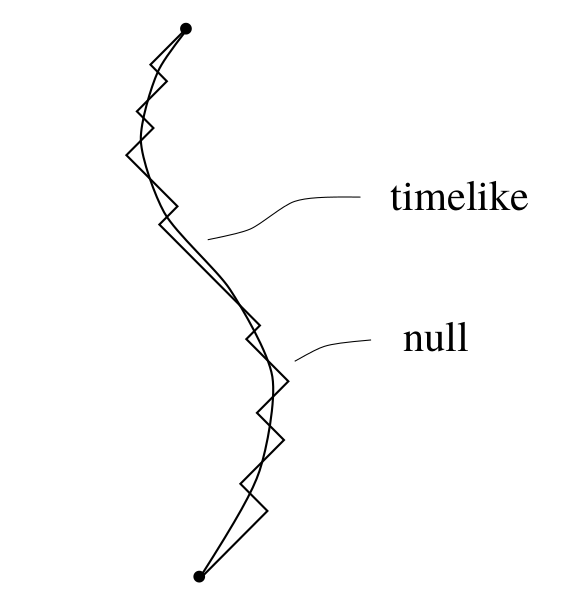
\includegraphics[width=0.7\linewidth]{gfx/ApproximateTimelikeByNullGeodesic}
	\caption{}
	\label{fig:approximatetimelikebynullgeodesic}
\end{figure}
consider “jagged” null curves which follow the timelike one: \\
\todo{I dont understand this argument, shouldnt it be exactly the other way around. I.e. since it is infinitesimally approximated by zero proper time, shouldnt it be minimum proper time ?}
As we increase the number of sharp corners, the null curve comes closer and closer to the
timelike curve while still having zero path length. Timelike geodesics cannot therefore be
curves of minimum proper time, since they are always infinitesimally close to curves of zero
proper time; in fact they maximize the proper time. (This is how you can remember which
twin in the twin paradox ages more — the one who stays home is basically on a geodesic,
and therefore experiences more proper time.)\\
Of course even this is being a little cavalier;
actually every time we say “maximize” or “minimize” we should add the modifier “locally.”
It is often the case that between two points on a manifold there is more than one geodesic.
For instance, on S 2 we can draw a great circle through any two points, and imagine travelling
between them either the short way or the long way around. One of these is obviously longer
than the other, although both are stationary points of the length functional.















\section{An equivalent consideration of parallel transport, geodesics}
Having set up the machinery of connections as exemplified by \ref{fig:flowmanifoldstructure}, the first thing we will do is discuss parallel
transport. Recall that in flat space it was unnecessary to be very careful about the fact
that vectors were elements of tangent spaces defined at individual points; it is actually very
natural to compare vectors at different points (where by “compare” we mean add, subtract,
take the dot product, etc.). The reason why it is natural is because it makes sense, in flat
space, to “move a vector from one point to another while keeping it constant.” Then once
we get the vector from one point to another we can do the usual operations allowed in a
vector space. The concept of moving a vector along a path, keeping constant all the while, is known
as \emph{parallel transport}. As we shall see, parallel transport is defined whenever we have a connection; the intuitive manipulation of vectors in flat space makes implicit use of the
Christoffel connection on this space. The crucial difference between flat and curved spaces is
that, in a curved space, \emph{the result of parallel transporting a vector from one point to another
	will depend on the path taken between the points}.\\
\\
Without yet assembling the complete
mechanism of parallel transport, we can use our intuition about the two-sphere to see that
this is the case. Start with a vector on the equator, pointing along a line of constant
longitude. Parallel transport it up to the north pole along a line of longitude in the obvious
way. Then take the original vector, parallel transport it along the equator by an angle $θ$, and
then move it up to the north pole as before. It is clear that the vector, parallel transported
along two paths, arrived at the same destination with two different values (rotated by $θ$).
\begin{figure}[h!]
	\centering
	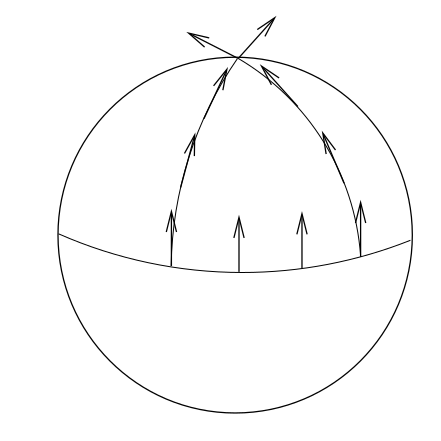
\includegraphics[width=0.7\linewidth]{gfx/ParalleltransportTwosphere}
	\caption{}
	\label{fig:paralleltransporttwosphere}
\end{figure}

It therefore appears as if there is no natural way to uniquely move a vector from one
tangent space to another; we can always parallel transport it, but the result depends on the
path, and there is no natural choice of which path to take. Unlike some of the problems we
have encountered, there is no solution to this one — we simply must learn to live with the
fact that two vectors can only be compared in a natural way if they are elements of the same
tangent space. For example, two particles passing by each other have a well-defined relative
velocity (which cannot be greater than the speed of light). But two particles at different
points on a curved manifold do not have any well-defined notion of relative velocity — the
concept simply makes no sense.\\
In cosmology, for example, the light from distant galaxies
is redshifted with respect to the frequencies we would observe from a nearby stationary
source. Since this phenomenon bears such a close resemblance to the conventional Doppler
effect due to relative motion, it is very tempting to say that the galaxies are “receding away
from us” at a speed defined by their redshift. At a rigorous level this is nonsense, what
Wittgenstein would call a “grammatical mistake” — the galaxies are not receding, since the
notion of their velocity with respect to us is not well-defined. What is actually happening
is that the metric of spacetime between us and the galaxies has changed (the universe has expanded) along the path of the photon from here to there, leading to an increase in the
wavelength of the light. As an example of how you can go wrong, naive application of the
Doppler formula to the redshift of galaxies implies that some of them are receding faster than
light, in apparent contradiction with relativity. The resolution of this apparent paradox is
simply that the very notion of their recession should not be taken literally.
\\
\\
The notion of parallel transport is obviously dependent on the connection, and different
connections lead to different answers. If the connection is metric-compatible, the metric is
always parallel transported with respect to it
\begin{equation}
	\nabla_{\dot{\gamma}} g_{\mu \nu} = \frac{\md x^\sigma}{\md \lambda} \nabla_\sigma g_{\mu \nu} =0.
\end{equation}
It follows that the inner product of two parallel-transported vectors is preserved. This means that parallel transport with respect to a metric-compatible connection preserves
the norm of vectors, the sense of orthogonality.

\subsection{Formal solution to the parallel transport equation}
You can write down an explicit
and general solution to the parallel transport equation, which reads for a tensor
\begin{equation}
	\frac{\md x^\sigma}{\md \lambda} \nabla_\sigma T^{\mu_1 \dots \mu_k}_{\qquad \quad \nu_1 \dots \nu_l}=0
\end{equation}
or for a vector
\begin{equation}
	\frac{\md }{\md \lambda} V^\mu + \Gamma^\mu_{\sigma \rho} \frac{\md x^\sigma}{\md \lambda} V^\rho = 0,
\end{equation}

 although it’s somewhat formal. First
notice that for some path $γ : λ → x^σ (λ)$, solving the parallel transport equation for a vector
$V^\mu$ amounts to finding a matrix $P^μ_ρ (λ, λ_0 )$ which relates the vector at its initial value $V^μ (λ_0 )$
to its value somewhere later down the path:
\begin{equation}
	V^\mu (\lambda) = P^\mu_{\rho}(\lambda, \lambda_0) V^\rho (\lambda_0).
\end{equation}
Of course the matrix $P^μ_ρ (λ, λ_0 )$, known as the \emph{parallel propagator}, depends on the path
$γ$ (although it’s hard to find a notation which indicates this without making γ look like an
index). If we define
\begin{equation}
	A^\mu_\rho (\lambda) = -  \Gamma^\mu_{\rho \sigma} \frac{\md x^\sigma}{\md \lambda},
\end{equation}
where the quantities on the RHS are evaluated at $x^\nu(\lambda)$, then the parallel transport
equation becomes
\begin{equation}
	\frac{\md}{\md \lambda} V^\mu (\lambda) = A^\mu_\rho V^\rho.
\end{equation}
Since the parallel propagator must work for any vector, substituting it in shows
that $P^μ_ρ (λ, λ_0 )$ also obeys this equation:
\begin{equation}
	\frac{\md}{\md \lambda} P^\mu_\rho (\lambda, \lambda_0)= A^\mu_\sigma(\lambda) P^\sigma_\rho(\lambda,\lambda_0).
\end{equation}
To solve this equation, first integrate both sides:
\begin{equation}
P^\mu_\rho (\lambda,\lambda_0) = \delta^\mu_\nu + \int_{\lambda_0}^{\lambda} A^\mu_\sigma (\eta) P^\sigma_\rho(\eta, \lambda_0) \md \eta.
\end{equation}
The Kronecker delta, it is easy to see, provides the correct normalization for $λ = λ_0$ .
We can solve this by iteration, taking the right hand side and plugging it into itself
repeatedly, giving
\begin{equation}
	P^\mu_\rho(\lambda,\lambda_0) = \delta^\mu_\rho + \int_{\lambda_0}^{\lambda} A^\mu_\rho (\eta) \md \eta + \int_{\lambda_0}^\lambda  \int_{\lambda_0}^\eta A^\mu_\sigma(\eta) A^\sigma_\rho (\eta^\prime) \md \eta^\prime \md \eta + \dots 
\end{equation}
The $n$th term in this series is an integral over an $n$-dimensional right triangle, or n-simplex.


\begin{figure}[h!]
	\centering
	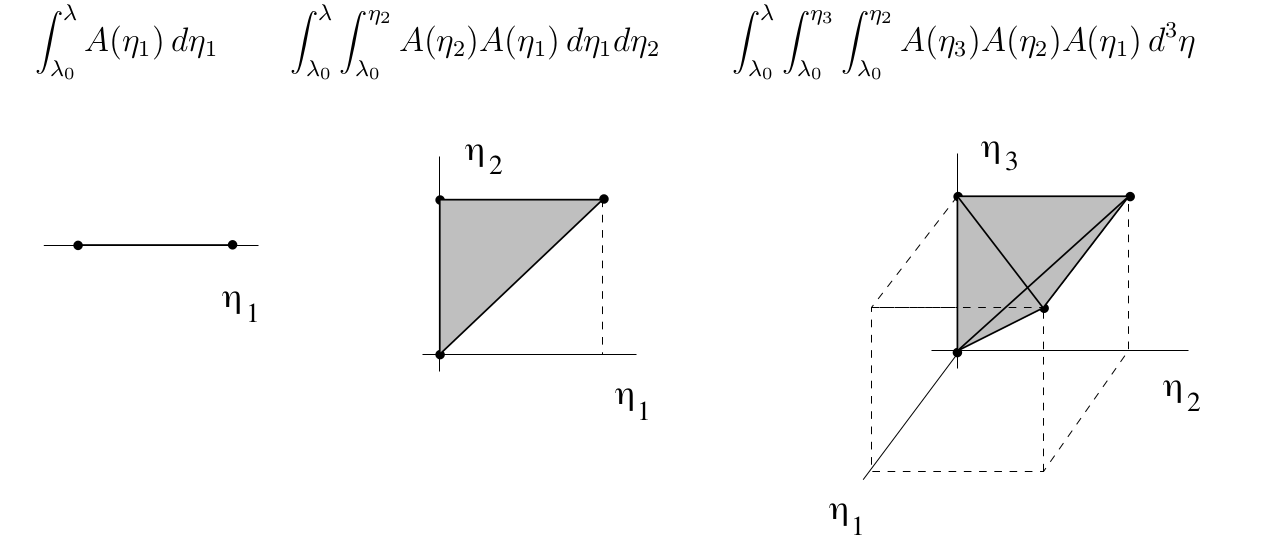
\includegraphics[width=0.7\linewidth]{gfx/SolutionGeodesicEquation}
	\caption{}
	\label{fig:solutiongeodesicequation}
\end{figure}

It would simplify things if we could consider such an integral to be over an $n$-cube
instead of an $n$-simplex; is there some way to do this? There are $n!$ such simplices in each
cube, so we would have to multiply by $1/n!$ to compensate for this extra volume. But we
also want to get the integrand right; using matrix notation, the integrand at $n$th order
is $A(η_n )A(η_{n−1} ) · · · A(η_1 )$, but with the special property that $η_n ≥ η_{n−1} ≥ · · · ≥ η_1$ . We
therefore define the \emph{path-ordering symbol} $\mathcal{P}$ to ensure that this condition holds. In
other words, the expression
\begin{equation}
	\mathcal{P}\left[A(\eta_n) \dots A(\eta_1)\right]
\end{equation}
Stands for the product of the $n$ matrices $A(η_i )$, ordered in such a way that the largest value
of $η_i$ is on the left, and each subsequent value of $η_i$ is less than or equal to the previous one.
We then can express the $n$th-order term in the solution as
\begin{equation}
	\int_{\lambda_0}^\lambda \int_{\lambda_0}^{\eta_n} \dots \int_{\lambda_0}^{\eta_2} A(\eta_n) \dots A(\eta_1) \md^n \eta = \frac{1}{n!}\int_{\lambda_0}^\lambda \int_{\lambda_0}^\lambda \dots \int_{\lambda_0}^\lambda \mathcal{P}\left[A(\eta_n) \dots A(\eta_1)\right] \md^n \eta.
\end{equation}
This yields the solution to the parallel propagator as
\begin{equation}
	P(\lambda,\lambda_0) = \mathcal{I} + \sum_{i=n}^{\infty} \frac{1}{n!} \int_{\lambda_0}^\lambda  \mathcal{P}\left[A(\eta_n) \dots A(\eta_1)\right] \md^n \eta = \mathcal{P} \exp\left(\int_{\lambda_0}^\lambda A(\eta) \md \eta\right).
\end{equation}
Or more explicitly
\begin{equation}
	P^\mu\nu (\lambda, \lambda_0) = \mathcal{P} \exp \left(-\int_{\lambda_0}^\lambda \Gamma^\mu_{\sigma \nu} \frac{\md x^\sigma}{\md \eta}  \md \eta\right).
\end{equation}
The same kind of expression appears in quantum field theory as “Dyson’s Formula,” where it arises because the
Schrödinger equation for the time-evolution operator has the same form as this.\\
\\
As an aside, an especially interesting example of the parallel propagator occurs when the
path is a loop, starting and ending at the same point. Then if the connection is metric-
compatible, the resulting matrix will just be a Lorentz transformation on the tangent space
at the point. This transformation is known as the “holonomy” of the loop. If you know
the holonomy of every possible loop, that turns out to be equivalent to knowing the metric.




\section{Curvature}

The invariant quantities which characterize the geometry in a way which is independent of particular choice of coordinates are curvatures. The curvatures are precisely a measure of the local mismatch between the surface and the tangent plane. Since the tangent space is flat, the derivatives of the components contain no terms due to the curving of the coordinates, and the gradients of vectors w.r.t. flat coordinates are tensors.\\
\\
To compute the covariant derivative of a tensor having many indices the rules is that each index brings an added term involving $\Gamma$ and the tensor itself. Indices can be up or down only in one way and it is only the identification $+$ with up, $-$ with down that needs to be memorized
\\
The fact that the curvature tensor appears as  connecting the second covariant derivatives 
\begin{equation}
A^\mu_{; \sigma \tau} - A^\mu_{;\tau \sigma} = \bar{R}^\mu_{\rho \sigma \tau} A^\rho
\end{equation}
serves as a clue that enables us to give another useful geometrical picture of curvature. The noncommuting property of the second derivatives represents a limit of differences in the vector as we move first a displacement along axis $\sigma$ and then along $\tau$, or first along $\tau$  and the along $\sigma$. If the coordinates are flat, for a constant vector there is no difference. If we have curved space as we take these displacements in different orders, we find different resulting vectors. The curvature $K$ of a surface is defined in terms of the angle through which a vector is turned as we take it around an infinitesimal closed path. The generalized definition of curvature of a many-dimension surface will be given i.t.o. the change in a vector as it is carried about a closed path, keeping it parallel to itself. Since the orientation of a path lying on a definite plane depends on two coordinate axes, we see that the curvature will have the general character of a fourth rank tensor.

\subsection{Torsion and metric connection}
\begin{mybox}{Torsion}
	The torsion $T$ maps two vector field $x$ and $y$ into another vector field 
	\begin{equation}
		T:TM \times TM \rightarrow TM, (x,y) \mapsto T(x,y) = \nabla_x y - \nabla_y x - [x,y],
	\end{equation}
	where the commutator of two vector fields is defined as $[X,Y]^\mu= X^\lambda \partial_\lambda Y^\mu - Y^\lambda \partial_\lambda X^\mu$.
	In components
	\begin{equation}
		T^i_{jk} = \Gamma^i_{jk} - \Gamma^i_{kj}.
	\end{equation}
	The torsion vanishes if and only if the connection is symmetric, i.e. if the Christoffel's are symmetric. The torsion
	quantifies whether parallelograms spanned by two vectors close
\end{mybox}
On a manifold $(M,g)$, a symmetric connection can always be uniquely defined by requiring that $\nabla g=0, \nabla_{\sigma} g_{\mu \nu} =0, \nabla_{\sigma} g^{\mu \nu}=0$. This is the \emph{Levi-Civita, or Riemannian} connection, whose Christoffel symbols are
\begin{equation}
	\Gamma^i_{jk} = \half g^{ia} \left(\partial_j g_{ak} + \partial_k g_{j a}\ - \partial_a g_{jk} \right).
\end{equation}
From now on, we shall assume that we are working with a Levi-Civita connectin whose torsion vanishes.



\subsection{How to get from the connection coefficients to the connection-the metric connection}


To define a covariant derivative, then, we need to put a “connection” on our manifold,
which is specified in some coordinate system by a set of coefficients $Γ^\lambda_{\mu \nu}$ ($n^3 = 64$ independent
components in $n = 4$ dimensions) which transform according to \ref{eq:christoffelTrafo}. (The name “connection” comes from the fact that it is used to transport vectors from one tangent space to
another.) There are evidently a large number of connections we could
define on any manifold, and each of them implies a distinct notion of covariant differentiation. In general relativity this freedom is not a big concern, because it turns out that every
metric defines a unique connection, which is the one used in GR. Let’s see how that works.\\
\\
The first thing to notice is that the difference of two connections is a $(1, 2)$ tensor. If
we have two sets of connection coefficients,$ Γ^{\lambda}_{μν}$ and $\hat{\Gamma}^\lambda_{\mu \nu}$, their difference $S^{\quad \lambda}_{\mu \nu} = \Gamma^\lambda_{\mu \nu} - \hat{\Gamma}^\lambda_{\mu \nu}$ (notice index placement, here it matters since it is a tensor) transforms as
\begin{equation}
S^{\quad \lambda^\prime}_{\mu^\prime \nu^\prime} =..= \frac{\partial x^\mu}{\partial x^{\mu^\prime}} \frac{\partial x^\nu}{\partial x^{\nu^\prime}} \frac{\partial x^{\lambda^\prime}}{\partial x^\lambda} S^{\quad \lambda}_{\mu \nu}
\end{equation}
This is just the tensor transformation law, so $S^\lambda_{\mu \nu}$ is indeed a tensor. This implies that any
set of connections can be expressed as some fiducial connection plus a tensorial correction.
Next notice that, given a connection specified by $Γ^λ_{μν}$ , we can immediately form another
connection simply by permuting the lower indices. That is, the set of coefficients $Γ^λ_{νμ}$ will
also transform according to \ref{eq:christoffelTrafo} (since the partial derivatives appearing in the last term
can be commuted), so they determine a distinct connection. There is thus a tensor we can
associate with any given connection, known as the \emph{torsion tensor}, defined by
\begin{equation}
	T^{\quad \lambda}_{\mu \nu} = \Gamma^\lambda_{\mu \nu} - \Gamma^\lambda_{\nu \mu} = 2 \Gamma^\lambda_{[\mu nu]}.
\end{equation}
It is clear that the torsion is antisymmetric its lower indices, and a connection which is
symmetric in its lower indices is known as “torsion-free.”\\
We can now define a unique connection on a manifold with a metric $g_{μν}$ by introducing
two additional properties:
\begin{enumerate}
\item  torsion-free: $Γ^λ_{μν} = Γ^λ_{ (μν)}$ .
\item Metric compatibility: $\nabla_\rho g_{\mu \nu} =0.$
\end{enumerate}
A connection is \emph{metric compatible} if the covariant derivative of the metric with respect to
that connection is everywhere zero. This implies a couple of nice properties. First, it’s easy
to show that the inverse metric also has zero covariant derivative,
\begin{equation}
	\nabla_\rho g^{\mu \nu} = 0.
\end{equation}
Second, a metric-compatible covariant derivative commutes with raising and lowering of
indices.\\
Our claim is therefore that there is exactly one torsion-free connection on a given manifold
which is compatible with some given metric on that manifold. We do not want to make these
two requirements part of the definition of a covariant derivative; they simply single out one
of the many possible ones. We can demonstrate both existence and uniqueness by deriving a manifestly unique
expression for the connection coefficients in terms of the metric. To accomplish this, we
expand out the equation of metric compatibility for three different permutations of the
indices:
\begin{equation}
	\nabla_\rho g_{\mu \nu} = \partial_\rho - \Gamma^\lambda_{\rho \mu} g_{\lambda \nu} - \Gamma^\lambda_{\rho \nu} g_{\lambda \mu}, \quad \nabla_\nu g_{\rho \mu} = ....
\end{equation}
Manipulating these equations yields the unique form of the Christoffel symbols for the metric connection
\begin{equation}
\label{eq:Christoffels}
	\Gamma^\sigma_{\mu \nu} = \frac{1}{2} g^{\sigma \rho} \left[\partial_{\mu} g_{\nu \rho} + \partial_\nu g_{\rho \mu} - \partial_\rho g_{\mu \nu} \right].
\end{equation}
This is one of the most important formulas in this subject; commit it to memory. Of course,
we have only proved that if a metric-compatible and torsion-free connection exists, it must
be of the form \ref{eq:Christoffels}; you can check for yourself (for those of you without enough tedious
computation in your lives) that the right hand side of \ref{eq:Christoffels} transforms like a connection.
This connection we have derived from the metric is the one on which conventional general
relativity is based (although we will keep an open mind for a while longer). It is known
by different names: sometimes the \emph{Christoffel connection}, sometimes the \emph{Levi-Civita
connection}, sometimes the \emph{Riemannian connection}. The associated
connection coefficients are sometimes called Christoffel symbols. The study of manifolds with
metrics and their associated connections is called “Riemannian geometry.”\\
\\
Let’s emphasize again that the connection does \emph{not have to be} constructed
from the metric. In ordinary flat space there is an implicit connection we use all the time
— the Christoffel connection constructed from the flat metric. But we could, if we chose,
use a different connection, while keeping the metric flat. Also notice that the coefficients
of the Christoffel connection in flat space will vanish in Cartesian coordinates, but not in
curvilinear coordinate systems. The existence of nonvanishing connection coefficients in curvilinear coordinate systems is
the ultimate cause of the formulas for the divergence and so on that you find in books on
electricity and magnetism.

\subsection{Conceptional flow of how to add structure on our mathematical constructs}
Before moving on, let’s review the process by which we have been adding structures to
our mathematical constructs. We started with the basic notion of a set, which you were
presumed to know (informally, if not rigorously). We introduced the concept of open subsets
of our set; this is equivalent to introducing a topology, and promoted the set to a topological
space. Then by demanding that each open set look like a region of $\mR^n$ (with $n$ the same for
each set) and that the coordinate charts be smoothly sewn together, the topological space
became a manifold. A manifold is simultaneously a very flexible and powerful structure,
and comes equipped naturally with a tangent bundle, tensor bundles of various ranks, the
ability to take exterior derivatives, and so forth. We then proceeded to put a metric on
the manifold, resulting in a manifold with metric (or sometimes “Riemannian manifold”).
Independently of the metric we found we could introduce a connection, allowing us to take
covariant derivatives. Once we have a metric, however, there is automatically a unique
torsion-free metric-compatible connection. (In principle there is nothing to stop us from
introducing more than one connection, or more than one metric, on any given manifold.)
\begin{figure}[h!]
	\centering
	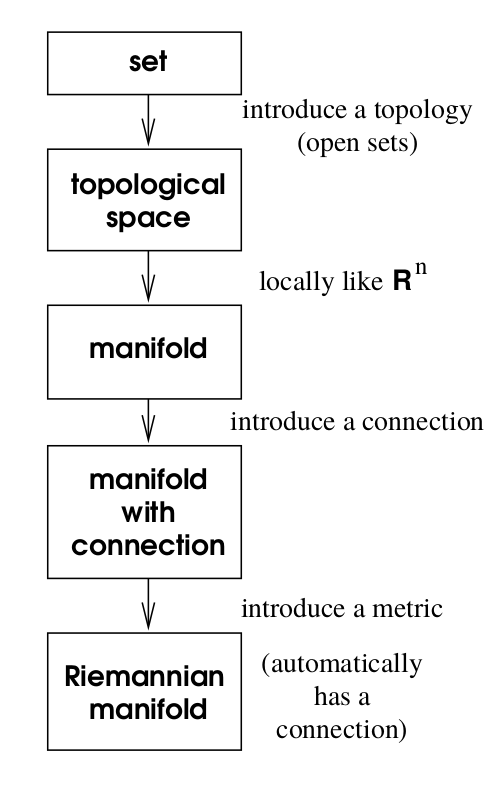
\includegraphics[width=0.7\linewidth]{gfx/FlowManifoldStructure}
	\caption{}
	\label{fig:flowmanifoldstructure}
\end{figure}

\subsection{The curvature}
The idea behind this measure of curvature, the Riemann tensor which is derived from the connection, is that we
know what we mean by “flatness” of a connection — the conventional (and usually implicit)
Christoffel connection associated with a Euclidean or Minkowskian metric has a number of
properties which can be thought of as different manifestations of flatness. These include the
fact that parallel transport around a closed loop leaves a vector unchanged, that covariant
derivatives of tensors commute, and that initially parallel geodesics remain parallel. It would be more useful to have a local description of the curvature at each point, which is what the Riemann tensor is supposed to provide. One conventional way to introduce the
Riemann tensor, therefore, is to consider parallel transport around an infinitesimal loop.\\
We want to construct a tensor out of the metric and its derivatives. If we use only $g\munu$ and its first derivatives, then no new tensor can be constructed, for at any point we can find a coordinate system (RNC) in which the first deriavtives of the metric tensor vanish, so in this coordinate system the desired tensor must be equal to one of those that can be constructed out of the metric tensor \emph{alone}, and since this is an equality between tensors it must be true in all coordinate systems. Hence our search for this tensor is motivated by the Principle of General Covariance.
\begin{mybox}{Curvature and Curvature tensor}
	The curvature $\bar{R}$ maps three vector field $x,y$ and $v$ into a vector field,
	\begin{align}
		\bar{R}:TM\times TM \times TM &\rightarrow TM,\\
		 (x,y,z) \mapsto \bar{R}(x,y) v &= \nabla_x(\nabla_y v) - \nabla_y(\nabla_x v) \nabla_{[x,y]} v.
	\end{align} 
Note that the two vectors $x$ and $y$ appearing here correspond
to the two antisymmetric indices in the component form of the Riemann tensor. The last
term, involving the commutator $[x, y ]$, vanishes when $x$ and $y$ are taken to be
the coordinate basis vector fields (since $[∂_μ , ∂_ν ] = 0$), which is why this term did not arise
when we take the commutator of two covariant derivatives as performed below.\\
Since the covariant derivatives $\nabla_x$ and $\nabla_y$ represent the infinitesimal parallel transports along the integral curves of the vector fields $x$ and $y$, the curvature $\bar{R}$ directly quantifies the change of the vector $v$ when it is parallel-transported around an infinitesimal, closed loop.
\\
The \emph{curvature or Riemann tensor} $\bar{R} \in \mathcal{T}^1_3$ is given by 
\begin{equation}
\bar{R}:T^*M\times TM \times TM \times TM \rightarrow \mR, (w,x,y,z) \mapsto w[\bar{R}(x,y)z].
\end{equation}
Its components are 
\begin{align}
\bar{R}^i_{\; j k l} &= \md x^i [\bar{R}(\partial_k, \partial_l) \partial_j] \\
							&= \partial_k \Gamma^i_{jl} - \partial_l \Gamma^i_{jk} + \Gamma^a_{jl} \Gamma^i_{ak} - \Gamma^a_{jk} \Gamma^i_{al}.
\end{align}
The Riemann tensor is antisymmetric, i.e. $i=j => \bar{R}=0$ and obeys $3$ further symmetries 
\begin{align}
	\bar{R}_{ijkl} &= -\bar{R}_{jikl} =\bar{R}_{jilk} \\
	\bar{R}_{ijkl} &= \bar{R}_{klij}
\end{align}
such that it only has $21$ independent components.\\
All of the components of $\bar{R}^{\sigma}_{\mu \alpha \beta}$ vanish if and only if the space is flat. Operationally, "flat" means that there exists a global coordinate system in which the metric components are everywhere constant.
\end{mybox}
One can equivalently find the form of the Riemann tensor by considering a related operation, the commutator of two covariant derivatives. The relationship between this and parallel transport around a loop should be evident;
the covariant derivative of a tensor in a certain direction measures how much the tensor
changes relative to what it would have been if it had been parallel transported (since the
covariant derivative of a tensor in a direction along which it is parallel transported is zero).
The commutator of two covariant derivatives, then, measures the difference between parallel
transporting the tensor first one way and then the other, versus the opposite ordering.
\begin{equation}
	[\nabla_\mu, \nabla_\nu] V^\rho = ..= \underbrace{\left(\partial_\mu \Gamma^\rho_{\nu \sigma} - \partial_\nu \Gamma^\rho_{\mu \sigma} + \Gamma^\rho_{\mu \lambda}\Gamma^\lambda_{\nu \sigma} -\Gamma^\rho_{\nu \lambda}\Gamma^\lambda_{\mu \sigma} \right)}_{\bar{R}^\rho_{\sigma \mu \nu}} V^\sigma - \underbrace{2 \Gamma^\lambda_{[\mu \nu]}}_{T^{\,\, \lambda}_{\mu\nu}} \nabla_\lambda V^\rho.
\end{equation}
Note:\\
The Riemann tensor measures that part of
the commutator of covariant derivatives which is proportional to the vector field, while
the torsion tensor measures the part which is proportional to the covariant derivative
of the vector field; the second derivative doesn’t enter at all.\\
\\
Having defined the curvature tensor as something which characterizes the connection, let
us now admit that in GR we are most concerned with the Christoffel connection. In this
case the connection is derived from the metric, and the associated curvature may be thought
of as that of the metric itself. This identification allows us to finally make sense of our
informal notion that spaces for which the metric looks Euclidean or Minkowskian are flat.
In fact it works both ways: if the components of the metric are constant in some coordinate
system, the Riemann tensor will vanish, while if the Riemann tensor vanishes we can always
construct a coordinate system in which the metric components are constant\\
\\
\subsection{Independent components of the Riemann tensor and intuition for curvature}
Given these relationships between the different components of the Riemann tensor, how
many independent quantities remain? Let’s begin with the facts that $\bar{R}_{ρσμν}$ is antisymmetric
in the first two indices, antisymmetric in the last two indices, and symmetric under interchange of these two pairs. This means that we can think of it as a symmetric matrix $\bar{R}_{[ρσ][μν]}$ ,
where the pairs $ρσ$ and $μν$ are thought of as individual indices. An $ m × m$ symmetric matrix has $m(m + 1)/2$ independent components, while an $n × n$ antisymmetric matrix has
$n(n − 1)/2$ independent components. We therefore have
\begin{equation}
	\half \left[\half n(n-1)\right]\left[\half n(n-1) +1\right] = \frac{1}{8} \left(n^4-2n^3+3n^2- 2n\right)
\end{equation}
independent components. The first Bianchi identity implies together with the antisymmetry of the Riemann tensor that $\bar{R}_{[\rho\sigma\mu\nu]}=0$.
Now a totally antisymmetric $4$-index tensor has $n(n−1)(n−2)(n−3)/4!$ terms, and therefore we are left with
\begin{equation}
\label{eq:dofRiemann}
	 \frac{1}{8} \left(n^4-2n^3+3n^2- 2n\right)-n(n−1)(n−2)(n−3)/4! = \frac{1}{12} n^2 (n^2-1)
\end{equation}
independent components, i.e. $20$ for $n=4$ spacetime dimensions.\\
\\\marginpar{ A curvature radius is only appropriate for "extrinsic" curvature – the curvature of a line/submanifold embedded into a higher-dimensional space. The Riemann tensor measures all the components of the intrinsic curvature so they're not exactly the same. }
After this large amount of formalism, it might be time to step back and think about what
curvature means for some simple examples. First notice that, according to \ref{eq:dofRiemann}, in $1, 2, 3$
and $4$ dimensions there are $0, 1, 6$ and $20$ components of the curvature tensor, respectively.
(Everything we say about the curvature in these examples refers to the curvature associated
with the Christoffel connection, and therefore the metric.) This means that one-dimensional
manifolds (such as $S^1$, i.e. a circle ) are never curved; the intuition you have that tells you that a circle is
curved comes from thinking of it embedded in a certain flat two-dimensional plane. (There is
something called “extrinsic curvature,” which characterizes the way something is embedded
in a higher dimensional space. Our notion of curvature is “intrinsic,” and has nothing to do
with such embeddings.)\\
The distinction between intrinsic and extrinsic curvature is also important in two dimensions, where the curvature has one independent component. (In fact, all of the information about the curvature is contained in the single component of the Ricci scalar.)\\
Consider a
cylinder, $\mR × S^1$ . Although this looks curved from our point of view, it should be clear
that we can put a metric on the cylinder whose components are constant in an appropriate
coordinate system — simply unroll it and use the induced metric from the plane. In this
metric, the cylinder is flat. (There is also nothing to stop us from introducing a different
metric in which the cylinder is not flat, but the point we are trying to emphasize is that it
can be made flat in some metric.)
\begin{figure}[h!]
	\centering
	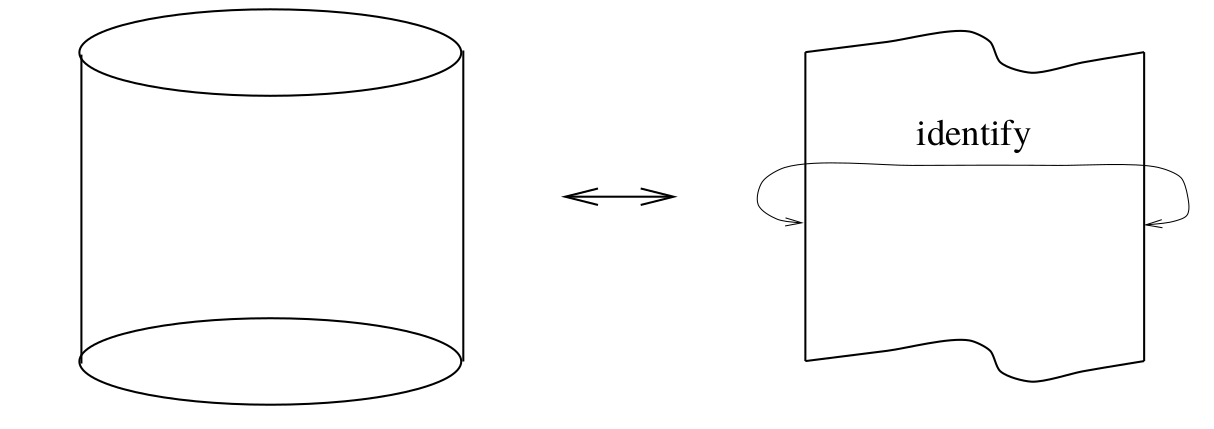
\includegraphics[width=0.7\linewidth]{gfx/CurvatureCylinder}
	\caption{\itshape I.e. cylinder is not curved since it can be glued together by flat spaces.}
	\label{fig:curvaturecylinder}
\end{figure}
Positively curved spaces have a positively curved Ricci scalar, whereas flat spaces have a vanishing one etc.


\subsubsection{Uniqueness by General Covariance ? Weinberg}
The existence of the tensor $\bar{R}^\rho_{\mu \lambda \nu}$ raises the question of whether or not the Principle of Equivalence or the Principle of General Covariance uniquely determines the effects of gravitation on arbitrary physical systems. For instance, let us ask whether the correct e.o.m. for a freely falling particle of spin $S_\mu$ might be of the form
\begin{equation}
	0 = \frac{\md^2 x^\lambda}{\md \tau^2} + \Gamma^\lambda_{\mu \nu} \frac{\md x^\mu}{\md \tau} \frac{\md x^\nu}{\md \tau} + f R^\lambda_{\mu \nu \kappa} \frac{\md x^\mu}{\md \tau} \frac{\md x^\nu}{\md \tau} S^\kappa
\end{equation}
(with $f$ and unknown scalar) instead of the familiar geodesic equation \ref{eq:geodesicequation}. Both equations are generally covariant, and both reduce in the absence of gravitation to be correct special-relativistic equation $\md U^\alpha /\md \tau =0$. How then can we tell whether one or the other is correct ?\\
The answer is one of \emph{scale}. Suppose that our particle has a characteristic linear dimension $d$, and that the gravitational field has a characteristic space-time dimension $D$. The Riemann tensor has one more derivative of the metric than the affine connection coefficients, so the ratio of the third term in the first equation to the second term is proportional to $1/D$; dimensional considerations then require that this ratio be roughly of order $d/D$. Thus, barring special circumstances that might make one term or the other anomalously large or small, we can regard the last term in the first equation as being negligible if our particle is very much smaller than the characteristic dimensions of the gravitational field, and the geodesic equation is the correct e.o.m. Of course, if our particle is not much smaller than the gravitational field scale (as in the case of the moon moving in the gravitational field of the earth), then the Principle of Equivalence or the Principle of General Covariance must be applied to the infinitesimal elements of which the particle is composed, although both equations might give a fair phenomenological representation of the motion of the whole particle.\\
\\
Note further that one can prove that the Riemann tensor is the \emph{only} tensor that can be constructed from the metric tensor and its first and second derivatives, and is linear in the second derivatives.






\subsection{The Ricci tensor}
The symmetry in the first and last index pair of the Riemann tensor shows that the Ricci tensor is symmetric. Furthermore, the antisymmetry of the Riemann tensor in the first and last index pair tells us that the Ricci tensor is essentially the only second-rank tensor that can be formed from the Riemann tensor, since
multiplying the antisymmetry condition of the Riemann tensor with $g^{\lambda \nu}$, $g^{\lambda \mu}$, and $g^{\nu \kappa}$ gives
\begin{equation}
	R_{\mu \kappa} = -g^{\lambda \nu} \bar{R}_{\mu \lambda \nu \kappa} = - g^{\lambda \nu} \bar{R}_{\lambda \mu \kappa \nu} = + g^{\lambda \nu} \bar{R}_{\mu\lambda \kappa \nu}
\end{equation}
and 
\begin{equation}
	g^{\lambda \mu} \bar{R}_{\lambda \mu \nu \kappa} = g^{\nu \kappa} \bar{R}_{\lambda \mu \nu \kappa}=0.
\end{equation}
From the antisymmetry property of the Riemann tensor we also see that there is essentially only one way of contracting the Riemann tensor to construct a scalar:
\begin{equation}
	\mathcal{R}=g^{\lambda \nu} g^{\mu \kappa} \bar{R}_{\lambda \mu \nu \kappa} = - g^{\lambda \nu} g^{\mu \kappa} \bar{R}_{\mu \lambda \nu \kappa}, \; 0 = g^{\lambda \mu} g^{\nu \kappa} \bar{R}_{\lambda \mu \nu \kappa}.
\end{equation}
\begin{mybox}{Ricci tensor}
	The symmetric \emph{Ricci tensor} $R$ is the contraction $C^1_3 \bar{R}$ of the curvature tensor $\bar{R}$. Its components are 
	\begin{equation}
		R_{jl} = \bar{R}^i_{jil} = g^{i m} \bar{R}_{mjil}=\partial_i \Gamma^i_{lj} - \partial_l \Gamma^i_{ij} + \Gamma^m_{lj} \Gamma^i_{im} - \Gamma^m_{ij} \Gamma^i_{lm}.
	\end{equation}
	For a symmetric connection with a vanishing torsion, the \emph{Bianchi identity} 
	\begin{equation}
	\nabla_{[\lambda} \bar{R}_{\rho \sigma] \mu \nu} =0
	\end{equation}
	reduces to 
	\begin{align}
	\bar{R}_{\rho \sigma \mu \nu} + \bar{R}_{\rho \mu \nu \sigma}+\bar{R}_{\rho \nu \sigma \mu} & = 0,\\
	 				\nabla_\lambda \bar{R}_{\rho \sigma \mu \nu}+\nabla_\rho \bar{R}_{\sigma \lambda \mu \nu}+\nabla_\sigma\bar{R}_{\lambda \rho \mu \nu} &=0.
	\end{align}
	The contracted Ricci tensor yields the \emph{Ricci scalar}
	\begin{equation}
	 \mathcal{R} = R^i_i = tr(R).
	\end{equation}
	The \emph{contracted Bianchi identitiy} then reads
	\begin{equation}
		\left[R^i_j -\frac{\mathcal{R}}{2} \delta^i_j\right]_{;i} = 0.
	\end{equation}
	One then has the relation
	\begin{align}
		\bar{R}_{\lambda \mu \nu \kappa} &= g_{\lambda \nu} R_{\mu \kappa} - g_{\lambda \kappa} R_{\mu \nu} - g\munu R_{\lambda \kappa} + g_{\mu \kappa} R_{\lambda \nu} \nonumber \\
		&- \half \left[g_{\lambda\nu} g_{\mu \kappa} - g_{\lambda\kappa} g\munu\right] \mathcal{R}.
	\end{align}
\end{mybox}
\subsection{The Einstein tensor}
The symmetric \emph{Einstein tensor} is given by
\begin{equation}
G_{ij} = R_{ij}  -\frac{\mathcal{R}}{2} g_{ij},
\end{equation}
which has vanishing divergence by the twice contracted Bianchi identity $\nabla^{\mu} G_{\mu \nu} = 0$ $\leftrightarrow$ $G^i_{jji} =0$.
The Einstein tensor is symmetric due to the symmetry of the Ricci tensor and the
metric.


















\section{The Lie derivative}
Another important tensorial derivative is the \emph{Lie derivative}, which is independent of the metric. Whereas the covariant derivative required an affine connection to allow comparison between vectors at different points, the Lie derivative uses a congruence from a vector field to achieve the same purpose. In GR, a congruence is the set of integral curves of a vector field in a $4-d$ manifold.\\
The idea of Lie dragging a function along a congruence leads to the definition of the Lie derivative, wehre the dragged function is compared with the value of the original function at a given point. It is defined as 
\begin{equation}
\mathcal{L}_x :\mathcal{T}^r_s \rightarrow \mathcal{T}^r_s,
\end{equation}
where $x$ is the vector field along whose congruence the Lie derivative is taken.\\
The Lie derivative of a scalar is just the directional derivative.\\
\\
\subsection{Pull-back and Push-forward}
A differentiable curve $\gamma_t(p)$ defined at every point $p \in M$ defines a diffeomorphic map $\phi_t:M\rightarrow M$. If $\dot{\gamma}_t=v$ for a vector field $v \in TM$, $\phi_t$ is called the \emph{flow} of $v$ .If a tangent vector defined by 
\begin{equation}
	(\dot{\gamma}(t))(f) = \frac{\md }{\md t} (f \circ \gamma) (t)
\end{equation}
suffices $\dot{\gamma}=v$, then $\gamma$ is called an \emph{integral curve} of $v$. Equivalently, given a coordinate system $x^μ$ on
M , the components of $\dot{\gamma}$ in that coordinate system must satisfy
\begin{equation}
	\dot{\gamma}^\mu = \frac{\md}{\md t} x^\mu (\gamma(t)),
\end{equation}
where $t$ parametrizes the curve $\gamma$, could also choose $\lambda$ etc.\\

If this is true for all curves $\gamma$ obtained from $\gamma_t$ by specifying $\gamma(0)$, the result is called flow of v.
\begin{figure}[h!]
	\centering
	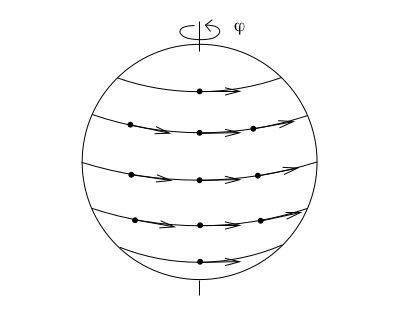
\includegraphics[width=0.7\linewidth]{gfx/IntegralCurvesTwoSphere}
	\caption{\itshape E.g. integral curves on the two-sphere, defining the rotations by a given angle. The tangent vectors infinitesimmaly generate the rotation. Compare treatment in \ref{subsubsec:tangentvectors}.}
	\label{fig:integralcurvestwosphere}
\end{figure}
Our diffeomorphisms $φ_t$ represent “flow down the integral
curves,” and the associated vector field is referred to as the generator of the diffeomorphism.
(Integral curves are used all the time in elementary physics, just not given the name. The
“lines of magnetic flux” traced out by iron filings in the presence of a magnet are simply the
integral curves of the magnetic field vector $\vec{B}$.)\\
\\
When $\dot{\gamma}$ is smooth and everywhere non-zero, the set of integral curves form a
\emph{congruence}: every point $p \in M$ lies on a unique integral curve. Given any congruence
there is an associated one-parameter family of diffeomorphisms from $M$ onto itself,
defined as follows: for each $s \in \mR$, define $h_s : M → M $, where $h_s (p)$ is the point
parameter distance $s$ from $p$ along $\dot{\gamma}$, i.e. if $p = γ(λ_0 )$ then $h_s (p) = γ(λ_0 + s)$. These
transformations form an abelian group: the composition law is $h_s ◦ h_t = h_s+t$ , the
identity is $h_0$ and the inverse is $(h_s )_{ −1} = h_{ −s}$ .




\begin{mybox}{Pull-back}
	Let now $M$ and $N$ be two manifolds and $\phi: M\rightarrow N$ a map from $M$ onto $N$. A function $f$ defined at a point $q\in N$ can be defined at a point $p\in M$ with $q=\phi(p)$ by 
	\begin{equation}
		\phi^* f : M\rightarrow \mR ,\; (\phi^* f)(p) := (f \circ \phi)(p) = f[\phi(p)].
	\end{equation}
	The map $\phi^*$ "pulls" function $f$ on $N$ "back" to $M$.
\end{mybox}
\begin{mybox}{push-forward}
	Similarly for vectors: $\phi_*:T_pM \rightarrow T_q N$, $v$ $\mapsto \phi_* v=v \circ \phi^*$ such that $(\phi_* v)(f) = v(\phi^* f) = v(f \circ \phi)$, where $q=\phi(p)$.\\
	The map $\phi_*$ "pushes" vectors from the tangent space of $M$ in $p$ to the tangent space of $N$ in $q$.
\end{mybox}
Equivalently extended
\begin{enumerate}
	\item Dual vectors: 
	\begin{equation}
		\phi^*:T^*_q M \rightarrow T^*_p M, \; w \mapsto \phi^* w = w \circ \phi_*,
	\end{equation}
	such that $(\phi^* w)(v) = w(\phi_* v) = w(v \circ \phi^*)$.
	\item Tensors:\\
	 		Pull-back \begin{equation}
	 		 \phi^*: \mathcal{T}^r_s(N) \rightarrow \mathcal{T}^r_s(M),
	 		\end{equation}
	 		push forward
	 		\begin{equation}
	 			\phi_*:\mathcal{T}^r_s(M) \rightarrow \mathcal{T}^r_s(N).
	 		\end{equation}
\end{enumerate}
The important point is that if $\phi^*:M\rightarrow M$ is a diffeomorphism and $T$ is a tensor field $M$, then $\phi^*T$ can be compared to $T$.\marginpar{If $\phi$ is a diffeomorphism $\phi_* = (\phi^*)^{-1}$.}\\
\\
Symmetry transformations:\\
If $\phi^*T=T, \phi^*$ is a symmetry (transformation) of $T$ because $T$ stays the same even though it was "moved" by $\phi^*$.  Although symmetries may be discrete, it is more common to have a one-parameter family
of symmetries $\phi_t$ . If the family is generated by a vector field $V^μ (x)$, then $\phi^*T=T$ is equivalent to
\begin{equation}
	\mL_V T=0.
\end{equation}
If the tensor field is the metric $g$, such a symmetry transformation of $g$ is called an \emph{isometry}. If a one-parameter family of isometries
is generated by a vector field $V^μ (x)$, then $V^μ$ is known as a \emph{Killing vector field}.\\
One implication of a symmetry is that, if $-T$ is symmetric under some one-parameter
family of diffeomorphisms, we can always find a coordinate system in which the components
of $T$ are all independent of one of the coordinates (the integral curve coordinate of the
vector field). The converse is also true; if all of the components are independent of one
of the coordinates, then the partial derivative vector field associated with that coordinate
generates a symmetry of the tensor.
\\
\\
This is a little abstract, and it would be nice to have a more concrete description, go into coordinate tetrad of manifold, i.e. basis on $M$ is $\{\frac{\partial }{\partial x^\mu} \}$ while basis on $N$ is given by $\{\frac{\partial}{\partial y^\alpha}	\}$. Then
\begin{equation}
	(\phi^* V )^α ∂_α f = V^μ ∂_μ (\phi_* f ) =  V^μ ∂_μ (f \circ \phi) = V^\mu \frac{\partial y^\alpha}{\partial x^\mu} \partial_\alpha f.
\end{equation}
This simple formula makes it irresistible to think of the pushforward operation $\phi^∗$ as a matrix
operator, $(\phi^* V )^α = (φ^∗ )^α_μ V^μ$ , with the matrix being given by
\begin{equation}
	(\phi^*)^\alpha_\mu = \frac{\partial y^\alpha}{\partial x^\mu}.
\end{equation}
The behavior of a vector under a pushforward thus bears an unmistakable resemblance to the
vector transformation law under change of coordinates. In fact it is a generalization, since
when $M$ and $N$ are the same manifold the constructions are (as we shall discuss) identical;
but don’t be fooled, since in general $μ$ and $α$ have different allowed values, and there is no
reason for the matrix $∂y^α /∂x_μ$ to be invertible.
Although you can push vectors forward
from $M$ to $N$ (given a map $φ : M → N$), you cannot in general pull them back. 
\\
\\
Since one-forms are dual to vectors, you should not be surprised to hear that one-forms can
be pulled back (but not in general pushed forward).
Once again, there is a simple matrix description of the pullback operator on forms, $(\phi_* ω)_μ =
(φ_∗ )^{\; \; \alpha}_μ ω_α$ , which we can derive using the chain rule. It is given by
\begin{equation}
	(\phi_*)^\alpha_\mu = \frac{\partial y^\alpha}{\partial x^\mu}.
\end{equation}
\\
\\
Fortunately, the matrix representations of the pushforward and pullback extend to
the higher-rank tensors simply by assigning one matrix to each index; thus, for the pullback
of a $(0, l)$ tensor, we have
\begin{equation}
(\phi_∗ T )_{ μ_1 \dots μ_l} = \frac{\partial y^{\alpha_1}}{\partial x^{\mu_1}} \dots \frac{\partial y^{\alpha_l}}{\partial x^{\mu_l}} T_{\alpha_1 \dots \alpha_l},
\end{equation}
while for the pushforward of a $(k, 0)$ tensor we have
\begin{equation}
	(\phi^* S)^{\alpha_1 \dots \alpha_k} = \frac{\partial y^{\alpha_1}}{\partial x^{\mu_1}} \dots \frac{\partial y^{\alpha_k}}{\partial x^{\mu_k}} S^{\mu_1 \dots \mu_k}.
\end{equation}
Note that tensors with both upper and lower indices can generally be neither pushed forward
nor pulled back.\\
\\
One common occurrence of a map between two manifolds is when $M$ is actually a
submanifold of $N$; then there is an obvious map from $M$ to $N$ which just takes an element
of $M$ to the “same” element of $N$. Consider our usual example, the two-sphere embedded in
$\mR^3$ , as the locus of points a unit distance from the origin. If we put coordinates $x^μ = (θ, φ)$
on $M = S^2$ and $y^α = (x, y, z)$ on  $N = \mR^3$ , the map $φ : M → N$ is given by
\begin{equation}
\varphi(\theta, \phi) = ( \sin\theta \cos \phi, \sin\theta \sin \phi, \cos \theta)^T.
\end{equation}
In the past we have considered the metric $ds^2 = dx^2 + dy^2 + dz^2$ on $\mR^3$ , and said that it
induces a metric $dθ^2 + \sin^2 θ dφ^2$ on $S^2$ , just by substituting $\phi(\theta,\phi)$ into this flat metric on $\mR^3$. We didn’t really justify such a statement at the time, but now we can do so. (Of course
it would be easier if we worked in spherical coordinates on $\mR^3$ , but doing it the hard way is
more illustrative.) The matrix of partial derivatives is given by
\begin{equation}
\frac{\partial y^\alpha}{\partial x^\mu} = \begin{pmatrix}
\cos \theta \cos \phi & \cos \theta \sin \phi & -\sin \theta \\
\sin \theta (-\sin\phi) & \sin \theta \cos \phi & 0 
\end{pmatrix}.
\end{equation}
The metric on $S^2$ is obtained by simply pulling back the metric from $\mR^3$ 
\begin{equation}
	(\phi^* g)_{\mu \nu} = \frac{\partial y^\alpha}{\partial x^\mu} \frac{\partial y^\beta}{\partial x^\nu} g_{\alpha \beta} = \begin{pmatrix}
	1 &0 \\ 0 & \sin^2 \theta
	\end{pmatrix}.
\end{equation}
We have been careful to emphasize that a map $φ : M → N$ can be used to push certain
things forward and pull other things back. The reason why it generally doesn’t work both
ways can be traced to the fact that $φ$ might not be invertible.\\
If it is, then it is called a diffeomorphism and we get the general expression for the push-forward
\begin{equation}
	(\phi^* T)^{\alpha_1 \dots \alpha_k}_{\quad \quad \beta_1\dots \beta_l} = \frac{\partial y^{\alpha_1}}{\partial x^{\mu_1}} \dots \frac{\partial y^{\alpha_k}}{\partial x^{\mu_k}} \frac{\partial x^{\nu_1}}{\partial y^{\beta_1}} \dots \frac{\partial x^{\nu_l}}{\partial y^{\beta_l}} T^{\mu_1 \dots \mu_k}_{\quad \quad \nu_1 \dots \nu_l},
\end{equation}
the equation for the push-back is then obtained via $\phi_* = [\phi^{-1}]^*$.

 \subsection{Connection between coordinate transformations and diffeomorphism}
The relationship is that they are two different ways of doing precisely
the same thing. If you like, diffeomorphisms are “active coordinate transformations”, while
traditional coordinate transformations are “passive.” Consider an n-dimensional manifold
$M$ with coordinate functions $x^μ : M → \mR^n$ . To change coordinates we can either simply
introduce new functions $y^μ : M → \mR^n$ (“keep the manifold fixed, change the coordinate
maps”), or we could just as well introduce a diffeomorphism $φ : M → M$, after which the
coordinates would just be the pullbacks $(φ^∗ x)^ μ : M → \mR^n$ (“move the points on the manifold, and then evaluate the coordinates of the new points”).


\subsection{The Lie derivative}
\begin{mybox}{Lie derivative}
	While the covariant derivative determines how vectors and tensors change when moved across a given manifold, the Lie derivative determines how these objects change upon transformations of the manifold itself.\\
	Let now $v$ be a vector field on $M$ and $\gamma_t$ be the flow of $v$. Then, for an arbitrary tensor $T\in \mathcal{T}^r_s$, the expression 
	\begin{equation}
		\mathcal{L}_v T := \lim_{t \rightarrow 0} \frac{\gamma^*_t T-T}{t}
	\end{equation}
	is called \emph{Lie derivative} of the tensor $T$ w.r.t. $v$.\\
	The Lie derivative of a rank-$(0,2)$ tensor $T$ along the vector field $v$ with flow $\phi_t$ has the components
	\begin{equation}
		\left(\mathcal{L}_v T\right)_{ij} =  \lim_{t \rightarrow 0} \left(\frac{\gamma^*_t T-T}{t}\right)_{ij} = v^k \partial_k T_{ij} + \partial_i v^k T_{kj} + \partial_j v^k T_{ik}
	\end{equation}
	where $\phi^*_t T$ is the pull-back of $T$ with $\phi_t$. The Lie derivative of a general tensor field is
	\begin{align*}
		\mL_V T^{ μ_1 \dots μ_k}_{\nu_1 \dots \nu_l} &= V^σ ∂_σ T^{μ_1\dots μ_k}_{ ν_1\dots ν_l} \\
		& −(∂_λ V^{μ_1} )T^{ λμ_2 \dots μ_k}_{ ν_1 ν_2\dots ν_l} − (∂_λ V^{ μ_2} )T^{μ_1 λ\dots μ_k}_{ ν_1 ν_2 \dots ν_l} − · · · \\
		& +(∂_{ν_1} V^λ )T^{ μ_1\dots μ_k}_{ λν_2 \dots ν_l} + (∂_{ν_2}  V^λ )T^{ μ_1 μ_2 \dots μ_k}_{ ν_1 λ\dots ν_l} + · · ·
	\end{align*}
which is manifestly covariant, since one can simply replace $\partial_\mu \leftrightarrow \nabla_\mu$ where $\nabla_\mu$ is any symmetric (torsion-free) covariant derivative (including, of course one derived from a metric).
\end{mybox}
The tensor $T$ on the manifold after the transformation $\gamma_t$ of the manifold is pulled back to the manifold $\gamma^*_t T$ before the transformation, where it can be compared to $T$.\\
\\
The Killing equation can be brought into the useful form
\begin{align}
	\label{eq:liederivMetric}
	\mL_V g_{\mu \nu} &= V^\sigma \nabla_\sigma g_{\mu \nu} + (\nabla_\mu V^\lambda) g_{\lambda \nu} + (\nabla_\nu V^\lambda) g_{\mu \lambda} \\
	&= \nabla_\mu V_\nu + \nabla_\nu V_\mu \\
	&= 2 \nabla_{(\nu} V_{\mu)}.
\end{align}
The Lie derivative has the following properties:
\begin{enumerate}
	\item Linear \begin{equation}
		\mathcal{L}_x(y+z) = \mathcal{L}_x y + \mathcal{L}_x z,
	\end{equation}
	\item Leibniz rule 
	\begin{equation}
		\mathcal{L}_x(y \otimes z) = \mathcal{L}_x y \otimes z +y \otimes \mathcal{L}_x z,
	\end{equation}
	\item commutes with contraction,
	\item \begin{equation}
		\mathcal{L}_{x+y} = \mathcal{L}_x + \mathcal{L}_y,
	\end{equation}
	\item \begin{equation}
			\mathcal{L}_{\lambda x} = \lambda \mathcal{L}_x,
	\end{equation}
	\item 
	\begin{equation}
		\mathcal{L}_{[x,y]} = [\mathcal{L}_x,\mathcal{L}_y] = \mathcal{L}_x \circ \mathcal{L}_y - \mathcal{L}_y \circ \mathcal{L}_x,
	\end{equation}
	\item For function $f$,
	\begin{equation}
		\mathcal{L}_v f = v(f) = \md f(v),
	\end{equation}
	\item commutation of
	\begin{equation}
		\mathcal{L}_v \md f = \md \mathcal{L}_v f,
	\end{equation}
	\item The Lie derivative of vector $x$ is commutation
	\begin{equation}
		\mathcal{L}_v x = [v,x],
	\end{equation}
	\item For a dual vector $w$ and vector $v$,
	\begin{equation}
		\left(\mathcal{L}_x w\right)(v) = x[w(v)]-w([x,v]),
	\end{equation}
	\item \begin{equation}
		[x,y]=0 \Rightarrow \quad \mathcal{L}_x \circ \mathcal{L}_y = \mathcal{L}_y \circ \mathcal{L}_x,
	\end{equation}
	\item 
	\begin{align}
		t\in \mathcal{T}^0_r \Rightarrow (\mathcal{L}_x t)(v_1, \dots,v_r) &= x(t(v_1,\dots,v_r))\nonumber \\
		& - \sum_{i=1}^r t(v_1,\dots,[x,v_i],\dots,v_r) \\
		\mathrm{e.g.} \, g \in \mathcal{T}^0_2:\; (\mathcal{L}_x g)(v_1,v_2) &= x[g(v_1,v_2)] \nonumber \\
		&-g([x,v_1],v_2) \nonumber \\
		&- g(v,[x,v_2]) \; for \; v_1,v_2 \in TM.
	\end{align}
\item The Lie derivative of the basis and dual basis reads
\begin{align}
	\mathcal{L}_v \md x^i &= \md v(x^i) = \md v^i = \partial_j v^i \md x^j, \\
	\mathcal{L}_v \partial_i &= [v,\partial_i] = -(\partial_i v^j) \partial_j.
\end{align}
\end{enumerate}






\newpage
\section{Symmetric Spaces}
Real gravitational fields often admit some group of approximate symmetry transformations, and when they do, we can use this information to help solve the Einstein equations, or even to do without a solution.\\
The initial difficulty here is: How can we use some supposed symmetry of a metric space to gain information about the metric, when we need to know the metric before we can establish a coordinate system in which to define the symmetry ? Killing vectors are a way of describing symmetry in a covariant language, which does not depend on any particular choice of coordinates.


\subsection{Killing vectors}

\marginpar{This is different from the condition for a scalar, which is that $S^\prime(x^\prime) = S(x)$.}
\begin{mybox}{Form-invariance of the metric, isometry}
	A metric $g\munu(x)$ is said to be \emph{form-invariant} under a given coordinate transformation $x \rightarrow x^\prime$, when the transformed metric $g^\prime\munu(x^\prime)$ is the same function of its argument $x^{\prime \mu}$ as the original metric $g\munu(x)$ was of its argument $x^\mu$, that is,
	\begin{equation}
	\label{eq:forminvarianceMetric}
	g^\prime \munu(y) = g\munu(y) \quad \forall \; y.
	\end{equation}
\end{mybox}
\begin{mybox}{Isometries}
	At any given \emph{point} the transformed metric is given by
	\begin{equation}
		g\munu(x) = \frac{\partial x^{\prime \rho}}{\partial x^\mu} \frac{\partial x^{\prime \sigma}}{\partial x^\nu} g^\prime_{\rho \sigma} (x^\prime).
	\end{equation}
		When \ref{eq:forminvarianceMetric} is valid, we can replace $g^\prime_{\rho \sigma} (x^\prime)$ with $g_{\rho \sigma}(x^\prime)$ to obtain the fundamental requirement for a form invariance of the metric
		\begin{equation}
			\label{eq:isometryMetric}
			g\munu(x) = \frac{\partial x^{\prime \rho}}{\partial x^\mu} \frac{\partial x^{\prime \sigma}}{\partial x^\nu} g_{\rho \sigma}(x^\prime).
		\end{equation}
		Any transformation $x\rightarrow x^\prime$ that satisfies \ref{eq:isometryMetric} is called an \emph{isometry}.
\end{mybox}
\begin{mybox}{The Killing equation}
In the special case of an infinitesimal coordinate transformation 
\begin{equation}
	x^{\prime \mu} = x^\mu + \epsilon \xi^\mu(x) \quad \abs{\epsilon}\ll 1.
\end{equation}
To first order in $\epsilon$, we find for infinitesimal isometries $\xi^\mu$:
\begin{equation}
	0 = \frac{\partial \xi^\mu(x)}{\partial x^\rho} g_{\mu \sigma} (x) + \frac{\partial \xi^\nu(x)}{\partial x^\sigma} g_{\rho \nu}(x) + \xi^\mu(x) \frac{\partial g_{\rho \sigma}}{\partial x^\mu}.
\end{equation}
This can be written in terms of derivatives of the covariant components $\xi_\sigma\equiv g_{\mu \sigma} \xi^\sigma$:
\begin{align*}
	0&= \frac{\partial \xi_\sigma}{\partial x^\rho} + \frac{\partial \xi_\rho}{\partial x^\sigma} + \xi^\mu \left[\frac{\partial g_{\rho \sigma}}{\partial x^\mu} - \frac{\partial g_{\mu \sigma}}{\partial x^\rho} - \frac{\partial g_{\rho \mu}}{\partial x^\sigma}\right]\\
	&= \frac{\partial \xi_\sigma}{\partial x^\rho} +\frac{\partial \xi_\rho}{\partial x^\sigma} - 2\xi_\mu \Gamma^\mu_{\rho \sigma}
\end{align*}
or, more compact, this is exactly the \emph{Killing equation}
\begin{equation}
\label{eq:KillingeqitoCovariantDeriv}
	0 = \xi_{\sigma ; \rho} + \xi_{\rho ; \sigma}.
\end{equation}
Any four-vector field $\xi_\sigma(x)$ that satisfies \ref{eq:KillingeqitoCovariantDeriv} will be said to form a \emph{Killing vector} of the metric $g\munu(x)$.\\
The problem of determining all infinitesimal isometries of a given metric is now reduced to the problem of determining all Killing vectors of the metric. 

\end{mybox}
\begin{mybox}{About Killing vector properties}
	\textbf{Any linear combination of Killing vectors (with constant coefficients) is a Killing vector, so it is the space of vector fields spanned by the Killing vectors that really determines the infinitesimal isometries of a metric}. \textbf{Thus, the vector space of infinitesimal symmetries is spanned by the Killing vectors}.
\end{mybox}
\begin{mybox}{Restriction and determination of Killing vector fields}
	The Killing condition \ref{eq:KillingeqitoCovariantDeriv} is much more restrictive than it looks, for it allows us to determine the whole function $\xi_\mu(x)$ from given values of $\xi_\sigma$ and $\xi_{\sigma ;\rho}$ at some point $X$, since the commutator of two covariant derivatives and the Bianchi identity implies
	\begin{equation}
	\label{eq:constraintsOnKillingField}
		\xi_{\mu;\rho;\sigma} = - \bar{R}^\lambda_{\sigma \rho \mu} \xi_\lambda.
	\end{equation}
	Thus, higher derivatives of the Killing vector are determined by $\xi_\lambda$ and $\xi_{\lambda;\nu}$. In other words, given $\xi_\lambda$ and $\xi_{\lambda;\nu}$ at some point $X$, we can determine the second derivatives of $\xi_\lambda(X)$ from \ref{eq:constraintsOnKillingField}, and we can find successively higher derivatives of $\xi_\lambda$ at $X$ by taking derivatives of \ref{eq:constraintsOnKillingField}. All the derivatives of $\xi_\lambda$ at $X$ will thus be determined as linear combinations of $\xi_\lambda(X)$ and $\xi_{\lambda;\nu}(X)$. The function $\xi_\lambda(x)$ can then (when it exists) be constructed as a Taylor series in $x^\lambda - X^\lambda$ within some finite neighbourhood of $X$, and will again be linear in the initial values $\xi_\lambda(X)$, $ \xi_{\lambda;\nu}(X)$. Thus any particular Killing vector $\xi^n_\rho(x)$ of the metric $g\munu(x)$ can be expressed as
	\begin{equation}
	\label{eq:KillingvectorsDetermination}
	\xi^{\;\;n}_\rho(x) = A^{\;\;\lambda}_\rho(x; X) \xi^{\;\;n}_\lambda (X) + B^{\;\; \lambda \nu}_\rho (x; X) \xi^{\;\;\; n}_{\lambda ;\nu} (X)
	\end{equation}
	where $A^{\;\;\lambda}_\rho$ and $B^{\;\;\lambda \nu}_\rho$ are functions that of course depend on the metric and on $X$, but do not depend on the initial values $\xi_\lambda(X)$ and $\xi_{\lambda;\nu}(X)$, and hence are the \emph{same for all Killing vectors}. \textbf{Each Killing vector $\xi_\rho(x)$ of a given metric is uniquely specified by the values of $\xi_\rho(X)$ and $\xi_{\rho ; \sigma}(X)$ at any particular point $X$.}
\end{mybox}
\begin{mybox}{Maximum number of Killing vector fields}
	Equation \ref{eq:KillingvectorsDetermination} tells us that \emph{there can be at most $\frac{N(N+1)}{2}$ independent Killing vectors in $N$ dimensions.}
\end{mybox}

\begin{mybox}{Killing vector field}
	A Killing vector field $K$ is a vector field along which the Lie derivative of the metric vanishes,
	\begin{equation}
	\label{eq:Killingeq}
	\mathcal{L}_K g = 0.
	\end{equation}
	This implies that the flow of a Killing vector field defines a symmetry transformation of the metric, i.e. an \emph{isometry}.
	This implies the Killing equation
	\begin{equation}
	\nabla_\rho K_\sigma + \nabla_\sigma K_\rho =0.
	\end{equation}
	If a spacetime has a Killing vector, then we know
	we can find a coordinate system in which the metric is independent of one of the coordinates.
	By far the most useful fact about Killing vectors is that \emph{Killing vectors imply conserved
		quantities associated with the motion of free particles}.\\
	If $x^μ (λ)$ is a geodesic with tangent
	vector $U^μ =\frac{\md x^\mu}{\md \lambda}$, and $K^μ$ is a Killing vector, then
	\begin{equation}
	U^\nu \nabla_\nu (U_\mu K^\mu) = \nabla_U \langle U,K\rangle =0
	\end{equation}
	Thus, the quantity $\langle U, V\rangle$ is conserved along the particle’s world line. This can
	be understood physically: by definition the metric is unchanging along the direction of
	the Killing vector. Loosely speaking, therefore, a free particle will not feel any “forces” in
	this direction, and the component of its momentum in that direction will consequently be
	conserved.
\end{mybox}


\subsection{Maximally Symmetric Spaces and their Uniqueness}

\begin{mybox}{Homogeneous and Isotropic metric space}
	A metric space is said to be \emph{homogeneous} if there exist infinitesimal isometries that carry any given point $X$ into any other point in its immediate neighbourhood. That is, the metric must admit Killing vectors that at any given point take all possible values. In particular, in an $N$-dimensional space we can choose a set of $N$ Killing vectors $\xi^{(\mu)}_\lambda(x;X)$ with
	\begin{equation} 
	\xi^{(\mu)}_\lambda(X;X)=\delta^\mu_\lambda.
	\end{equation}
	A metric space is said to be \emph{isotropic} about a given point $X$ if there exist infinitesimal isometries that leave the point $X$ fixed, so that $\xi^\lambda(X)=0$, and for which the first derivatives $\xi_{\lambda;\nu}(X)$ take all possible values, subject only to the antisymmetry condition \ref{eq:KillingeqitoCovariantDeriv}. In particular, in $N$ dimensions we can choose a set of $N(N-1)/2$ Killing vectors $\xi^{(\mu \nu)}_\lambda(x;X)$ with
	\begin{align*}
		\xi^{(\mu \nu)} (x;X) &\equiv -\xi^{(\nu \mu)}_\lambda(x;X) \\
		\xi^{(\mu \nu)}_\lambda (X;X) &\equiv 0\\
		\xi^{(\mu \nu)}_{\lambda;\rho}(X;X) &\equiv \delta^\mu_\lambda \delta^\nu_\rho - \delta^\mu_\rho -\delta^\nu_\lambda.
	\end{align*}
\emph{Any space that is isotropic about every point is also homogeneous.}
\end{mybox}
\begin{mybox}{Maximal symmetry}
	A metric that admits the maximum number $\frac{N(N+1)}{2}$ of Killing vectors is said to be \emph{maximally symmetric}. Does this come about since a $m×m$ symmetric matrix, i.e. the metric, has $m(m+1)/2$ independent components ? Probably, but also from \ref{eq:KillingvectorsDetermination}\\
	\emph{A homogeneous space that is isotropic about some point is maximally symmetric}. It then also follows that \emph{any space that is isotropic about every point is maximally symmetric.} The converse holds equivalently true, that a \emph{maximally symmetric space is necessarily homogeneous and isotropic about all points.}
\end{mybox}
As an example of a maximally symmetric space, consider an $N$-dimensional flat space, with vanishing curvature tensor. We can then choose Cartesian coordinates with a constant metric and vanishing affine connection coefficients. In this coordinate system, equation \ref{eq:constraintsOnKillingField} reads
\begin{equation}
	\frac{\partial^2 \xi_\mu}{\partial x^\rho \partial x^\sigma} = 0.
\end{equation}
The solution is 
\begin{equation}
\xi_\mu(x) = a_\mu + b_{\mu \nu} x^\nu
\end{equation}
with $a\mu$ and $b\munu$ constant. This satisfies the Killing vector condition \ref{eq:KillingeqitoCovariantDeriv} if and only if $b\munu = - b_{\nu \mu}$. We can thus choose a set of $N(N+1)/2$ Killing vectors as follows:
\begin{align*}
	\xi^{(\nu)}_\mu (x) &\equiv \delta^\nu_\mu \\
	\xi^{(\nu \lambda)}_\mu(x) &\equiv \delta^\nu_\mu x^\lambda - \delta^\lambda_\mu x^\nu
\end{align*}
and the general Killing vector is
\begin{equation}
	\xi_\mu(x) =a_\nu \xi^{(\nu)}_\mu (x) + b_{\nu \lambda} \xi^{(\nu \lambda )}_\mu(x).
\end{equation}
The $N$ vectors $\xi^{(\nu)}_\mu(x)$ represent translations, whereas the $N(N-1)/2$ vectors $\xi^{(\nu \lambda)}_\mu$ represent infinitesimal rotations (or, for a Minkowski space, Lorentz transformations). Thus any flat metric admits $N(N+1)/2$ independent Killing vectors, and is therefore maximally symmetric.\\
\\
	It should be emphasized that the existence of a definite number of independent Killing vectors does not depend on a particular choice of coordinate system. If $\xi^\mu(x)$ is a Killing vector of a metric $g\munu(x)$, then by performing a coordinate transformation $x^\mu \rightarrow x^{\prime \mu}$ we obtain a metric
\begin{equation}
g^\prime\munu(x^\prime) = \frac{\partial x^\rho}{\partial x^{\prime \mu}}\frac{\partial x^\sigma}{\partial x^{\prime \nu}} g_{\rho \sigma}(x)
\end{equation}
and, since \ref{eq:KillingeqitoCovariantDeriv} is generally covariant, this obviously has a Killing vector
\begin{equation}
\xi^\prime(x^\prime) = \frac{\partial x^{\prime \mu}}{\partial x^\nu} \xi^\nu(x).
\end{equation}
If $M$ Killing vectors $\xi^n_\mu(x)$ are independent, then so are the $M$ Killing vectors $\xi^{n \prime}_\mu(x^\prime)$, for any linear relation among the $\xi^{n \prime}$ would imply a linear relation among the $\xi^n$. 

\begin{mybox}{When do we have maximally symmetric space}
	Of course, not all metrics admit the maximum number of Killing vectors. Whether \ref{eq:constraintsOnKillingField} is soluble for a given set of initial data $\xi_\lambda(X), \xi_{\lambda;\nu}(X)$ depends on the integrability of this equation, which in turn depends on the metric.\\
Thus the maximal symmetry of a given space is an inner property, not depending on how we choose the coordinate system. In particular, \emph{it follows that any space with vanishing curvature tensor is maximally symmetric; the converse, however, is not true.}
	\begin{equation}
		\bar{R}_{\mu \nu \sigma \rho} \left\{ \begin{array}{lr}
		\Rightarrow\\
		\nLeftarrow
		\end{array} \right\} \mathrm{maximally \; symmetric} \, g\munu.
	\end{equation}
	It is also easy to see that the homogeneity or isotropy of a given space is independent of the choice of coordinates.
\end{mybox}
\begin{mybox}{Uniqueness of maximally symmetric spaces}
	The maximally symmetric spaces are uniquely specified by a "curvature constant" $K$, and by the numbers of eigenvalues of the metric that are positive or negative. That is, given \textbf{two maximally symmetric metrics with the same $K$ and the same number of eigenvalues of each sign, it will always be possible to find a coordinate transformation that carries one metric into the other}. This is  hugely important, since we are always working with Lorentzian metrics ($1 \times +$ and $3 \times -$) such that the same number of eigenvalues of each sign is always given. We can therefore always find coordinate transformations relating metrics in such spaces.
\end{mybox}
\begin{mybox}{Geometric properties in maximally symmetric space}
	Any space of three or more dimensions, in which 
	\begin{equation}
	R_{\sigma \rho} = \frac{1}{N} g_{\sigma \rho} \mathcal{R}
	\end{equation}
	holds everywhere, will have $\mathcal{R}$ \emph{constant}.\\
	Introduce a curvature constant $K$ for maximally symmetric $g\munu$ via
	\begin{equation}
		\label{eq:curvatureconstant}
		\mathcal{R}=R^\lambda_\lambda \equiv -N(N-1) K.
	\end{equation}
	The Ricci and Riemann tensor for a maximally symmetric $g\munu$ therefore are
	\begin{align}
		\label{eq:RicciRiemannitoCurvatureConstant}
		R_{\sigma \rho} &= -(N-1) K g_{\sigma \rho} \\
		\bar{R}_{\lambda \rho \sigma \nu} &= K \left[g_{\sigma \rho} - g_{\nu \rho} g_{\lambda \sigma} \right].
	\end{align}
In differential geometry, a space with these properties is called a \emph{space of constant curvature.}
\end{mybox}
\subsection{Maximally symmetric spaces and their construction}
Maximally symmetric spaces are essentially unique, so we can learn all about them by constructing examples with arbitrary curvature $K$.
\begin{mybox}{Uniqueness of the metric}
	A maximally symmetric metric with curvature $K$ is given by
	\begin{equation}
	\label{eq:metricMaximallySymmetricSpace}
		g\munu(x) = C\munu + \frac{K}{(1-K C_{\rho \sigma} x^\rho x^\sigma)} C_{\mu \lambda} x^\lambda C_{\nu \kappa} x^\kappa
	\end{equation}
	and is \emph{unique}! All maximally symmetric $g\munu$ are equivalent per space. A flat space appears here as the special case $K=0$. 
\end{mybox}
\begin{mybox}{Geodesic equation for maximally symmetric spaces}
The geodesics of this metric take a remarkably simple form. Form \ref{eq:metricMaximallySymmetricSpace} we can readily calculate that the affine connection coefficients are
\begin{equation}
	\Gamma^\mu_{\nu \lambda} = K x^\mu g_{\nu \lambda}
\end{equation}
so the differential equation for a geodesic is the \emph{geodesic equation in maximally symmetric $g\munu$}
\begin{equation}
\label{eq:geodesiceqMaximallySymmetricSpace}
\frac{\md^2 x^\mu}{\md \tau^2} + K x^\mu = 0.
\end{equation}
The solutions are thus linear combinations of $\sin(\tau \sqrt{K})$ and $\cos(\tau \sqrt{K})$ for $K>0$, or of $\sinh(\tau \sqrt{-K})$ and $\cosh(\tau \sqrt{-K})$ for $K<0$, compare the curvature function for the FLRW-metric, it is exactly given by this !
\end{mybox}
Any $N$-dimensional metric that allows the introduction of locally Euclidean (as opposed, say, to Minkowskian) coordinate systems will have all its eigenvalues positive, so for $K\neq0$ we can take $C\munu=\abs{K}^{-1}\mathcal{I}_{N\times N}$, 

\begin{enumerate} 
	\item $K>0$ in which case the maximally symmetric Euclidean line element is
\begin{equation}
\label{eq:maximallysymmetricEuclideanmetric1}
	\md s^2 = K^{-1} \left[\md \vec{x}^2 + \frac{(\vec{x}\cdot \md \vec{x})^2}{1-\vec{x}^2}\right] \quad for \quad K>0,
\end{equation}
which is finite but unbound. Interpret this line element as the metric of a curved space e.g. a non-Euclidean $N$-dimensional space embedded in a larger $(N+1)$ dimensional flat space with the line element $-\md s^2 \equiv g_{AB} \md x^A \md x^B=C\munu \md x^\mu \md x^\nu + K^{-1} \md z^2$ by restricting the variable $x^\mu$ and $z$ to the surface of a sphere $K C\munu x^\mu x^\nu +z^2 =1$. Therefore, this metric \ref{eq:maximallysymmetricEuclideanmetric1} describe the surface
\begin{equation}
\vec{x}^2 +z^2 =1
\end{equation}
in the flat space with
\begin{equation}
	\md s^2 = K^{-1} \left[\md \vec{x}^2 + \md z^2\right].
\end{equation}
Obviously this metric simply describe the surface of a sphere of radius $r=\frac{1}{\sqrt{K}}$ in an $(N+1)$-dimensional Euclidean space. For example, in two dimension we have
\begin{equation}
	x_1 = \sin \theta \cos \phi, \quad x_2 = \sin \theta \sin\phi,
\end{equation}
such that this flat space line element becomes the familiar line element on a sphere of radius $r=\frac{1}{\sqrt{K}}$:
\begin{equation}
	\md s^2 = \frac{1}{K} \left[\md \theta^2 +  \sin^2 \theta \md \phi^2 \right], \quad generally \vec{x}^2\leq 1.
\end{equation}
Note that each $\vec{x}$ actually corresponds to \emph{two} points, corresponding to the two roots of the eq. $\vec{x}^2+z^2=1$ for $z$. (For instance, in two dimensions the components of $\vec{x}$ are the coordinates of points on a sphere projected on a tangent plane (compare exercise 2.1); in a polar projection map on the earth, Boston will appear at the same point as San Carlos de Bariloche, Argentina.) The volume of the $N$-dimensional space described by \ref{eq:maximallysymmetricEuclideanmetric1} is therefore
\begin{equation}
V_N=2 \int_{\vec{x}^2\leq 1} \sqrt{g} \md x_1 \dots \md x_N = 2 K^{-N/2} \int_{\vec{x}^2\leq 1} \frac{\md x_1 \dots \md x_N}{\sqrt{1-\vec{x}^2}} = \frac{2 \pi^{(N+1)/2}}{\Gamma((N+1)/2)} K^{-N/2},
\end{equation}
where, again, the curvature is the inverse radius squared $K = r^{-2}$.\\
This yields the circumference of such a sphere for $N=1$, which shows that the distance from any point around the whole space and back to itself along a geodesic
\begin{equation}
	L=2 \pi K^{-\half}
\end{equation}
for spaces of constant positive curvature and arbitrary dimensionality. This calculation shows very clearly that the space described by \ref{eq:maximallysymmetricEuclideanmetric1} is \emph{finite}, but not \emph{bounded}. When we come to the apparent singularity at $\vec{x}^2=1$, we continue right though, but wit $z$ given by the root of opposite sign.

\item $K<0$
Or one has
\begin{equation}
\label{eq:maximallysymmetricnonEuclideanmetric2}
	\md s^2 = \abs{K}^{-1} \left[\md \vec{x}^2 - \frac{(\vec{x}\cdot \md \vec{x})^2}{1 +\vec{x}^2}\right] \quad for \quad K<0,
\end{equation}
where the latter one is not Euclidean since it has different signs in the metric. This metric does not have an apparent singularity, and the coordinates are not finite. This geometry describes a surface
\begin{equation}
	-\vec{x}^2 +z^2 =1
\end{equation}
in a flat space, with
\begin{equation}
	\md s^2 = \abs{K}^{-1} \left[\md \vec{x}^2 - \md z^2\right].
\end{equation}
The appearing minus sign in this equation means that this flat space is \emph{not} Euclidean. It is therefore understandable that the Gauss-Bolyai-Lobachevski geometry could not be discovered until geometers had learned to think of curved spaces not as subspaces of ordinary Euclidean space, bus as spaces characterized by their own inner metric relations. Thus, \emph{non-Euclidean spaces can not be understood in terms of embedding in euclidean space i.e. subspaces of Euclidean space.}
\item For $K=0$, we take $C\munu=\mathcal{I}_{N\times N}$and we find
\begin{equation}
	\md s^2 = \md \vec{x}^2 \quad K=0,
\end{equation}
which is the standard flat Euclidean line element.
\end{enumerate}
\subsubsection{Maximally symmetric metric for space-time}
Let us return to space-time, and consider the structure of a four-dimensional maximally symmetric metric with three positive and one negative eigenvalue. In this case, we can set $C\munu = \eta\munu$ and the metric for a maximally symmetric space-time is
\begin{equation}
	\label{eq:maximallysymmetricSpaceTimemetric}
	- \md \tau^2 = \md \vec{x}^2 -\md t^2 + \frac{K (\vec{x}\cdot \md \vec{x} - t \md t)^2}{1-K(\vec{x}^2-t^2)}.
\end{equation}
\begin{mybox}{General maximal symmetric metric}
\emph{It should be stressed that the maximally symmetry metric \ref{eq:metricMaximallySymmetricSpace}, although derived by an apparently arbitrary procedure, actually represents the most general possible maximally symmetric metric, because the uniqueness theorem tells us that any other maximally symmetric metric can be converted into the form \ref{eq:metricMaximallySymmetricSpace} by a suitable coordinate transformation}.
\end{mybox}
\subsection{Tensors in a Maximally symmetric space}
The assumption of maximally symmetry can be applied, not only to the metric of a space, but to any tensor fields that inhabit the space. A tensor field $T\munu\dots$ is said to be \emph{form-invariant} under a transformation $x\rightarrow x^\prime$ if
\begin{equation}
	T^\prime\munu\dots (y) = T\munu\dots (y) \qquad \forall y,
\end{equation}
For an infinitesimal transformation $x^{\prime \mu} = x^\mu + \epsilon \xi^\mu(x)$, $\abs{\epsilon}\ll 1$, such that the condition becomes
\begin{equation}
	\mL_{\xi^\lambda \partial_\lambda} T = 0.
\end{equation}
A tensor in a maximally symmetric space, which satisfies this condition for all $N(N+1)/2$ independent Killing vectors $\xi^\lambda(x)$ is called \emph{maximally form-invariant}.
\\
\\
\emph{The only maximally form-invariant tensor of second rank is the metric tensor} $g\munu$, \emph{times a possible constant}.
\subsection{Spaces with Maximally Symmetric Subspaces}
In many cases of physical importance, the whole space (or space-time) is not maximally symmetric, but it can be decomposed into maximally symmetric subspaces.
\todo{Is this the foliation into different subspaces w.r.t. their respective Killing vectors/symmetries we are always talking about when deriving the metric of a specific space-time ?}
For instance, a spherically symmetric three-dimensional space can be decomposed into a family of spherical surfaces centred on the origin, each of which is described by a metric of the form $\md s^2 = K^{-1} (\md \theta^2 + \sin^2 \theta \md \phi^2)$. In Cosmology, we deal with space-times in which the metric is spherically symmetric and homogeneous in each "plane" of constant time.\\
The maximal symmetry of a family of subspaces imposes very strong constraints on the metric of the whole space. In order to state and prove these results, let us first adopt a suitable coordinate system. If the whole space has $N$ dimensions and its maximally symmetric subspaces have $M$ dimensions, then we can distinguish these subspaces from each other with $N-M$ coordinate labels $v^a$, and locate points within each subspace with $M$ coordinates $u^i$
\begin{table}
	\myfloatalign
	\begin{tabularx}{\textwidth}{Xll} \toprule
		\tableheadline{Example} & \tableheadline{$v$-Coordinates}
		& \tableheadline{$u$-Coordinates} \\ \midrule
		Spherically symmetric space & $r$ &  $\theta,\varphi$ \\
		Spherically symmetric space-time& $r,t$ & $\theta,\varphi$ \\
		Spherically symmetric and homogeneous space-time & $t$ & $r,\theta,\varphi$\\
		\bottomrule
	\end{tabularx}
	\caption{Examples of Spaces with Maximally Symmetric Subspaces}  \label{tab:exampleMaximallySymmetricSubspaces}
\end{table}
We say that a subspace with constant $v^a$ are maximally symmetric if the metric of the whole space is invariant under a group of infinitesimal transformations
\begin{equation}
	u^i\rightarrow u^{\prime i} = u^i + \epsilon \xi^i (u,v), \quad v^a\rightarrow v^{\prime a} = v^a
\end{equation}
with $M(M+1)/2$ independent Killing vectors $\xi^i$. These are infinitesimal transformations of the general form, but with the special feature that the $v^a$ are invariant so that
\begin{equation}
	\xi^a(u,v)=0.
\end{equation}
The general result that governs the structure of such spaces is contained the following theorem:
\begin{mybox}{Foliation of spacetime into subspaces}
	It is always possible to choose the $u$-coordinates so that the metric of the whole space is given by
	\begin{align}
	\label{eq:metricfoliatedSpacetimegeneral}
	-\md \tau^2 \equiv g\munu \md x^\mu \md x^\nu &= g_{ab} (v) \md v^a \md v^b + f(v) \tilde{g}_{ij}(u)\md u^i \md u^j,\\
	& a,b=1,..,N-M,\; i,j=1,...,M, \nonumber 
	\end{align}
	where $g_{ab}(v)$ and $f(v)$ are functions of the $v$-coordinates alone, and $\tilde{g}_{ij}$ is a function of the $u$-coordinate alone that is by itself the metric of an $M$-dimensional maximally symmetric space.
\\ In cosmology for example, there will only be one $v$-coordinate, namely the time.\\
In all cases of practical importance, the maximally symmetric subspaces are \emph{spaces}, as opposed to space-times, so all eigenvalues of the submatrix $g_{ij}$ are positive. In this case we have the \textbf{important final result}
\begin{equation}
\label{eq:metricfoliatedSubspacesMaximallySymmetricFINAL}
	-\md \tau^2 = g_{ab}(v) \md v^a \md v^b + f(v) \left[\md \vec{u}^2 + \frac{k(\vec{u}\cdot \md \vec{u})^2 }{1-k\vec{u}^2}\right]
\end{equation}
where $f(v)$ is positive and
\begin{equation}
	k = \left\{	\begin{array}{lr}
	+1 & \mathrm{if\,max.\,sym.\,subsp.\,has\,} K>0\\
	-1 & \mathrm{if\,max.\,sym.\,subsp.\,has\,} K<0\\
	0& \mathrm{if\,max.\, sym. \, subsp.\, has\,} K=0.
	\end{array}		\right\}
\end{equation}
We have absorbed the curvature constant $\abs{K}^{-1}$ \ref{eq:maximallysymmetricEuclideanmetric1} and \ref{eq:maximallysymmetricnonEuclideanmetric2} into the function $f(v)$.
\end{mybox}
Let us now use this formula to treat the special cases listed in \ref{tab:exampleMaximallySymmetricSubspaces}.
\begin{enumerate}
\item \textbf{Spherically Symmetric Space}. Suppose that the dimensionality of the whole space is $N=3$, that all eigenvalues of its metric are positive, and that it has maximally symmetric two-dimensional subspaces with positive curvature. Then there is one $v$-coordinate, which we can call $r$, and two $u$-coordinates, which we can replaces with angles $\theta,\varphi$, defined by
\begin{equation}
\label{eq:coordinatesSphericalSymmetry}
	u^1=\sin\theta \cos \varphi, \quad u^2= \sin \theta \sin \varphi.
\end{equation}
Equation \ref{eq:metricfoliatedSubspacesMaximallySymmetricFINAL}, with $k=1$, then gives
\begin{equation}
\label{eq:metricSphericallySymmetricSpace}
	\md s^2 = g(r) \md r^2 + f(r) \left[\md \theta^2 + \sin^2 \theta \md \varphi^2\right]
\end{equation}
with $f(r)$ and $g(r)$ positive functions of $r$.
\item \textbf{Spherically Symmetric Space-Time.} Suppose that the dimensionality of the whole space-time is $N=4$, that three of the eigenvalues of its metric are positive and one is negative, and that it has maximally symmetric two-dimensional subspaces whose metric has positive eigenvalues and positive curvature. Then there are two $v$-coordinates, which we can call $r$ and $t$, and two $u$-coordinates, which can be replaced with $\theta$ and $\varphi$ as in \ref{eq:coordinatesSphericalSymmetry}. Equation \ref{eq:metricfoliatedSubspacesMaximallySymmetricFINAL}, with $k=1$, then gives
\begin{align}
\label{eq:metricsphericallysymmetricspacetime}
	-\md \tau^2 &= g_{tt}(r,t) \md t^2 + 2 g_{rt}(r,t) \md r\md t + g_{rr}(r,t)\md r^2\nonumber \\
	&\quad + f(r,t) \left[\md\theta^2+\sin^2 \theta \md \varphi^2\right]
\end{align}
where $f(r,t)$ is a positive function and $g_{ij}(r,t)$is a $2\times2$ matrix with one positive and one negative eigenvalue.

\item \textbf{Spherically-Symmetric Homogeneous Space-Time (RW).} Suppose that the dimensionality of the whole space-time is $N=4$, that three of the eigenvalues of its metric are positive and one is negative, and that it has maximally symmetric \emph{three}-dimensional subspaces whose metric has positive eigenvalues and arbitrary curvature. Then there is one $v$-coordinate and three $u$-coordinates, and \ref{eq:metricfoliatedSubspacesMaximallySymmetricFINAL} gives
\begin{equation*}
	-\md \tau^2 = g(v) \md v^2 + f(v) \left[\md \vec{u}^2+\frac{k(\vec{u}\cdot \md \vec{u})^2 }{1-k \vec{u}^2}\right]
\end{equation*}
where $f(v)$ is a positive function and $g(v)$ is a negative function of $v$.
\begin{mybox}{Metric Spherically Symmetric Homogeneous Space-Time (RW)}
It is very convenient to define new coordinates $t,v, \theta,\varphi$ by
\begin{align*}
	\int \sqrt{-g(v)} \md v \equiv t \qquad u^1 &\equiv r \sin\theta \cos \varphi \\
	u^2\equiv r \sin\theta \sin\varphi \qquad u^3 &\equiv r \cos \theta.
\end{align*}
We then have
\begin{equation}
	\label{eq:metricRobertsonWalkerViaMaximalSymmetry}
	\md \tau^2 = \md t^2 - R^2(t) \left[\frac{\md r^2}{1-k r^2} + r^2\md\theta^2 + r^2\sin^2 \theta \md \varphi^2\right],
\end{equation}
where $R(t)\equiv \sqrt{f(v)}$.\\
Thus, we derived this solely from symmetry assumption on tensors, and without \textbf{any} use of Einstein's field equation ! $\Rightarrow$ Cosmology only relies on the field equations to determine $R(t)$ and $k$ !
\end{mybox}
\end{enumerate}
The first two examples show how it is possible to capture the essence of spherical symmetry by giving a qualitative description of a space-time i.t.o. dimensionalities, signs of eigenvalues and curvatures, and the maximal symmetry of its subspaces. \\
On the other hand, our third example leads to a result that could not easily have been anticipated. \emph{The beautiful new thing we have learned in this section is that this metric} \ref{eq:metricRobertsonWalkerViaMaximalSymmetry} \emph{can be derived solely from the assumptions of homogeneity and isotropy, with no use of the Einstein field equations.} This metric is later derived via the Einstein field equations in \ref{eq:metricRobertsonWalkerViaField}.


\subsection{Cosmological Lie Algebra - Equivalent derivation of Robertson-Walker metric via Killing fields}
Symmetry assumptions then reduce to a choice
of Killing vector fields that constrain the spacetime geometry by virtue of \ref{eq:Killingeq}. 
\begin{statements}
	The Killing vector fields arise as the generators
	of a Lie group.
\end{statements}
For example, we base our cosmological consideration on a particular choice of Killing vector fields that
incorporate the cosmological symmetry assumptions of spatial homogeneity and isotropy.
To this end we formulate the symmetries as a six-dimensional Lie group and select a
choice of its generators as Killing vector fields. Translating the cosmological symmetry
assumptions to commutation relations, we define the cosmological Lie algebra, with bold quantities denoting vector fields, as
\begin{align}
	\label{eq:CosmologicalLieAlgebra}
	[\mathbf{L}_\alpha,\mathbf{L}_\beta]&= \epsilon^\gamma_{\alpha \beta} \mathbf{L}_\gamma \\
	[\mathbf{P}_\alpha, \mathbf{P}_\beta] &= k \epsilon^\gamma_{\alpha \beta} \mathbf{L}_\gamma \\
	[\mathbf{P}_\alpha, \mathbf{L}_\beta]&=\epsilon^\gamma_{\alpha \beta} \mathbf{P}_\gamma
\end{align}
where we shall refer to the $\mathbf{P}_α$ and the $\mathbf{L}_α$ as generating translations and rotations, respectively. Although the definition of this Lie algebra stands for itself, we add a few
comments for illustrative purposes alone. The first eq. represents the standard rotation
algebra that shall lead us to an isotropic spacetime. For homogeneity we consider a notion of spacetime translations in the second eq., but have no reason to require the commutator to
vanish. Instead, we demand $k = const$ for homogeneity. Even though we are working
without a geometric structure such as a metric at this point, this commutator bestows
upon the parameter $k$ a notion of curvature. This is in the sense that curvature causes
rotations along a closed path on the manifold. The third eq. connects the notions of rotations and translations in the canonical sense. Illustratively speaking, it specifies that a
rotated translation is just a translation again, but in another direction.\\
\\
Now to find vector fields that satisfy the cosmological commutation relations we begin by
denoting a particular choice of coordinates on the spacetime manifold with $X^a = \{w, x, y, z\}$
and define
\begin{equation}
	\mathbf{D}_x =\partial_x, \quad \mathbf{D}_y=\partial_y, \quad \mathbf{D}_z=\partial_z.
\end{equation}
These vector field allow us to construct
\begin{equation}
	\mathbf{L}_\alpha= -\epsilon^\gamma_{\alpha \beta} X^\beta \mathbf{D}_\gamma, \quad \mathbf{P}_\alpha= f(X) \mathbf{D}_\alpha
\end{equation}
where the $\mathbf{L}_α$ indeed already fulfil their commutation relation \ref{eq:CosmologicalLieAlgebra}. To determine $f(X)$
such that also the remaining commutation relations are fulfilled, we first find from \ref{eq:CosmologicalLieAlgebra}:
\begin{align}
	[\mathbf{P}_\alpha, \mathbf{L}_\beta] &= \epsilon^\gamma_{\alpha \beta} \mathbf{P}_\gamma + \underbrace{ \epsilon^\nu_{\alpha \gamma} X^\gamma(\partial_\nu f(X))}_{\mathbf{L}_\beta f(X)  \stackrel{!}{=} 0.} \partial_\alpha \\
	\Rightarrow f(X)&=f(r), \quad r^2=x^2+y^2+z^2.
\end{align}
Proceeding with \ref{eq:CosmologicalLieAlgebra} we finally determine
\begin{align}
	[\mathbf{P}_\alpha, \mathbf{P}_\beta] &= \underbrace{-\frac{f(r)}{r} \frac{\partial f(r)}{\partial r} }{\stackrel{!}{=} k} \epsilon^\gamma_{\alpha \beta} \mathbf{L}_\gamma \\
	\Rightarrow f(r)^2 &= -k r^2 +C \\
	\Rightarrow f(r) &= \sqrt{1-kr^2} \quad for \quad f(r=1) \stackrel{!}{=} 1-k
\end{align}
where in the last step we chose a coordinate rescaling such that the condition is fulfilled.
Therefore we find a choice of six cosmological Killing vector fields $\{\mathbf{K}_i\} = \{\mathbf{P}_α\} \cup \{\mathbf{L}_α\}$
in explicit form:
\begin{figure}[h!]
	\centering
	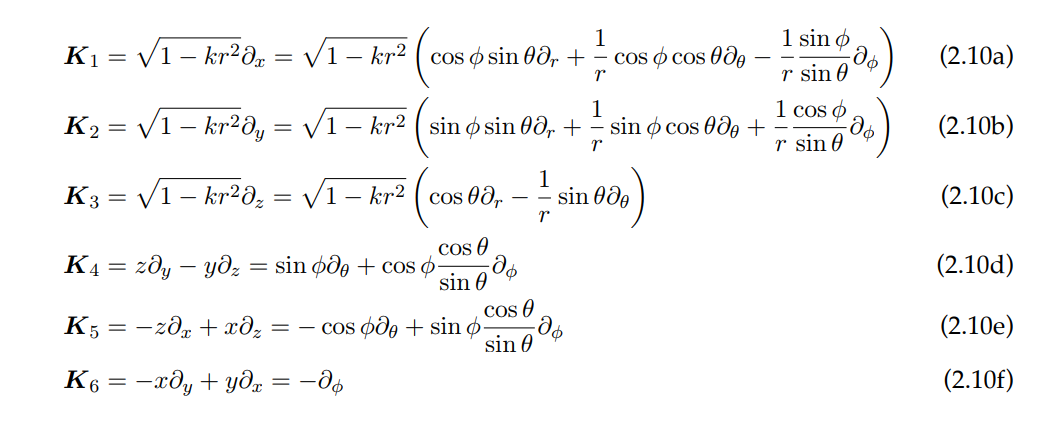
\includegraphics[width=0.7\linewidth]{gfx/CosmologyKillingVectorFields}
	\caption{}
	\label{fig:cosmologykillingvectorfields}
\end{figure}

in Cartesian and polar coordinates, respectively. The Killing condition \ref{eq:Killingeq}, iterated over
these six vector fields, then constitutes a set of partial differential equations for the components of the spacetime geometry tensor field $G$ in a choice of coordinates. Its solution
is, by definition, a tensor field that fulfills cosmological symmetries.

\begin{statements}
	Tracing the cosmological Killing vector fields foliates spacetime.
\end{statements}
We note here that the cosmological Killing vector fields give rise to a foliation of
our spacetime manifold in spatial hypersurfaces $Σ_t$ with a time parameter $t$ already. This
becomes apparent when we choose any point on the manifold and follow the integral
curves traced by the Killing vector fields that pierce through this point. Any two points on
the manifold connected by this procedure lie on the same spatial hypersurface. These vector
fields allow for a choice of chart where following any of their integral curves never
changes the coordinate we denoted as $w$ above and that we may now refer to as cosmic
time $t$. They still allow for reparametrizations $t → t^\prime$ of this coordinate however, that we
can describe through a lapse function $N(t)=\frac{\md t^\prime}{\md t}$.\\
Now with a set of Killing vector fields at hand that represent the cosmological symmetries, constructing a symmetric geometry reduces to the exercise of solving the Killing
condition \ref{eq:Killingeq} for it.\\
\\
The standard cosmological FLRW metric arises as the solution of the Killing condition \ref{eq:Killingeq}
for a Lorentzian metric geometry $g$
\begin{equation}
	0=K^m_i  \partial_m g^{ab} - 2 g^{m (a} \partial_m K^{b)}_i,
\end{equation}
where the $\mathbf{K}_i$ denote the six cosmological Killing vector fields as found above. This is a set of ten
partial differential equations for each of the six Killing vector fields. It is the Lie derivative \ref{eq:Killingeq} for a symmetric tensor field $g^{ab}$ written in components.
\\
\\
We choose a time coordinate and spatial polar coordinates $(t, r, θ, ϕ)$ to first solve the set
of equations for the metric components $g^{ab}$ and their derivatives $∂_mg^{ab}$, where we treat the $g^{ab}$ and $∂_mg^{ab}$ as independent variables. Solving the set of equations
then leaves only two metric components and both their derivatives by the time coordinate
undetermined. With these components chosen as $g_{tt}$ and $g_{rr}$, the remaining variables
solve to
\begin{figure}[h!]
	\centering
	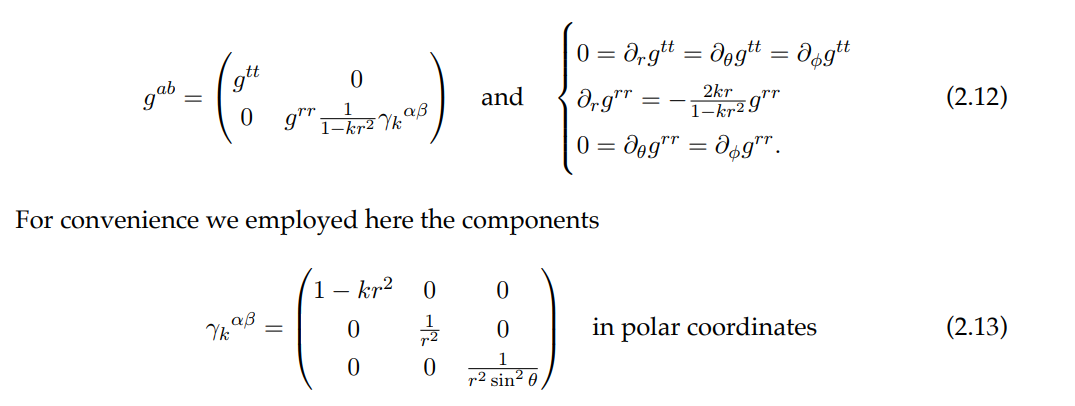
\includegraphics[width=0.7\linewidth]{gfx/FLRWmetricviaKilling}
	\caption{}
	\label{fig:flrwmetricviakilling}
\end{figure}
of a three dimensional Riemannian metric of constant curvature to abbreviate the notation. Note that we will also make use of its inverse $γ_{kαµ}γ^{k
µβ} = δ^\beta_α$
and its determinant $γ_k ≡ \det (
γ{kαβ})$.\\
\\
Now we are only left with solving the partial differential equations, in the figure the upper equations. They have
the solution
\begin{equation}
	g_{tt}=C_1(t) \qquad g_{rr} = -C_2(t) (1-kr^2)
\end{equation}
where two free functions $C_1(t)$ and $C_2(t)$ arise from the integration. Only the condition that the metric be Lorentzian constrains these functions, requiring that both be non-negative. To obtain a unique parametrization we therefore impose two conditions that
each define a metric degree of freedom:
\begin{enumerate}
	\item In a foliation of the spacetime manifold in spatial hypersurfaces we identify the
	lapse function
	\begin{equation}
		g^{tt} \stackrel{!}{=} \frac{1}{N^2(t)}.
	\end{equation}
	\item We compute the metric volume element
	\begin{equation}
\sqrt{-g} = N(t)C_2(t)^{-\frac{3}{2}}\sqrt{\gamma_k}
	\end{equation}
	and define a \emph{volume scale factor} $a(t)$ through the condition
	\begin{equation}
		\sqrt{-g}\stackrel{!}{=} N(t) a^3(t) \sqrt{\gamma_k}.
	\end{equation}
\end{enumerate}
Both conditions only serve to connect the arbitrary parametrization by $C_1(t)$ and $C_2(t)$ to
the conventional metric degrees of freedom $N(t)$ and $a(t)$ as
\begin{equation}
	C_1(t) = \frac{1}{N(t)} \quad and \quad C_2(t)=\frac{1}{a^2(t)}.
\end{equation}
With this choice of parameters we arrive precisely at the canonical FLRW metric
\begin{equation}
g^{ab} =
\begin{pmatrix}
\frac{1}{N^2(t)}&0\\
0& - \frac{1}{a^2(t)} \gamma^{\,\, \mu \nu}_k
\end{pmatrix}
\end{equation}
where indeed the scale factor $a(t)$ scales a three dimensional Riemannian metric of constant curvature $γ_k$. Note that in the literature the lapse function is usually chosen as $N(t) = 1$
in a particular choice of cosmic time.

\subsection{Conservation laws from Killing vector fields - More in depth}
Freely-falling particles and light rays both follow geodesics. For $\gamma$ a geodesic, then the projection of a Killing vector K on the tangent to the geodesic $\dot{\gamma}$ is constant along the geodesic,
\begin{equation}
\nabla_{\dot{\gamma}} \langle \dot{\gamma},K\rangle = 0.
\end{equation}
The constancy of $\langle \dot{\gamma},K\rangle$ along the geodesics means that each Killing vector field gives rise to a conserved quantity for freely-falling particles and light rays. Since a Killing vector field generates an isometry, this shows that 
\begin{statements}
	Symmetry transformations of the metric give rise to conservation laws.
\end{statements}

Killing fields are the infinitesimal generators of isometries; that is, flows generated by Killing fields are continuous isometries of the manifold  $\Leftrightarrow$ The flow generates a symmetry, in the sense that moving each point on an object the same distance in the direction of the Killing vector will not distort distances on the object.\\
E.g., in a \emph{static configuration}, in which nothing changes with time, the time vector will be a Killing vector, and thus the Killing field will point in the direction of forward motion in time.\\
\\
\\
A \emph{maximally symmetric space} is one
which possesses the largest possible number of Killing vectors, which on an $n$-dimensional
manifold is $n(n + 1)/2$. We will not prove this statement, but it is easy to understand at an
informal level. Consider the Euclidean space $\mR^n$ , where the isometries are well known to us:
translations and rotations. In general there will be $n$ translations, one for each direction we
can move. There will also be $n(n − 1)/2$ rotations; for each of $n$ dimensions there are $n − 1$
directions in which we can rotate it, but we must divide by two to prevent overcounting
(rotating $x$ into $y$ and rotating $y$ into $x$ are two versions of the same thing).
We therefore have
\begin{equation}
	n + \frac{n(n-1)}{2} = \frac{n(n+1)}{2}
\end{equation}
independent Killing vectors.
\subsection{Explicit Killing vectors}
For example in $\mR^2$ with metric $ds^2 = dx^2 +dy^2$ ,
independence of the metric components with respect to $x$ and $y$ immediately yields two
Killing vectors:
\begin{align}
	X^\mu &= (1,0) \nonumber \\
	Y^\mu &= (0,1) .
\end{align}
These clearly represent the two translations. The one rotation would correspond to the
vector $R = ∂/∂θ$ if we were in polar coordinates; in Cartesian coordinates this becomes
\begin{equation}
	R^{\mu} =(-y,x).
\end{equation}
These solve Killing's equation.\\
\\
Note that in $n ≥ 2$ dimensions, there can be more Killing vectors than dimensions. This
is because a set of Killing vector fields can be linearly independent, even though at any one
point on the manifold the vectors at that point are linearly dependent. It is trivial to show
(so you should do it yourself) that a linear combination of Killing vectors with constant
coefficients is still a Killing vector (in which case the linear combination does not count as
an independent Killing vector), but this is not necessarily true with coefficients which vary
over the manifold. You will also show that the commutator of two Killing vector fields is a
Killing vector field; this is very useful to know, but it may be the case that the commutator
gives you a vector field which is not linearly independent (or it may simply vanish).


















\section{Differential forms}
Differential $p$-forms are totally antisymmetric tensors of rank $(0,p)$.\\
The \emph{exterior product} $\wedge$ is defined by 
\begin{equation}
\wedge:\bigwedge^p \times \bigwedge^q \rightarrow \bigwedge^{p+q}, (\omega, \eta) \mapsto \omega \wedge \eta = \frac{(p+q)!}{p!q!} \mathcal{A}(\omega\otimes \eta),
\end{equation}
where $\mathcal{A}$ is the alternation operator
\begin{equation}
	(\mathcal{A}t)(v_1,\dots,v_p) = \frac{1}{p!} \sum_{\pi} \mathrm{sgn}(\pi) t(v_{\pi(1)}, \dots, v_{\pi(p)}).
\end{equation}
This operator we use to symmetrize or antisymmetrize tensors. To \emph{symmetrize}, we take the sum of all permutations of the relevant indices
and divide by the number of terms:
\begin{equation}
	T^{\sigma}_{(\mu_1 \dots \mu_n)\rho} = \frac{1}{n!} \left(T^{\sigma}_{\mu_1 \dots \mu_n \rho} + \mathrm{sum\,over\,permutations\,of\,indices\,} \mu_1 \dots \mu_n\right),
\end{equation}
while \emph{antisymmetrization} comes from the alternating sum:
\begin{equation}
T^{\sigma}_{[\mu_1 \dots \mu_n]\rho} = \frac{1}{n!} \left(T^{\sigma}_{\mu_1 \dots \mu_n \rho} + \mathrm{alternating\,sum\,over\,permutations\,of\,indices\,} \mu_1 \dots \mu_n\right).
\end{equation}
By “alternating sum” we mean that permutations which are the result of an odd number of
exchanges are given a minus sign, thus
\begin{equation}
	T_{[\mu \nu \rho] \sigma} = \frac{1}{6} \left[T_{\mu \nu \rho \sigma } - T_{\mu \rho \nu \sigma}  +T_{\rho \mu \nu  \sigma} -T_{\nu \mu \rho  \sigma} +T_{\nu \rho \mu \sigma}-T_{\rho \nu \mu \sigma} \right].
\end{equation}

On the vector space $\bigwedge$ of differential forms, the wedge product defines an \emph{associative, skew-commutative Grassman algebra},
\begin{equation}
	\omega \wedge \eta = (-1)^{pq} \eta \wedge \omega, \quad \omega \in \bigwedge^p, \eta \in \bigwedge^q.
\end{equation}
Given a $p$-form $A$ and a $q$-form $B$, we can form a $(p + q)$-form known as the wedge
product $A \wedge B$ by taking the antisymmetrized tensor product:
\begin{equation}
	(A\wedge B)_{\mu_1 \dots \mu_{p+q}} = \frac{(p+q)!}{p! q!} A_{[\mu_1 \dots \mu_p} B_{\mu_{p+1} \dots \mu_{p+1}]}.
\end{equation}
Thus, for example, the wedge product of two 1-forms is
\begin{equation}
	(A \wedge B)_{\mu \nu} = 2 A_{[\mu} B_{\nu]} = A_{\mu} B_{\nu} - A_{\nu} B_{\mu}.
\end{equation}



A basis for the $p$-forms is $\md x^{i_1} \wedge \dots \wedge \md x^{i_p}$, which shows that
\begin{equation}
	\dim{\bigwedge^p} = 
	\begin{pmatrix}
	n\\
	p
	\end{pmatrix}\qquad 
i \leq i_1 < \dots < i_p \leq n,
\end{equation}
where $\{\md x^i\}$ has $i\in \{1,\dots,n\}$ basis of $V^*$. So at a point on a 4-dimensional spacetime there is one linearly independent 0-form, four
1-forms, six 2-forms, four 3-forms, and one 4-form. There are no p-forms for p > n, since all
of the components will automatically be zero by antisymmetry.\\
\\
The \emph{interior product} $i_v$ is defined by 
\begin{equation}
	i:TM\times \bigwedge^p \rightarrow \bigwedge^{p-1}, (v,w) \mapsto i_v(w) =w(v,\dots) \Leftrightarrow (i_v w)_{i_2 \dots i_p} = v^j w_{j i_2 \dots i_p}.
\end{equation}
The \emph{exterior derivative} turns $p$-forms $w$ into $(p+1)$-forms $\md w$,
\begin{equation}
	\md : \bigwedge^p \rightarrow \bigwedge^{p+1}, \quad \omega \mapsto \md \omega = (p+1) \mathcal{A}(\nabla \omega).
\end{equation}
Thus, it also turns a $p$ tensor into a $(p+1)$ tensor, being unaffected of the curvature of our space. As it also formulated for the covariant derivative of tensors under the connection section, one can see this property by simply noting that the partial derivatives used to define the exterior derivative can be replaced with covariant derivatives, because the contribution of the affine connection coefficients that appear in the covariant derivatives vanish upon antisymmetrization.\\
Due to the symmetry of the Levi-Civita connection, the components of the exterior derivative are given by partial derivatives,
\begin{equation}
	(\md \omega)_{i_1,\dots,i_{p+1}} = (p+1) \partial_{[i_1} \omega_{i_2 \dots i_{p+1}]}.
\end{equation}
Equivalently with a use of basis,
\begin{align}
	\omega &= \omega_{i_1 \dots i_p} \md x^{i_1} \wedge \dots \wedge \md x^{i_p}, \\
	\md \omega &= \md \omega_{i_1 \dots i_p} \wedge \md x^{i_1} \wedge \dots \wedge \md x^{i_p},
\end{align}
where the differentials are wedged from the left. The simplest example is the gradient, which is the exterior derivative of a 1-form $(\md \phi)_{\mu} = \partial_{\mu}\phi$. The reason why the exterior derivative deserves special attention is that it is a tensor, even in
curved spacetimes, unlike its cousin the partial derivative.\\
Note that in general an exact $p$-form $t$ is not unique, given one such $t$, the most general $p$-form satisfying the exactness equation is of the form
\begin{equation}
	t^\prime = t + \md u \qquad u\in\bigwedge^{\quad \quad \quad (p-1)}.
\end{equation}
For instance, if the vector potential of the field strength tensor $F\munu$, hence $A_\alpha$, is one vector potential whose curl is $F_{\alpha \beta}$, then the most general such vector potential is given by the "gauge transformation":
\begin{equation}
	A^\prime_\alpha = A_\alpha + \partial_\alpha \Phi, \qquad \Phi \in \bigwedge^{\;\;0}.
\end{equation}





\subsection{Detour- de Rham Cohomology -- TO EXPAND}
We define a $p$-form $A$ to be \emph{closed} if $\md A = 0$,
and \emph{exact} if $A = \md B$ for some $(p − 1)$-form $B$. Obviously, all exact forms are closed, but the
converse is not necessarily true. On a manifold $M$, closed $p$-forms comprise a vector space
$Z^p (M)$, and exact forms comprise a vector space $B^p (M)$. Define a new vector space as the
closed forms modulo the exact forms:
\begin{equation}
	H^p(M) = \frac{Z^p(M)}{B^p(M)}.
\end{equation}
This is known as the \emph{$p$th de Rham cohomology vector space}, and depends only on the
topology of the manifold $M$. (Minkowski space is topologically equivalent to $\mR^4$ , which is
uninteresting, so that all of the $H^p (M)$ vanish for $p > 0$; for $p = 0$ we have $H^0 (M) = \mR$.
Therefore in Minkowski space all closed forms are exact except for zero-forms; zero-forms
can’t be exact since there are no $n$−1-forms for them to be the exterior derivative of.) It is
striking that information about the topology can be extracted in this way, which essentially
involves the solutions to differential equations. The dimension $b_p$ of the space $H^p (M)$ is
called the $p$th \emph{Betti number} of $M$, and the \emph{Euler characteristic} is given by the alternating
sum
\begin{equation}
	\chi(M) = \sum_{p=0}^{n} (-1)^p b_p.
\end{equation}
Cohomology theory is the basis for much of modern differential topology.



\subsection{Hodge star operator}
The  \emph{Hodge star operator} turns a $p$-form into an $(n-p)$- form,
\begin{equation}
	*:\bigwedge^p \rightarrow \bigwedge^{n-p}, \omega \mapsto * \omega,
\end{equation}
i.e. mapping $\omega$ to “$\omega$ dual”. Unlike our other operations on forms, the Hodge dual does depend
on the metric of the manifold (which should be obvious, since we had to raise some indices
on the Levi-Civita tensor in order to define it). Two facts on the Hodge dual: First, “duality” in the sense of Hodge is different than the
relationship between vectors and dual vectors, although both can be thought of as the space
of linear maps from the original space to $\mR$. Notice that the dimensionality of the space of
$(n − p)$-forms is equal to that of the space of $p$-forms, so this has at least a chance of being
true. In the case of forms, the linear map defined by an $(n − p)$-form acting on a p-form is
given by the dual of the wedge product of the two forms. Thus, if $A^{(n−p)}$ is an $(n − p)$-form
and $B^{(p)}$ is a $p$-form at some point in spacetime, we have
\begin{equation}
	*(A^{(n-p)}  \wedge B^{(p)}) \in \mR.
\end{equation}
The second fact concerns differential forms in 3-dimensional Euclidean space. The Hodge
dual of the wedge product of two 1-forms gives another 1-form:
\begin{equation}
	*(U\wedge V)_i = \epsilon^{\; jk}_i U_j V_k.
\end{equation}
(All of the prefactors cancel.) Since 1-forms in Euclidean space are just like vectors, we have
a map from two vectors to a single vector. You should convince yourself that this is just the
conventional cross product, and that the appearance of the Levi-Civita tensor explains why
the cross product changes sign under parity (interchange of two coordinates, or equivalently
basis vectors). This is why the cross product only exists in three dimensions — because only
in three dimensions do we have an interesting map from two dual vectors to a third dual
vector.
\\
\\
If $\{\md x^i\}$ is the basis of the dual space $T^*_p M$, then
\begin{equation}
	*(\md x^{i_1} \wedge \dots \wedge \md x^{i_p}) = \frac{\sqrt{|g|}}{(n-p)!} \epsilon^{i_1 \dots i_p}_{\quad \quad \quad i_{p+1} \dots i_n} \md x^{i_{p+1}} \wedge \dots \wedge \md x^{i_n},
\end{equation}
where the Levi-Civita tensor is only covariantly defined, i.e. $\epsilon_{i_1 \dots i_p} = \pm 1$ and indices have to be pushed up by $g^{\mu \nu} = (g_{\mu \nu})^{-1}$.
Here you symmetrize if the components are not in perfect order, i.e. for $\{x^0=c t ,r,\vartheta, \varphi\}$ one has
\begin{equation}
	*(\md \vartheta \wedge \varphi) = \frac{\sqrt{\abs{g}}}{(4-2)!} \left[\epsilon^{\vartheta \varphi}_{ct,r} c \md t\wedge \md r + \epsilon^{\vartheta \varphi}_{r,ct} \md r\wedge c\md t\right]=\frac{c \md t \wedge \md r}{r^2 \sin\vartheta}.
\end{equation}\\
For the orthonormal basis $\{e^i\}$ of $TM$,
\begin{equation}
	*(e^{i_1} \wedge\dots \wedge e^{i_p}) = e^{i_{p+1}} \wedge \dots \wedge e^{i_n}.
\end{equation}
As an intriguing aside, Hodge duality is the basis for one of the hottest topics in theoretical
physics today. It’s hard not to notice that the equations 
\begin{equation}
\md F = 0
\end{equation}
and 
\begin{equation}
\md (*F) = 4 \pi (* J)
\end{equation} look very similar.
Indeed, if we set $J_μ = 0$, the equations are invariant under the “duality transformations”
\begin{align*}
	F &\rightarrow *F\\
	*F & \rightarrow -F.
\end{align*}
We therefore say that the vacuum Maxwell’s equations are duality invariant, while the invariance is spoiled in the presence of charges. We might imagine that magnetic as well as electric monopoles existed in nature; then we could add a magnetic current term $4π(∗J_M )$ to the
right hand side of $\md F=0$, and the equations would be invariant under duality transformations
plus the additional replacement $J ↔ J_M$ . Long
ago Dirac considered the idea of magnetic monopoles and showed that a necessary condition
for their existence is that the fundamental monopole charge be inversely proportional to the fundamental electric charge. Now, the fundamental electric charge is a small number;
electrodynamics is “weakly coupled”, which is why perturbation theory is so remarkably
successful in quantum electrodynamics (QED). But Dirac’s condition on magnetic charges
implies that a duality transformation takes a theory of weakly coupled electric charges to a
theory of strongly coupled magnetic monopoles (and vice-versa). Unfortunately monopoles
don’t exist (as far as we know), so these ideas aren’t directly applicable to electromagnetism;
but there are some theories (such as supersymmetric non-abelian gauge theories) for which
it has been long conjectured that some sort of duality symmetry may exist. If it did, we
would have the opportunity to analyze a theory which looked strongly coupled (and therefore
hard to solve) by looking at the weakly coupled dual version. Recently work by Seiberg and
Witten and others has provided very strong evidence that this is exactly what happens in
certain theories. The hope is that these techniques will allow us to explore various phenom-
ena which we know exist in strongly coupled quantum field theories, such as confinement of
quarks in hadrons.


\subsection{Codifferential}
The \emph{codifferential} is a differentiation lowering the order of a $p$-form by one,
\begin{equation}
	\delta:\bigwedge^p \rightarrow \bigwedge^{p-1},\; \omega \mapsto \delta \omega = \mathrm{sgn}(g)\; (-1)^{n(p+1)} (*\md *)(\omega).
\end{equation}
It generalises the divergence:
\begin{equation}
	(\delta \omega)^{i_1 \dots i_{p-1}} = \frac{1}{\sqrt{|g|}} \partial_k \left(\sqrt{|g|} \omega_{k i_1 \dots i_{p-1}}\right).
\end{equation}


\subsection{Conventional differential operators via forms}
How can the exterior derivative and the co-differential be used to express the conventional
differential operators on vector fields, i.e. the curl, the divergence, and the Laplacian?\\
If $ω$ is the 1-form that belongs to the vector field $v$, i.e. $ω = v^{\flat} ∈ \bigwedge^{\;\;1}$ , its curl is given by $∗\md ω$,
i.e. the Hodge dual of the external derivative
\begin{equation}
	\mathrm{curl}\omega=*\md\omega, \quad \mathrm{curl} v=\left(*\md v^\flat\right)^\sharp.
\end{equation}
 The divergence of $ω$ is given by $δω$, i.e. the
co-differential:
\begin{equation}
	\mathrm{div}\omega=\nabla^\mu \omega_\mu = \delta \omega \quad \nabla_a\omega_b=\abs{g}^{-\half} \partial_a\left(\sqrt{\abs{g}} \omega_b\right),
\end{equation} 
or 
\begin{equation}
	\mathrm{div} v= \left(\delta v^\flat\right)^\sharp.
\end{equation}
The Laplacian of $ω$ is given by the Laplace-de Rham operator 
\begin{equation}
	\Delta \omega = (\md \circ \delta + \delta \circ \md) \omega,
\end{equation}
or
\begin{equation}
	\Delta v=\left[(\md \circ \delta + \delta \circ \md ) v^\flat\right]^\sharp.
\end{equation}
Then, for a function like the pressure $p$, one has
\begin{equation}
	g^{μα} ∇_α p = g^{μα} ∂_α p = g^{μα} (\md p)_α = (dp^\sharp)_μ = (\grad p)_μ .
\end{equation}








\section{Integrals}
The \emph{canonical volume form} on a pseudo-Riemannian manifold $(M,g)$ is defined by
\begin{equation}
	\eta = \sqrt{|g|} \md x^1 \wedge \dots \wedge \md x^n \quad \in \bigwedge^n.
\end{equation}
The integration of $n$-forms $\omega=f(x_1,\dots,x_n) \md x^1 \wedge \dots \wedge \md x^n$ over domains $D\subset M$ is coordinate independent and defined by
\begin{equation}
	\int_D \omega = \int_D f(x_1, \dots, x_n) \md x^1 \wedge \dots \wedge \md x^n.
\end{equation}
$\Rightarrow$ Functions $f$ are integrated by means of the canonical volume form,
\begin{equation}
	\int_D f \eta =\int_D f \sqrt{|g|} \md x^1 \wedge \dots \wedge \md x^n.
\end{equation}
\begin{mybox}{Stokes' theorem}
	Let $M$ be an $n$-dimensional manifold and the region $D\subset M$ have a smooth boundary $\partial D$ such that $\bar{D} = D \cup \partial D$ is compact. Then, for every $(n-1)$-form $\omega$, we have 
	\begin{equation}
		\int_D \md \omega = \int_{\partial D} \omega.
	\end{equation}

\end{mybox}

\begin{mybox}{Gauss' theorem}
	Likewise, for a vector field $X\in TM$ on $M$ and $x^{\flat}$ the 1-form belonging to this vector field:
	\begin{equation}
	\int_D \delta x^{\flat} \eta = \int_{\partial D} *x^{\flat}.
	\end{equation}
\end{mybox}

The musical operators used here are isomorphisms between the tangent spaces of a manifold and their dual spaces given by the metric
\begin{equation}
	\flat : TM \rightarrow T^*M, v \mapsto v^{\flat}, v^{\flat}_i =g_{ij} v^j,
\end{equation}
and similarly by the inverse of the metric,
\begin{equation}
	\#:T^*M \rightarrow TM, \omega \mapsto \omega^{\#}, \; (\omega^{\#})^i = g^{ij} \omega_j.
\end{equation}
Like $\flat$ lowers a note by a semitone in music, the $\flat$ operator lowers the index of vector components and thus turns then into dual vector components.. Analogously, $\#$ raises notes by semitones in music, and indices of dual-vector components.




\section{Frame fields in GR and the Tetrad formalism, "tetrad"="vierbein"="frame field"}
The tetrad formalism is an approach to general relativity that generalizes the choice of basis for the tangent bundle from a coordinate basis to the less restrictive choice of a local basis, i.e. a locally defined set of four linearly independent vector fields called a \emph{tetrad}.\\
The tetrad basis is chosen: a set of four independent vector fields
\begin{equation}
	e_a = e^{\mu}_a \partial_{\mu}, \quad \mathrm{for} \quad a=0,1,2,3,
\end{equation}
hat together span the 4D vector tangent space at each point in spacetime. Note that $e_0$ is a timelike vector field and $e_i$ is a spacelike vector field. Dually, a tetrad determines (and is determined by) a dual co-tetrad—a set of four independent covectors (1-forms)
\begin{equation}
	\theta^a = \theta^a_{\mu} \md x^{\mu}, \quad \theta^a \equiv e^a,
\end{equation}
such that $\theta^a(e_b) = \theta^a_{\mu} \theta^{\mu}_b=e^a_{\mu} e^{\mu}_b = \delta^a_b$.
A tetrad is specified by its coefficients $e^{\mu}_a$ w.r.t. a coordinate basis, despite the fact that the choice of a tetrad does not actually require the additional choice of a set of (local) coordinates $x^{\mu}$.\\
\\
In the tetrad formalism, all tensors are represented i.t.o. a chosen basis, vector or covector basis, by expressing them as linear combinations of numbers of the (co)tetrad. Popular tetrad bases include orthonormal tetrads and null tetrads, where the latter are composed of four null vectors (used in radiation problems).
\\
\\
Physical interpretation:\\
\textbf{Frame fields always correspond to a family of ideal observers immersed in the given spacetime; the integral curves of the timelike unit vector field are the worldlines of these observers, and at each event along a given worldline, the three spacelike unit vector fields specify the spatial triad carried by the observer. The triad may be thought of as defining the spatial coordinate axes of a local laboratory frame, which is valid very near the observer's worldline.}\\

In general, the worldlines of these observers need not be timelike geodesics. If any of the worldlines bends away from a geodesic path in some region, we can think of the observers as test particles that accelerate by using ideal rocket engines with a thrust equal to the magnitude of their acceleration vector. Alternatively, if our observer is attached to a bit of matter in a ball of fluid in hydrostatic equilibrium, this bit of matter will in general be accelerated outward by the net effect of pressure holding up the fluid ball against the attraction of its own gravity. Other possibilities include an observer attached to a free charged test particle in an electrovacuum solution, which will of course be accelerated by the Lorentz force, or an observer attached to a spinning test particle, which may be accelerated by a spin–spin force.\\

It is important to recognize that frames are geometric objects. That is, vector fields make sense (in a smooth manifold) independently of choice of a coordinate chart, and (in a Lorentzian manifold), so do the notions of orthogonality and length. Thus, just like vector fields and other geometric quantities, frame fields can be represented in various coordinate charts. Computations of the components of tensorial quantities, with respect to a given frame, will always yield the same result, whichever coordinate chart is used to represent the frame.\\
\\ 
The standard formalism of GR consists simply of using the coordinate tetrad in the tetrad formalism. The coordinate tetrad is the canonical set of vectors associated with the coordinate chart and is commonly denoted $\{\partial_{\mu}\}$, whereas the dual cotetrad is denoted $\{\md x^{\mu} \}$.\\
In the tetrad formalism, instead of writing tensor equations out fully (including $e_a,\theta^a$ and $\otimes$) only components of the tensors are mentioned, e.g. the metric is written as "$g_{ab}$".\\
\\
Changing tetrads is a routine operation in the standard formalism, as it is involved in every coordinate transformation (i.e., changing from one coordinate tetrad basis to another). Switching between multiple coordinate charts is necessary because, except in trivial cases, it is not possible for a single coordinate chart to cover the entire manifold. Changing to and between general tetrads is much similar and equally necessary (except for parallelizable manifolds). Any tensor can locally be written in terms of this coordinate tetrad or a general (co)tetrad. For example, the metric can be written as
\begin{equation}
	g=g_{\mu \nu} \md x^{\mu} \md x^{\nu}, \quad \mathrm{where} \quad g_{\mu \nu} = g(\partial_{\mu},\partial_{\nu}).
\end{equation}
For an arbitrary cotetrad (use $e^a \equiv \theta^a$ dual to $e_a$)
\begin{equation}
	g=g_{ab} e^a e^b, \qquad \mathrm{where} \quad g_{ab} = g(e_a,e_b).
\end{equation}
We can translate from a general co-tetrad to the coordinate co-tetrad by expanding the covector
\begin{align*}
	e^a &= e^a_{\mu} \md x^{\mu},\\
	\Rightarrow g=g_{ab}e^a e^b = g_{ab} e^a_{\mu} e^b_{\nu} \md x^{\mu} \md x^{\nu} &\stackrel{!}{=} g_{\mu \nu} \md x^{\mu} \md x^{\nu} \\
	\Leftrightarrow g_{\mu \nu} &= g_{ab} e^a_{\mu} e^b_{\nu}.
\end{align*}
Likewise expanding $\md x^{\mu}=e^{\mu}_a e^a$ w.r.t. the general tetrad, we get
\begin{align*}
	g&= g_{\mu \nu} \md x^{\mu} \md x^{\nu} = g_{\mu \nu} e^{\mu}_a e^a e^{\nu}_b e^b \\
	&=g_{ab} e^a e^b \\
	\Leftrightarrow g_{\mu \nu} e^{\mu}_a e^{\nu}_b &=g_{ab}.
\end{align*}
Be \emph{careful}:\\
The manipulation with tetrad coefficients shows that abstract index formulas can, in principle, be obtained from tensor formulas with respect to a coordinate tetrad by "replacing greek by latin indices". However care must be taken that a coordinate tetrad formula defines a genuine tensor when differentiation is involved. Since the coordinate vector fields have vanishing Lie bracket (i.e. commute: $ \partial_{\mu} \partial_{\nu} =\partial_{\nu} \partial_{\mu}$ ), naive substitutions of formulas that correctly compute tensor coefficients with respect to a coordinate tetrad may not correctly define a tensor with respect to a general tetrad because the Lie bracket is non-vanishing:$[e_a,e_b]\neq 0$.\\
E.g:
\begin{equation}
	\bar{R}(X,Y) =\left(\nabla_X \nabla_Y - \nabla_Y \nabla_Y - \nabla_{[X,Y]} \right),
\end{equation}
in a coordiante tetrad this gives the tensor coefficients
\begin{equation}
	\bar{R}^{\mu}_{\nu \sigma \tau} = \md x^{\mu} \left[\left(\nabla_{\sigma} \nabla_{\tau} - \nabla_{\tau} \nabla_{\sigma}\right) \partial_{\nu}\right].
\end{equation}
The naive and  "greek to latin" substitution of this is 
\begin{equation}
	\bar{R}^a_{bcd} = e^a\left[\left(\nabla_c \nabla_d - \nabla_d \nabla_c\right)e_b\right],\quad \mathrm{WRONG}
\end{equation}
is \emph{incorrect} because for fixed $c$ and $d$, $\left(\nabla_c \nabla_d - \nabla_d \nabla_c\right)$ is a first order differential operator rather than a zeroth order operator which defines a tensor coefficient. Substituting a general tetrad basis, we find the proper definition of $\bar{R}$ in abstract index notation:
\begin{equation}
	\bar{R}^a_{bcd} = e^a\left[\left(\nabla_c \nabla_d - \nabla_d \nabla_c - f^{\;\; e}_{cd} \nabla_e\right) e_b\right],
\end{equation}
where $\left[e_a,e_b\right]=f^{\; \; c}_{ab} e_c$.
\\
\\
Abstract index notation: $V$ a vector space, then for $(2,0)$-tensor $h \in V^* \otimes V^*$, or also
\begin{equation}
	\bar{R} = \bar{R}^{\; \; \; d}_{abc} \in \left(V^* \otimes V^* \otimes V^* \otimes V\right),
\end{equation}
therefore representing how covariant indices,i.e. $d$, represent the tensor swallowing one dual-vector (since $V$) and the contravariant indices, i.e. $a,b,c$, represent the tensor swallowing three vectors (since $V^* \otimes V^* \otimes V^*$).
\subsection{On the tetrad formalism - Weinberg}
The method employed by general covariance to port theories from SR to GR actually works only for objects that behave like tensors under Lorentz transformation, and not for the spinor fields. (Mathematically, this is because the tensor representation of the group GL(4) of general linear $4\times4$ matrices behave like tensors under the subgroup of Lorentz transformations, but there are no representations of GL(4), or even "representations up to a sign", which behave like spinors under the Lorentz subgroup.) How then can we incorporate spinors into GR?\\
The answer lies in a different approach to the problem of determining the effects of gravitation on physical systems.\\
To start, let us take advantage of the Principle of Equivalence, and at every point $X$ erect a set of coordinates $\xi^\alpha_X$ that are locally inertial at $X$. (Of course, it will not be possible to erect any \emph{single} coordinate system that is locally inertial everywhere, unless the space-time continuum is "flat".) The metric in any general noninertial coordinate system is then
\begin{equation}
g\munu (x)  = V^\alpha_\mu(x) V^\beta_\nu(x) \eta_{\alpha \beta}
\end{equation}
where 
\begin{equation}
	V^\alpha_\mu(X) \equiv \left(\frac{ \partial \xi^\alpha_X(x)}{\partial x^\mu}\right)_{x=X}.
\end{equation}
\marginpar{Note that in our formalism, this is equivalent to the expansions: $V^\mu= V^\mu_a \theta^a$ or $V_\mu = V^a_\mu e_a$.}
Note that we fix the locally inertial coordinates $\xi^\alpha_X$ once and for all at each physical point $X$, so when we change our general noninertial coordinates from $x^\mu$ to $x^{\prime \mu}$, the partial derivatives $V^\alpha_\mu$ change according to the role
\begin{equation}
	V^\alpha_\mu \rightarrow V^{\prime \alpha}_\mu = \frac{\partial x^\nu}{\partial x^{\prime \mu}} V^\alpha_\nu.
\end{equation}
Thus, we are to think of $V^\alpha_\mu$ as forming \emph{four} covariant vector fields, \emph{not} as a single tensor: This set of four vectors is known as a \emph{tetrad}, or \emph{vierbein}.
\begin{mybox}{Why are we changing to tetrad basis, my interpretation}
	Thus, The change to the tetrad basis is the change to a locally inertial system, i.e. to a freely falling system (RNC) where space appears to be flat. This basis generally depends on the coordinates from before, such that the basis changes from point to point on the manifold, thus this doesn't violate principle of equivalence as it is not one basis for all of the manifold but a smoothly changing basis, i.e. it is adapted to the manifold such that everything always looks flat/freely falling.
\end{mybox}
Now, given any contravariant vector field $A^\mu(x)$, we can use the tetrad to refer to its components at $x$ to the coordinate system $\xi^\alpha_X$ locally inertial at $x$:
\begin{equation}
	A^\alpha \equiv V^\alpha_\mu A^\mu.
\end{equation}
We are contracting a contravariant vector $A^\mu$ with four covariant vectors $V^\alpha_\mu$, so this has the effect of replacing the single four-vector $A^\mu$ with the four scalar $A^\alpha$. For general tensors:
\begin{equation}
	B^\alpha_\beta \equiv V^\alpha_\mu V^\nu_\beta B^\mu_\nu,
\end{equation}
here $V^\nu_\beta$ is just the tetrad, but with $\alpha$-index lowered with the Minkowski tensor and $\mu$-index raised with the metric tensor:
\begin{equation}
	V^\nu_\beta \equiv \eta_{\alpha \beta}g^{\mu \nu} V^\alpha_\mu.
\end{equation}
Note that the different bases are orthogonal
\begin{equation}
	\delta^\mu_\nu = V^\mu_\beta V^\beta_\nu, \qquad \delta^\alpha_\beta=V^\alpha_\mu V^\mu_\beta.
\end{equation}
The scalar components of the metric tensor are then simply:
\begin{equation}
	g_{\alpha \beta} \equiv V^\mu_\alpha V^\nu_\beta g\munu = \eta_{\alpha \beta}
\end{equation}
\subsubsection{Constructing an action - TO DO for QFT on curved spacetime }
How would we construct an action if we worked from the beginning with the scalars $V^\alpha,T_{\alpha\beta}$. There are now \emph{two} invariance principles which must be met in constructing a suitable matter action $S_M$:
\begin{enumerate}
	\item The action must be generally covariant, with all fields treated as scalars, except for the tetrad itself.
	\item The Principle of Equivalence requires that special relativity should apply in locally inertial frames, and in particular, that it should make no difference which locally inertial frame we choose at each point. Thus since our scalar field components $V^\alpha,T_{\alpha \beta}..$ are defined w.r.t. an arbitrarily chosen locally inertial coordinate system, the field equations and the action must be invariant w.r.t. a redefiniton of thee locally inertial coordinate systems at each point, or in other words, w.r.t. Lorentz transformations $\Gamma^\alpha_\beta(x)$ that can depend on position in space-time. The tetrad changes according to the same rules:
	\begin{equation}
		V^\alpha_\mu(x)\rightarrow\Gamma^\alpha_\beta(x) V^\beta_\mu(x).
	\end{equation}
	For an arbitrary field $\psi_n(x)$ given in tetrad formalism
	\begin{equation}
	\label{eq:Lorentzspinor}
		\psi_n(x) \rightarrow \sum_m [D(\Gamma(x))]_{nm} \psi_m(x)
	\end{equation}
	where $D(\Gamma)$ is a matrix representation of the Lorentz group (or at least of the infinitesimal Lorentz group).
\end{enumerate}
These two invariance principles lead to a dual classification of physical quantities. A \emph{coordinate scalar} or \emph{coordinate tensor} transforms as a scalar or tensor under changes in the coordinate system. A \emph{Lorentz scalar} or \emph{Lorentz tensor} or \emph{Lorentz spinor} transforms according to \ref{eq:Lorentzspinor}, with $D(\Lambda)$ the identity or a tensor representation or a spinor representation of the infinitesimal Lorentz group, under changes in the choice of the locally inertial coordinate frame. For instance, a field such as $A^\alpha = V^\alpha_\mu A^\mu$ is a coordinate scalar and a Lorentz vector, the Dirac field of the electron is a coordinate scalar and a Lorentz spinor, and the tetrad $V^\alpha_\mu$ is a coordinate vector and a Lorentz vector. To be physically acceptable, the matter action $S_M$ must be both a coordinate scalar and a Lorentz scalar.\\
\\
How is the gravitational field going to get into this sort of theory, when the coordinate-scalar components of the $g_{\alpha \beta}=\eta_{\alpha \beta}$ of the metric tensor are just the constants $\eta_{\alpha \beta}$?
\begin{mybox}{HOW GRAVITY APPEARS IN A THEORY - IMPORTANT}
	\emph{The answer is that gravitational tensor fields appear in the action because, and only because, of the necessity of introducing} \textbf{derivatives} \emph{into the theory.}
\end{mybox}
If it made sense to construct an action $S_M$ solely from fields, and not their derivatives, then it would only be necessary to choose some arbitrary Lorentz-invariant function $\mL(\psi(x))$ of various fields $\psi_n(x)$ (but not the tetrad), call them all coordinate scalars, and take the action as 
\begin{equation}
	S_M = \int \md^4 x \sqrt{g(x)} \mL(\psi(x)).
\end{equation}
This would then automatically be a coordinate scalar and a Lorentz scalar.
\begin{mybox}{Construction of a gravitational action}
	However, we saw in \ref{ch:GRtheory} that any physically sensible action must involve derivatives of physical quantities as well as the quantities themselves.
\end{mybox}
The tetrad field must enter into the action in such a way as to keep it a coordinate scalar and a Lorentz scalar despite the presence of derivatives.
\\
\\
\begin{mybox}{How to go over to QFT on curved background via tetrad formalism}
	Only summarizing here:\\
	The effects of gravitation on any physical system can be taken into account by writing down the matter action or the field equations that hold in special relativity, and then replacing all derivatives $\partial/\partial x^\alpha$ with the "covariant derivatives"
	\begin{equation}
	\mathcal{D}_\alpha \equiv V_\alpha^\mu \frac{\partial}{\partial x^\mu} + \half  \sigma^{\beta \gamma} V^\nu_\beta V^\mu_\alpha V_{\gamma \nu;\mu},
	\end{equation}
	where the $\sigma$ matrices are the ones appearing for infinitesimal Lorentz trafos 
\end{mybox}
\todo{Make a section on Lorentz group, trafos and infinitesimal Lorentz trafos as well as generators}
\todo{Make a section on QFT on curved background including the spin connection in modern fashion, via tetrad formalism}
This prescription yields a matter acction or fields equations that are invariant under general coordinate transformations, with $V^\mu_\alpha$ regarded as a four-vector and with all other fields regarded as scalar, and that aslo do not depend on how we choose locally inertial frames in defining the tetrad.\\
\\
How does one define the energy-momentum tensor in this formalism ?
The variation $\delta V^\mu_\alpha$ in the tetrad field will produce in the matter action a change:
\begin{equation}
	\delta I_M = \int \md^4 x \sqrt{g} U^\alpha_\mu \delta V^\mu_\alpha
\end{equation}
where $U^\alpha_\mu$ is a coordinate vector and a Lorentz vector.
\\
Define the energy-momentum tensor by
\begin{equation}
\label{eq:energymomentumTetradformalism}
T\munu \equiv V_{\alpha \mu} U^\alpha_\nu.
\end{equation}
As required, this is manifestly a coordinate tensor and a Lorentz scalar. To verify that \ref{eq:energymomentumTetradformalism} is a suitable energy-momentum tensor, we must also check that it is symmetric and that it is covariantly conserved. The symmetry property of the energy-momentum tensor is not at all obvious in the tetrad formalism, but must be derived from the invariance of the matter action under the infinitesimal Lorentz transformations (also under position dependent ones). To show that this energy-momentum tensor is conserved, one uses the invariance of the matter action under infinitesimal coordinate transformations. This definition therefore works.\\
Note however, that if the matter action were not invariant under position-dependent Lorentz transformations, then not only would $T\munu$ not be symmetric, but in consequence, it would also not be conserved. One again construct the total action for matter and gravitation 
\begin{equation}
	S=S_M+S_G
\end{equation}
and gets the field equations from them. These equations serve to determine only $g\munu$, leaving the tetrad determined only up to a Lorentz transformation. However, the invariance of the matter action under such position-dependent Lorentz transformations ensures that all tetrads associated with a given metric have the same physical effects.

\section{Cartan's structure equations}
Let $M$ be a differentiable manifold, $\{e_i\}$ an arbitrary basis for vector fields and $\{\theta^i\}$ an arbitrary basis for dual vector fields, or 1-forms, such that 
\begin{equation}
	\langle \theta^i,e_j\rangle = \delta^i_j.
\end{equation}
\begin{mybox}{Connection forms}
	In analogy to $\Gamma^i_{jk}$, we introduce the connection forms $\omega^j_i$ by
	\begin{equation}
		\nabla_v e_a = \omega^b_a(v) e_b.
	\end{equation}
	Since $\nabla_v e_i$ is a vector, $\omega^j_i(v) \in \mR$, and thus $\omega^j_i \in \bigwedge^1$ is a dual vector, or a one form.
\end{mybox}
\marginpar{The connection forms are sometimes referred to as spin connection, which comes from the fact that this can be used to take covari-
	ant derivatives of spinors, which is actually impossible using the conventional connection
	coefficients.}
\begin{align}
	\nabla_{\partial_k} \partial_j &=\Gamma^i_{kj} \partial_i = \omega^i_j(\partial_k)\partial_i \nonumber \\
	\Rightarrow \omega^i_{\;j} &= \Omega^i_{kj} \md x^k \quad \Leftrightarrow \quad \omega^i_{\;j} = \Gamma^i_{kj} \theta^k.
\end{align}
\marginpar{Where one uses in $\{e_i\}$, $\omega_{ij} \equiv g_{ik} \omega^k_{\;j}, \quad g_{ij} = g(e_i,e_j)$.}
They satisfy the antisymmetry relation, if and only if $\nabla g=0$ the connection is metric:
\begin{equation}
	\md g_{ij} = \omega_{ij} + \omega_{ji}.
\end{equation}
The covariant derivative of a dual basis vector is
\begin{align}
	\nabla_v \theta^i &= - \omega^i_{\;j} (v) \theta^i,\\
	\nabla \theta^i &= - \theta^j \otimes \omega^i_{\;j}.
\end{align}
Covariant derivatives of arbitrary vector $x=x^i e_i$ and dual vector $\alpha=\alpha_j \theta^j$ are then
\begin{equation}
	\nabla_v x = \langle \md x^i + x^j \omega^i_{\;j}, v\rangle e_i, \quad \nabla_v \alpha = \langle \md \alpha_i - \alpha_j \omega^j_{\; i},  v\rangle \theta^i,
\end{equation}
or
\begin{equation}
	\nabla x = e_i \otimes \langle \md x^i+x^j \omega^i_{\;j}\rangle, \quad \nabla \alpha = \theta^i \otimes (\md \alpha_i - \alpha_k \omega^k_{\;i}).
\end{equation}
\marginpar{In QFT, the connection forms are the field strengths $F_{\mu \nu} \Leftrightarrow$ curvature forms. All this translates to structure of gauge theories. See chapter 2.}

\begin{mybox}{Torsion and curvature form}
	The torsion $T(x,y)$ is a vector, which can be written in terms of the torsion forms $\Theta^i$ as 
	\begin{equation}
		T(x,y) = \Theta^i(x,y) e_i, \quad \Theta^i \in \bigwedge^2 \quad \Rightarrow \; \Theta^i(x,y) \in \mR.
	\end{equation}
	Similarly, express the curvature by the curvature forms $\Omega^i_{\; j} \in \bigwedge^2$,
	\begin{equation}
		\bar{R}(x,y)e_j = \Omega^i_{\;j}(x,y)e_i.
	\end{equation}
\end{mybox}

\begin{mybox}{Cartan's structure equations}
	In terms of the connection forms $\omega^i_{\; j}$. the torsion forms $\Theta^i$ and the curvature forms $\Omega^i_{\;j}$ are determined by Cartan's structure equations,
	\begin{align}
		\label{eq:cartanStructure}
		\Theta^i &= \md \theta^i + \omega^i_{\;j} \wedge \theta^j,\\
		\Omega^i_{\;j} &= \md \omega^i_{\;j} + \omega^i_{\;k} \wedge \omega^k_{\; j}.
	\end{align}
\end{mybox}
\begin{mybox}{Computing the curvature tensors}
	The Riemann tensor in components is then obtained via
	\begin{equation}
		\bar{R}^a_{bcd} = \Omega^a_b(e_c,e_d)
	\end{equation}
	such that the Ricci tensor is given by the contraction of the first and third component
	\begin{equation}
		R_{bc} = \Omega^a_b(e_a,e_c).
	\end{equation}
	The torsion tensor is given by
	\begin{equation}
		T^a_{bc} = \Theta^a (e_b,e_c).
	\end{equation}
\end{mybox}
In reading off the connection forms, always think of antisymmetrizing the form such that
\begin{equation} 
	\md g_{ab} =0 =\omega_{ab}+\omega_{ba} 
\end{equation}
holds. That is, use the antisymmmetrizer in reading the connection forms off:
\begin{equation}
	(\omega \wedge \eta)=\frac{(p+q)!}{p!q!} \mathcal{A}(\omega\otimes\eta)
\end{equation}
such that for example
\begin{equation}
	(\theta^i\wedge \theta^j)(e_a,e_b) =\left[\theta^i(e_a) \theta^j(e_b) - \theta^i(e_b) \theta^j(e_a)\right].
\end{equation}
The components of the torsion and curvature tensors are determined by 
\begin{align}
	\Theta^i &= \frac{1}{2} T^i_{jk} \theta^j \wedge \theta^k,\\
	\Omega^i_{\;j} &= \frac{1}{2}  \bar{R}^i_{jkl} \theta^k \wedge \theta^l.
\end{align}
Note that the connection forms obtained from Cartan's structure equations have to be antisymmetrized in $i,j$ to get the full connection form. ALWAYS CHECK. This antisymmetry comes about by the metric being Minkowskian. Constant form of the metric here implies that we always can raise and lower indices by simply introducing minus or plus signs where appropriate
\begin{equation*}
	A^i_{\;\;j} = \pm A^{\;\; j}_i.
\end{equation*}
\\
\bullet Normally we have connection forms without torsion, will require that it has to vanish.
$\stackrel{Cartan}{\Rightarrow} \md \theta^i = - \omega^i_{\;k} \wedge \theta^i \Rightarrow$ choose a dual basis $\theta^i$, take derivative and read off $\omega^i_k$.\\
Recipe:\\
Introduce basis such that $g_{ij}=\pm 1\Rightarrow \md g_{ij} = 0 = \omega_{ij}+\omega_{ij} \Rightarrow$ only $6 \omega_{ij}$ left $ \Rightarrow$ easy calculation vs $\Gamma^i_{jk}\Rightarrow$ Minkowskian calculation with 
\begin{equation}
	g = g_{\mu \nu} \md x^{\mu} \otimes \md x^{\nu} = \tilde{g}_{\mu \nu} \theta^{\mu} \otimes \theta^{\nu},
\end{equation}
choose $\theta^{\mu},\theta^{\nu}$ such that $\tilde{g}_{\mu \nu} = \pm 1$. With this choice, the metric has become Minkowskian.
\begin{mybox}{Geodesic equation in tetrad formalism}
	The geodesic equation in the tetrad formalism reads
	\begin{equation}
		0=\nabla_u u = u^a \omega^{\;\;b}_a (u) e_b + u(u^b) e_b.
	\end{equation}
	Now you can project vectors $\theta^c$ onto this equation to find the different components $c \in \{0,1,2,3\}$.
	\begin{equation}
		u(u^a) + u^b \omega^a_b (u)=0.
	\end{equation}
\end{mybox}
\begin{mybox}{How to change basis}
	Consider a vector being given in coordinate tetrad and wanting to find the corresponding vector in the corresponding general tetrad:
	\begin{equation}
		u=\tilde{u}^\mu \partial_\mu = u^a e_a.
	\end{equation}
	The components are then given by
	\begin{equation}
		u^0 = \theta^0(u) = \tilde{u}^0 \theta^0(\partial_0) + \tilde{u}^i \theta^0(\partial_i).
	\end{equation}
	The orthonormality of the two different tetrad basis $\partial_i$ and co-basis $\theta^a$ is not guaranteed. Therefore we make an ansatz to find the general basis which fits to this special general co-basis:
	\begin{equation}
		e_0 = A \partial_0, \; e_i = B \partial_i, \; \theta^0 = C\md x^0 ,\; \theta^j = D \md x^j.
	\end{equation}
	Now you use the orthonormality condition $\theta^a(e_b) = \delta^a_b$ and $\md x^\mu(\partial_\nu) = \delta^\mu_\nu$, which has to hold by definition, to determine the coefficients , by looking at 
	\begin{equation}
		1 \stackrel{!}{=} \theta^0(e_0) = AC \md x^0(\partial_0) = AC,
	\end{equation}
	and so forth. Usually, the coefficients $C,D$ are already known since you express the metric via the co-basis:
	\begin{equation}
		g=g\munu \md x^\mu \md x^\nu = g_{ab} \theta^a \theta^b \quad \Rightarrow \theta^0 = \dots \md x^0, \theta^i = \dots \md x^i,
	\end{equation}
	which simply then gives you the coefficients of the basis $e_a$ since you know the full basis $\partial_\mu$ and the full co-bases $\theta^b,\md x^\mu$.
\end{mybox}
\section{Comparison of gauge theories in particle physics with Riemannian geometry}
\label{subsec:GaugeTheoriesInterpretation}
We now have the means to compare the formalism of connections and curvature in Riemannian geometry to that of gauge theories in particle physics. In
both situations, the fields of interest live in vector spaces which are assigned to each point
in spacetime. In Riemannian geometry the vector spaces include the tangent space, the
cotangent space, and the higher tensor spaces constructed from these. In gauge theories,
on the other hand, we are concerned with “internal” vector spaces. The distinction is that
the tangent space and its relatives are intimately associated with the manifold itself, and
were naturally defined once the manifold was set up; an internal vector space can be of any
dimension we like, and has to be defined as an independent addition to the manifold. In
math lingo, the union of the base manifold with the internal vector spaces (defined at each
point) is a \emph{fiber bundle}, and each copy of the vector space is called the “fiber” (in perfect
accord with our definition of the tangent bundle).\\
Besides the base manifold (for us, spacetime) and the fibers, the other important ingredient in the definition of a fiber bundle is the “\emph{structure group},” a Lie group which acts
\marginpar{A more modern interpretation of the physical content of the original principle of general covariance is that the Lie group $GL(4,\mR)$ is a fundamental "external" symmetry of the world. Other symmetries, including "internal" symmetries based on compact groups, now play a major role in fundamental physical theories.}
on the fibers to describe how they are sewn together on overlapping coordinate patches.
Without going into details, the structure group for the tangent bundle in a four-dimensional
spacetime is generally $\mathrm{GL}(4, \mR)$, the group of real invertible 4 × 4 matrices; if we have a
Lorentzian metric, this may be reduced to the Lorentz group $SO(3, 1)$. Now imagine that
we introduce an internal three-dimensional vector space, and sew the fibers together with
ordinary rotations; the structure group of this new bundle is then $SO(3)$. A field that lives
in this bundle might be denoted $\phi^A (x^μ )$, where $A$ runs from one to three; it is a three-vector
(an \emph{internal one, unrelated to spacetime}) for each point on the manifold. We have freedom
to choose the basis in the fibers in any way we wish; this means that “physical quantities”
should be left invariant under local $SO(3)$ transformations such as
\begin{equation}
	\phi^A(x^{\mu}) \rightarrow \phi^{A^\prime} (x^\mu) = O^{A^\prime}_A(x^\mu) \phi^A(x^\mu),
\end{equation}
where $O^{A^\prime}_A (x^μ )$ is a matrix in $SO(3)$ which depends on spacetime. Such transformations
are known as \emph{gauge transformations}, and theories invariant under them are called “\emph{gauge
theories}”.\\
\\
For the most part it is not hard to arrange things such that physical quantities are
invariant under gauge transformations. The one difficulty arises when we consider partial
derivatives, $∂_μ \phi^A$ . Because the matrix $O^{A^\prime}_A (x^μ )$ depends on spacetime, it will contribute an
unwanted term to the transformation of the partial derivative. By now you should be able
to guess the solution: introduce a connection to correct for the inhomogeneous term in the
transformation law. We therefore define a connection on the fiber bundle to be an object
$A^{\;A}_{\mu\;\; B}$ , with two “group indices” and one spacetime index. Under GCT’s (We still have our usual
freedom to make changes in coordinates, which are called general coordinate transformations, or GCT’s.) it transforms as a
one-form, while under gauge transformations it transforms as
\begin{equation}
\label{eq:fibrebundleconnectiontrafo}
	A^{\;A^\prime}_{\mu \;\; B^\prime} =O^{A^\prime}_{\;A} O^{\;B}_{B^\prime}A^{\;A}_{\mu \;\;B}  -O^{\;\;C}_{B^\prime} \partial_{\mu} O^{A^\prime}_C.
\end{equation}
Beware: our conventions are so drastically different from those in the particle physics literature that I won’t even try to get them straight.) With this transformation law, the “\emph{gauge
covariant derivative}”
\begin{equation}
\label{eq:gaugecovderiv}
	D_\mu \phi^A = \partial_{\mu} \phi^A + A^{\;\,A}_{\mu \;\;B} \phi^B
\end{equation}
transforms “tensorially” under gauge transformations, as you are welcome to check. (In
ordinary electromagnetism the connection is just the conventional vector potential. No
indices are necessary, because the structure group $U(1)$ is one-dimensional.)
\\
It is clear that this notion of a connection on an internal fiber bundle is very closely
related to the connection on the tangent bundle, especially in the orthonormal-frame picture
we have been discussing. The transformation law \ref{eq:fibrebundleconnectiontrafo}, for example, is exactly the same
as the transformation law for the spin connection $\omega^a_b$. We can also define a curvature or
“field strength” tensor which is a two-form,
\begin{equation}
F^A_B = \md A^A_{\;B} + A^A_{\;C} \wedge A^C_{\;B}
\end{equation}
in exact correspondence with the second Cartan structure equation for the curvature form \ref{eq:cartanStructure}.\\
We can parallel transport things along paths, and
there is a construction analogous to the parallel propagator; the trace of the matrix obtained
by parallel transporting a vector around a closed curve is called a “\emph{Wilson loop}.”
We could go on in the development of the relationship between the tangent bundle and
internal vector bundles, but time is short and we have other fish to fry. Let us instead finish
by emphasizing the important \emph{difference} between the two constructions. The difference
stems from the fact that the tangent bundle is closely related to the base manifold, while
other fiber bundles are tacked on after the fact. It makes sense to say that a vector in the
tangent space at $p$ “points along a path” through $p$; but this makes no sense for an internal
vector bundle. There is therefore no analogue of the coordinate basis for an internal space —
partial derivatives along curves have nothing to do with internal vectors. It follows in turn
that there is nothing like the vielbeins, which relate orthonormal bases to coordinate bases.
The torsion tensor, in particular, is only defined for a connection on the tangent bundle, not
for any gauge theory connections; it can be thought of as the covariant exterior derivative
of the vielbein, and no such construction is available on an internal bundle. You should
appreciate the relationship between the different uses of the notion of a connection, without
getting carried away.









































